
%%%%%%%%%%%%%%%%%%%%%%%%%%%%%%%%%%%%%%%%%%%%%%%%%%%%%%%%%%%%%%%%%%%%%%%%
%% Customizações do abnTeX2 (http://abnTeX2.googlecode.com)           %%
%% para a Universidade Estadual do Ceara - UECE                       %%
%%                                                                    %%
%% This work may be distributed and/or modified under the             %% 
%% conditions of the LaTeX Project Public License, either version 1.3 %%
%% of this license or (at your option) any later version.             %%
%% The latest version of this license is in                           %%
%%   http://www.latex-project.org/lppl.txt                            %%
%% and version 1.3 or later is part of all distributions of LaTeX     %%
%% version 2005/12/01 or later.                                       %%
%%                                                                    %%
%% This work has the LPPL maintenance status `maintained'.            %%
%%                                                                    %%
%% The Current Maintainer of this work is Thiago Nascimento           %%
%%                                                                    %%
%% Project available on: https://github.com/thiagodnf/uecetex2        %%
%%                                                                    %%
%% Further information about abnTeX2                                  %%
%% are available on http://abntex2.googlecode.com/                    %%
%%                                                                    %%
%%%%%%%%%%%%%%%%%%%%%%%%%%%%%%%%%%%%%%%%%%%%%%%%%%%%%%%%%%%%%%%%%%%%%%%%

%%%%%%%%%%%%%%%%%%%%%%%%%%%%%%%%%%%%%%%%%%%%%%%%%%%%%%%%%%%%%%%%%%%%%%%%
%% Customizações do abnTeX2 (http://abnTeX2.googlecode.com)           %%
%% para a Universidade Estadual do Ceara - UECE                       %%
%%                                                                    %%
%% This work may be distributed and/or modified under the             %% 
%% conditions of the LaTeX Project Public License, either version 1.3 %%
%% of this license or (at your option) any later version.             %%
%% The latest version of this license is in                           %%
%%   http://www.latex-project.org/lppl.txt                            %%
%% and version 1.3 or later is part of all distributions of LaTeX     %%
%% version 2005/12/01 or later.                                       %%
%%                                                                    %%
%% This work has the LPPL maintenance status `maintained'.            %%
%%                                                                    %%
%% The Current Maintainer of this work is Thiago Nascimento           %%
%%                                                                    %%
%% Project available on: https://github.com/thiagodnf/uecetex2        %%
%%                                                                    %%
%% Further information about abnTeX2                                  %%
%% are available on http://abntex2.googlecode.com/                    %%
%%                                                                    %%
%%%%%%%%%%%%%%%%%%%%%%%%%%%%%%%%%%%%%%%%%%%%%%%%%%%%%%%%%%%%%%%%%%%%%%%%

\documentclass[        
    a4paper,          % Tamanho da folha A4
    12pt,             % Tamanho da fonte 12pt
    chapter=TITLE,    % Todos os capitulos devem ter caixa alta
    section=TITLE,    % Todas as secoes devem ter caixa alta
    oneside,          % Usada para impressao em apenas uma face do papel
    english,          % Hifenizacoes em ingles
    spanish,          % Hifenizacoes em espanhol
    brazil            % Ultimo idioma eh o idioma padrao do documento
]{abntex2}

% Importações de pacotes
\usepackage[utf8]{inputenc}                         % Acentuação direta
\usepackage[T1]{fontenc}                            % Codificação da fonte em 8 bits
\usepackage{graphicx}                               % Inserir figuras
\usepackage{amsfonts, amssymb, amsmath}             % Fonte e símbolos matemáticos
\usepackage{booktabs}                               % Comandos para tabelas
\usepackage{verbatim}                               % Texto é interpretado como escrito no documento
\usepackage{multirow, array}                        % Múltiplas linhas e colunas em tabelas
\usepackage{indentfirst}                            % Endenta o primeiro parágrafo de cada seção.
\usepackage{microtype}                              % Para melhorias de justificação?
\usepackage[portuguese,ruled,lined]{algorithm2e}    % Escrever algoritmos
\usepackage{algorithmic}                            % Criar Algoritmos  
%\usepackage{float}                                  % Utilizado para criação de floats
\usepackage{amsgen}
\usepackage{lipsum}                                 % Usar a simulação de texto Lorem Ipsum
%\usepackage{titlesec}                               % Permite alterar os títulos do documento
\usepackage{tocloft}                                % Permite alterar a formatação do Sumário
\usepackage{etoolbox}                               % Usado para alterar a fonte da Section no Sumário
\usepackage[nogroupskip,nonumberlist,acronym]{glossaries}                % Permite fazer o glossario
\usepackage{caption}                                % Altera o comportamento da tag caption
\usepackage[alf, abnt-emphasize=bf, bibjustif, recuo=0cm, abnt-etal-cite=2, abnt-etal-list=0]{abntex2cite}  % Citações padrão ABNT
%\usepackage[bottom]{footmisc}                      % Mantém as notas de rodapé sempre na mesma posição
%\usepackage{times}                                 % Usa a fonte Times
\usepackage{mathptmx}                               % Usa a fonte Times New Roman										
%\usepackage{lmodern}                               % Usa a fonte Latin Modern
%\usepackage{subfig}                                % Posicionamento de figuras
%\usepackage{scalefnt}                              % Permite redimensionar tamanho da fonte
%\usepackage{color, colortbl}                       % Comandos de cores
%\usepackage{lscape}                                % Permite páginas em modo "paisagem"
%\usepackage{ae, aecompl}                           % Fontes de alta qualidade
%\usepackage{picinpar}                              % Dispor imagens em parágrafos
%\usepackage{latexsym}                              % Símbolos matemáticos
%\usepackage{upgreek}                               % Fonte letras gregas
\usepackage{appendix}                               % Gerar o apendice no final do documento
\usepackage{paracol}                                % Criar paragrafos sem identacao
\usepackage{lib/uecetex2}		                    % Biblioteca com as normas da UECE para trabalhos academicos
\usepackage{pdfpages}                               % Incluir pdf no documento
\usepackage{amsmath}                                % Usar equacoes matematicas
\usepackage{enumerate}                              % Uso de enumerações
\usepackage{listings}                               % Inserção de código fonte
\usepackage{tabularx}                               % Tabelas com colunas multilinha



% Organiza e gera a lista de abreviaturas, simbolos e glossario
\makeglossaries

% Gera o Indice do documento
\makeindex


%%%%%%%%%%%%%%%%%%%%%%%%%%%%%%%%%%%%%%%%%%%%%%%%%%%%%
%%          Configuracoes do ueceTeX2              %%
%%%%%%%%%%%%%%%%%%%%%%%%%%%%%%%%%%%%%%%%%%%%%%%%%%%%%

% Opcoes disponiveis

%\trabalhoacademico{tccgraduacao}
%\trabalhoacademico{tccespecializacao}
\trabalhoacademico{dissertacao}
%\trabalhoacademico{tese}

% Define se o trabalho eh uma qualificacao
% Coloque 'nao' para versao final do trabalho

\ehqualificacao{sim}

% Remove as bordas vermelhas e verdes do PDF gerado
% Coloque 'sim' pare remover

\removerbordasdohyperlink{sim} 

% Adiciona a cor Azul a todos os hyperlinks

\cordohyperlink{nao}

%%%%%%%%%%%%%%%%%%%%%%%%%%%%%%%%%%%%%%%%%%%%%%%%%%%%%
%%          Informação sobre a IES                 %%
%%%%%%%%%%%%%%%%%%%%%%%%%%%%%%%%%%%%%%%%%%%%%%%%%%%%%

\ies{Universidade Estadual do Ceará}
\iessigla{UECE}
\centro{Centro de Ciências e Tecnologia}

%%%%%%%%%%%%%%%%%%%%%%%%%%%%%%%%%%%%%%%%%%%%%%%%%%%%%
%%        Informação para TCC de Graduacao         %%
%%%%%%%%%%%%%%%%%%%%%%%%%%%%%%%%%%%%%%%%%%%%%%%%%%%%%

\graduacaoem{Ciência da Computação}
\habilitacao{bacharel} % Pode colocar tambem 'licenciada'

%%%%%%%%%%%%%%%%%%%%%%%%%%%%%%%%%%%%%%%%%%%%%%%%%%%%%
%%     Informação para TCC de Especializacao       %%
%%%%%%%%%%%%%%%%%%%%%%%%%%%%%%%%%%%%%%%%%%%%%%%%%%%%%

\especializacaoem{Alfabetização de Crianças}

%%%%%%%%%%%%%%%%%%%%%%%%%%%%%%%%%%%%%%%%%%%%%%%%%%%%%
%%         Informação para Dissertacao             %%
%%%%%%%%%%%%%%%%%%%%%%%%%%%%%%%%%%%%%%%%%%%%%%%%%%%%%

\programamestrado{Programa de Pós-Graduação em Ciência da Computação}
\nomedomestrado{Mestrado Acadêmico em Ciência da Computação}
\mestreem{Ciência da Computação}
\areadeconcentracaomestrado{Ciência da Computação}

%%%%%%%%%%%%%%%%%%%%%%%%%%%%%%%%%%%%%%%%%%%%%%%%%%%%%
%%               Informação para Tese              %%
%%%%%%%%%%%%%%%%%%%%%%%%%%%%%%%%%%%%%%%%%%%%%%%%%%%%%

\programadoutorado{Programa de Pós-Graduação em Saúde Coletiva}
\nomedodoutorado{Doutorado em Saúde Coletiva}
\doutorem{Saúde Coletiva}
\areadeconcentracaodoutorado{Saúde Coletiva}

%%%%%%%%%%%%%%%%%%%%%%%%%%%%%%%%%%%%%%%%%%%%%%
%%  Informação relacionadas ao trabalho     %%
%%%%%%%%%%%%%%%%%%%%%%%%%%%%%%%%%%%%%%%%%%%%%%

\autor{Francisco Robson Oliveira de Lima}
\titulo{Projeto de Organizações de Programas de Agentes Artificiais em Sistemas de Inteligência Ambiental}
\data{2017}
\local{Fortaleza -- Ceará}

% Exemplo: \dataaprovacao{01 de Janeiro de 2012}
\dataaprovacao{}

%%%%%%%%%%%%%%%%%%%%%%%%%%%%%%%%%%%%%%%%%%%%%
%%     Informação sobre o Orientador       %%
%%%%%%%%%%%%%%%%%%%%%%%%%%%%%%%%%%%%%%%%%%%%%

\orientador{Gustavo Augusto Lima de Campos}
\orientadories{Universidade Estadual do Ceará – UECE}
\orientadorcentro{Centro de Ciências e Tecnologia - CCT}
\orientadorfeminino{nao} % Coloque 'sim' se for do sexo feminino

%%%%%%%%%%%%%%%%%%%%%%%%%%%%%%%%%%%%%%%%%%%%%
%%      Informação sobre o Co-orientador   %%
%%%%%%%%%%%%%%%%%%%%%%%%%%%%%%%%%%%%%%%%%%%%%

% Deixe o nome do coorientador em branco para remover do documento

\coorientador{}
\coorientadories{Universidade Co-orientador - SIGLA}
\coorientadorcentro{Centro do Co-orientador - SIGLA}
\coorientadorfeminino{nao} % Coloque 'sim' se for do sexo feminino

%%%%%%%%%%%%%%%%%%%%%%%%%%%%%%%%%%%%%%%%%%%%%
%%      Informação sobre a banca           %%
%%%%%%%%%%%%%%%%%%%%%%%%%%%%%%%%%%%%%%%%%%%%%

% Atenção! Deixe o nome do membro da banca para remover da folha de aprovacao

% Exemplo de uso:
% \membrodabancadois{Prof. Dr. Fulano de Tal}
% \membrodabancadoisies{Universidade Estadual do Ceará - UECE}

\membrodabancadois{Marcial Porto Fernandez}
\membrodabancadoiscentro{Centro de Ciências e Tecnologia - CCT}
\membrodabancadoisies{Universidade Estadual do Ceará – UECE}
\membrodabancatres{Mariela Inés Cortés}
\membrodabancatrescentro{Centro de Ciências e Tecnologia - CCT}
\membrodabancatresies{Universidade Estadual do Ceará – UECE}
%\membrodabancaquatro{Membro da Banca Quatro}
%\membrodabancaquatrocentro{Centro de Ciências e Tecnologia - CCT}
%\membrodabancaquatroies{Universidade do Membro da Banca Quatro - SIGLA}
%\membrodabancacinco{Membro da Banca Cinco}
%\membrodabancacincocentro{Teste}
%\membrodabancacincoies{Universidade do Membro da Banca Cinco - SIGLA}
%\membrodabancaseis{Membro da Banca Seis}
%\membrodabancaseiscentro{}
%\membrodabancaseisies{Universidade do Membro da Banca Seis - SIGLA}

\begin{document}	

	% Elementos pré-textuais
	\imprimircapa
	\imprimirfolhaderosto{}
	\imprimirfichacatalografica{elementos-pre-textuais/ficha-catalografica}
	%\imprimirerrata{elementos-pre-textuais/errata}
	\imprimirfolhadeaprovacao
	\imprimirdedicatoria{elementos-pre-textuais/dedicatoria}
	\imprimiragradecimentos{elementos-pre-textuais/agradecimentos}
	\imprimirepigrafe{Charles Chaplin}{elementos-pre-textuais/epigrafe}
	\imprimirresumo{elementos-pre-textuais/resumo}
	\imprimirabstract{elementos-pre-textuais/abstract}
	\imprimirlistadeilustracoes
	\imprimirlistadetabelas
	\imprimirlistadequadros
	\imprimirlistadealgoritmos
	\imprimirlistadeabreviaturasesiglas	
	%\imprimirlistadesimbolos{elementos-pre-textuais/lista-de-simbolos}   
	\imprimirsumario
	
	%Elementos textuais
	\textual
	\chapter{Introdução}
\label{cap:introducao}
    
    Ambientes inteligentes (\acrshort{ami}) são sistemas sociotécnicos, ou seja, sistemas distribuídos que envolvem interações complexas entre pessoas, máquinas e software, concebidos para realizar objetivos de interesse dos usuários do sistema em ambientes de tarefa difíceis. Todos esses componentes devem interagir para que, de maneira não intrusiva, o sistema perceba as informações do ambiente de tarefas e dos usuários, utilizando-as para selecionar um conjunto de ações a serem executadas. O propósito é realizar os objetivos dos usuários para os quais o sistema foi concebido. Nas aplicações de sistemas \acrshort{ami} o usuário é a entidade central do modelo. 
   
    Com a popularização da internet e a miniaturização dos dispositivos, houve um impulso para o surgimento e a inserção de sistemas \acrshort{ami} através de vários objetos equipados com uma interface para conexão. Atualmente, estes dispositivos e outros objetos físicos fazem parte do cotidiano das pessoas e podem ser conectados à Internet, visando implementar sistemas \acrshort{ami} que simplifiquem a vida destas pessoas de diversas maneiras. A popularidade deste tipo de implementação contribuiu para o surgimento do paradigma de Internet das Coisas. Assim, estes sistemas e todos os seus serviços devem ser construídos a partir dos usuários, de seus objetivos, e do ambiente de tarefa.
    
    Em ambientes inteligentes controlados, com pouco espaço, sem muitas mudanças, e com pouca circulação de pessoas, não existem muitas dificuldades no processo de criação dos sistemas \acrshort{ami}. Mas à medida que o ambiente cresce e as condições de funcionamento passam a ser mais adversas, a chance do projeto do sistema \acrshort{ami} conter erros aumenta. Isso ocorre porque o desenvolvedor precisa entender como os componentes do sistema devem se comportar antes de construí-lo. O que pode ser relativamente simples para sistemas pequenos, mas praticamente impossível em sistemas \acrshort{ami} complexos. 
    
    Durante o projeto de sistemas \acrshort{ami} grandes e complexos, o desenvolvedor deve lidar com centenas ou milhares de componentes inteligentes espalhados por uma determinada região. Cada um  desses componentes serve a um propósito específico, que ao ser somado as ações de outros componentes é capaz de atingir o objetivo do sistema. Tais componentes interagem com as pessoas que transitam na região afim de produzir algum serviço útil a elas. Porém, devido a grande quantidade de componentes envolvidos nesse tipo de aplicação, a possibilidade de surgirem comportamentos imprevistos no sistema \acrshort{ami} é muito alta. 
    
    Além da grande quantidade de componentes nas aplicações de sistemas \acrshort{ami}, outro fator que contribui para a complexidade do sistema está relacionado às pessoas que frequentam o ambiente. Esse fator não determinístico em conjunto com a imprevisibilidade associada aos componentes do sistema, aumentam a complexidade imposta ao projeto do sistema \acrshort{ami}. Assim, a construção de destes sistemas complexos é uma tarefa árdua que necessita de muitos recursos e um alto nível de planejamento. 
    
    Qualquer erro na etapa de concepção do projeto pode ser propagado por todas as etapas seguintes, causando ainda mais falhas e, consequentemente, perda de tempo e recursos na tentativa de corrigi-los. Em geral, estes erros não estão relacionados à competência dos dos desenvolvedores, mas sim à alta complexidade associada a construção do sistema. Além das dificuldades impostas ao projeto por ambientes de tarefas difíceis, outro grande obstáculo está no processo de teste e validação destes sistemas. O objetivo deste trabalho consiste em conceber uma abordagem computacional inteligente que seja capaz de contribuir com a criação de sistemas \acrshort{ami} complexos e, principalmente, nas etapas de projeto e de avaliação de desempenho do sistema.
    
    Duas ideias principais estão presentes na abordagem. A primeira ideia, para ajudar na concepção de uma sistema \acrshort{ami}, consiste em representar formalmente determinadas decomposições funcionais do sistema  através de organizações de programas de agentes artificiais \citeonline{norvig2004inteligencia}, \citeonline{wooldridge2009introduction} e \citeonline{hubner2002model}. A segunda, consiste em utilizar uma plataforma de simulação multiagente, adequada à representação formal proposta, que permita ao projetista entender melhor o comportamento do sistema \acrshort{ami} em projeto, analisando seu desempenho em diferentes cenários do ambiente de tarefas, prevenindo erros e auxiliando na construção de projetos mais eficientes.
    
    Mais especificamente, o esquema de representação proposto na primeira ideia é implementado a partir de um quadro formal denominado \acrshort{fec}. Esse quadro formal modulariza o sistema em três aspectos distintos, sendo eles: modelo funcional, modelo estrutural, e modelo comportamental. O modelo funcional determina os objetivos do sistema e as métricas que irão avaliar se os mesmos foram alcançados. O modelo estrutural descreve as características necessárias para que o sistema possa alcançar esses objetivos, definindo a organização dos componentes e as formas de interação entre os componentes. O modelo comportamental estipula as funções computacionais necessárias para que o sistema possa alcançar seus objetivos, determinados no modelo de função, utilizando os recursos definidos no modelo estrutural. 
    
    A partir de um modelo \acrshort{fec} de um sistema \acrshort{ami} é possível gerar simulações baseada em agentes para permitir ao desenvolvedor verificar o comportamento do sistema em projeto, sem a necessidade de implantar toda a infraestrutura física necessária. A simulação ainda permite que o desenvolvedor tenha controle de todos os elementos da aplicação, permitindo que ele adicione ou remova características de elementos, modifique condições ambientais, ou altere a quantidade de elementos presentes na simulação.
    
    
    %O objetivo deste trabalho é conceber uma abordagem computacional inteligente, capaz de contribuir com a criação de sistemas sociotécnicos complexos nas etapas de projeto e de avaliação de desempenho. Sistemas sociotécnicos são sistemas distribuídos que envolvem interações complexas entre pessoas, máquinas e software, concebidos para realizar objetivos de interesse dos usuários do sistema em ambientes de tarefa difíceis. Nesta etapa, o projeto focará nos sistemas da área de Inteligência Ambiental (\acrshort{ami}) e que são concebidos concretamente a partir do conjunto de tecnologias que implementam o paradigma de Internet das Coisas (\acrshort{iot}).
    
    %Neste trabalho, estes sistemas sociotécnicos de Inteligência Ambiental com Internet das Coisas são representados pela sigla \acrshort{amiiot}.
    
    %A abordagem que propomos enxerga um sistema \acrshort{ami} como um sistema multiagente, onde cada componente do sistema pode ser representados por um ou mais agentes inteligentes. Nossa intenção é simular o comportamento que esperamos dos usuários, do hardware, e do software do sistema, estudando a forma como se relacionam a partir das informações que temos do ambiente e, daquilo que presumimos que o usuário deseja.
    
    %Para ilustrar o que pretendemos fazer tomemos o seguinte exemplo, digamos que tenhamos de construir a seguinte aplicação: Um aeroporto de grande porte deseja automatizar seu sistema de limpeza, utilizando diversos robôs aspiradores de pó. O objetivo da aplicação é maximizar a limpeza do aeroporto, economizando o máximo de energia, e sem incomodar os passageiros. O primeiro e segundo objetivos, apesar de conflitantes, podem ser resolvidos com certa facilidade ainda em tempo de projeto. Mas como o desenvolvedor da aplicação pode prever uma estratégia de limpeza que não incomode os passageiros que transitam pelo aeroporto? O quanto as estratégias de limpeza e economia podem impactar na forma como o robô se relacionara com as pessoas que circulam no ambiente? As pessoas que frequentam o ambiente atrapalharão os robôs em suas atividades? %Ou se a aplicação é viável? 
    
    %Construir esse tipo de aplicação sem ter uma ideia de como responder essas perguntas, pode levar a criação de um sistema que provavelmente passara por diversas mudanças ao longo de sua implantação, levando a grandes perdas de recursos e tempo. Para ajudar a responder essas perguntas, tentar predizer o comportamento desse tipo de sistema, e estudá-lo antes de construí-lo, utilizamos uma abordagem de simulação baseada em multiagentes \cite{davidsson2000multi, norling2000enhancing}. 
    
    %Dessa forma, o sistema exemplificado seria simulado através de agentes inteligentes. Ou seja, todos os componentes reais da aplicação seriam substituídos por agentes que simulariam suas interações reais. Logo, hardware que representa o robô aspirador de pó passa a ser um agente, que é subordinado ao agente de software que o controla (sua inteligência). E os usuários da aplicação também seriam retratados por agentes. Esse tipo de representação das partes do sistema permite que o desenvolvedor tenha pleno controle de cada elemento da simulação, adicionando ou removendo características deles conforme achar necessário. Além de permitir observar todos os aspectos do sistema, analisando tanto as características de um elemento específico quanto seu comportamento global. 
    
    %Para a construção da abordagem utilizamos diversos conceitos da engenharia de sistemas \cite{simon1996sciences} que auxiliam na construção de sistemas de alta complexidade, e que são expandidos com as ideias de meta-sistemas \cite{barry2009agent}. Também destacamos os conceitos de agentes inteligentes propostos por \citeonline{norvig2004inteligencia} e \citeonline{wooldridge2009introduction}, que baseiam uma nova definição de agente utilizado nesse projeto que será detalhada num capítulo adiante. E ainda as organizações de sistemas multiagentes \cite{hubner2002model} que auxiliam na formalização das relações entre os agentes propostos.
    
    %Todos esses conceitos auxiliam o desenvolvedor a formalizar e simular seu sistema, facilitando sua compreensão sobre ele. A simulação do sistema permite que o desenvolvedor possa verificar hipóteses sobre os requisitos, atestando sua viabilidade e complexidade. Além de permitir o teste de comportamento do sistema sobre condições ambientais extremas, que dificilmente podem ser verificadas em um ambiente físico. Esses testes serão avaliados a partir de uma medida de desempenho, definida pelo projetista da aplicação, permitindo que ele possa escolher, entre diversas estratégias, uma que satisfaça melhor os critérios estabelecidos.
    

\section{Organização do Trabalho}
    
O trabalho está estruturado da seguinte forma, no Capítulo \ref{cap:fundamentacao-teorica}, destacamos todos os conceitos que fundamentam nossa abordagem, desde noções sobre ambientes inteligentes, passando por agentes inteligentes e suas organizações, até a engenharia de sistemas. No Capítulo \ref{cap:trabalhos-relacionados} salientamos os diversos trabalhos que nos inspiraram ou seguem um roteiro semelhante ao que propomos. Finalmente no Capítulo \ref{cap:abordagem} descrevemos a abordagem que desenvolvemos nesse trabalho. No Capítulo \ref{cap:resultados} apresentamos os resultados obtidos e os trabalhos futuros. 
    
\section{Motivação}
\label{sec:motivacao}

% Projeto contribuirá de maneira significativa/original para o desenvolvimento científico e/ou para o progresso de alguma área?

% É oportuno abordar este projeto agora?

% Quem será beneficiado com a solução do problema que você pretende abordar?

% Outros tentaram resolver o mesmo problema empregando uma solução diferente?

% Quais são as limitações dos trabalhos anteriores diante do problema?

% Propõe algo novo no projeto?

% Estende o estado da arte?

% Resolve algum problema anteriormente não resolvido ou supera limitações de trabalhos anteriores?

A popularização dos sistemas \acrshort{ami}, aliada a expansão da internet das coisas, torna a demanda por aplicações de inteligencia ambiental cada vez mais comum. 
Neste trabalho, é desenvolvida uma abordagem de concepção para sistemas de inteligencia ambiental. Essa abordagem tem como principal objetivo auxiliar os desenvolvedores na definição inicial do sistema, e em seguida na sua evolução. 
 
Outros trabalhos, como o de \citeonline{garcia2010human} também define uma metodologia de desenvolvimento para sistemas \acrshort{ami}. Já no trabalho de \citeonline{mustafa2013simulation} são utilizadas simulações para coletar dados e aprimorar um sistema a ser construído. Ambos os trabalhos utilizam simulações multiagentes para melhorar um sistema a ser construído. Porem, nenhum deles determina um quadro formal para auxiliar na construção dessa simulação, ou a definição de suas métricas, e a segunda não define uma metodologia para a construção do sistema. 

A abordagem proposta elabora um sistema a partir de três aspectos distintos. O primeiro, Funcional, define os objetivos do sistema, e determina quais métricas serão usadas par extrair uma medida de desempenho. O segundo aspecto, Estrutural, estabelece a arquitetura do sistema, definindo as entidades e suas conexões. Por fim o aspecto Comportamental, delimita os comportamentos de cada entidade assim como sua forma de comunicação. A partir desse modelo inicial do sistema, é construída uma simulação de onde são coletados dados de acordo com as medidas estabelecidas no modelo de função. Com essas medidas o sistema pode ser reformulado, visando melhorar sua performance. 
Esse ciclo de simulação e reformulação do sistema permite que este amadureça mais rapidamente, ainda mais no caso de sistemas \acrshort{ami}, onde são necessários dispositivos físicos no ambiente. 
    

    
    %Para auxiliar na concepção de projetos de sistemas complexos, propomos uma abordagem de construção de projetos utilizando um quadro formal denominado \acrshort{fec}. Esse quadro formal modulariza o sistema em três aspectos distintos, sendo eles: modelo funcional, modelo estrutural, e modelo comportamental. O modelo funcional determina os objetivos do sistema e as métricas que irão avaliar se eles foram alcançados ou não. O modelo estrutural estabelece as características necessárias para que o sistema possa alcançar esses objetivos, definindo a organização dos componentes e as formas de comunicação. O modelo comportamental estipula as funções computacionais necessárias para que o sistema possa alcançar seus objetivos, determinados no modelo de função, utilizando os recursos definidos no modelo estrutural. 
    
    %permitir ao desenvolvedor verificar o comportamento do sistema em projeto, sem a necessidade de implantar toda a infraestrutura física necessária. A simulação ainda permite que o desenvolvedor tenha controle de todos os elementos da aplicação, permitindo que ele adicione ou remova características de elementos, modifique condições ambientais, ou altere a quantidade de elementos presentes na simulação. 
    
    %A realização desses experimentos em um ambiente de simulação, apesar de representar um custo a mais para o projeto, pode evitar grandes perdas com retrabalho. Permitindo que o desenvolvedor da aplicação conheça melhor o sistema que está desenvolvendo, e ainda adiantando certos aspectos da produção. Através de uma medida de desempenho associada a simulação, é possível também testar diversas abordagens para a solução de um problema. Aumentando ainda mais a eficiência do sistema final.
 

\section{Objetivos}
\label{sec:objetivos}


\subsection{Objetivo Geral}
\label{sec:objetivo-geral}

    O objetivo geral deste trabalho consiste em propor um quadro formal para auxiliar na concepção e desenvolvimento de aplicações para sistemas de ambientes inteligentes e na construção de simulações para contribuir com o teste e validação desses sistemas \acrshort{ami}.
    
    O quadro formal proposto foi dividido visando levantar três  modelos associados ao sistema \acrshort{ami} que se pretende desenvolver, sendo eles: modelo de função, modelo de estrutura, e modelo de comportamento. Com base nesses modelos, serão concebidas organizações de agentes que representam cada entidade do sistema. Cada agente inserido em cada organização cumprirá um papel associado a uma função da entidade de acordo com o nível de detalhamento pretendido pelo desenvolvedor. 
    
    Com a definição desses agentes, será desenvolvida uma simulação do sistema pretendido, com o proposito de estimar o desempenho do sistema em um ambiente virtual. O propósito é permitir que os desenvolvedores concebam diferentes modelos do sistema, que permitam a identificação e correção de situações imprevistas na etapa de concepção do sistema, evitando desperdício de tempo e recursos e permitindo testar o sistema em diferentes situações.  

\subsection{Objetivos Específicos}
\label{sec:objetivos-especificos}

    Para alcançar o objetivo geral, mais especificamente, este trabalho propõe os seguintes objetivos:
    
    \begin{alineas}
		\item Conceber um quadro formal que permita ao projetista do sistema \acrshort{ami} especificar adequadamente as funções do sistema, ou seja, os objetivos do sistema e as métricas que irão avaliar se os mesmos foram alcançados. 
		\item Conceber um quadro formal que permita ao projetista do sistema \acrshort{ami} especificar a estrutura do sistema, ou seja, a organização dos componentes e as formas de interação entre os componentes so sistema.
		\item Conceber um quadro formal que permita ao projetista do sistema \acrshort{ami} especificar o comportamento do sistema \acrshort{ami}, ou seja, que é necessário para o sistema alcançar os objetivos no modelo de função empregando a organização definida no modelo estrutural.
		\item Aplicar o quadro formal no projeto de sistemas \acrshort{ami} e na simulação de sistemas projetados.
	\end{alineas}
	\chapter{Fundamentação Teórica}
\label{cap:fundamentacao-teorica}

    Neste capítulo serão abordados os temas que serviram como base para as nossas pesquisas, detalhando mais profundamente os paradigmas de inteligência ambiental. Em seguida, explicaremos superficialmente o conceito de inteligência artificial, sobretudo em \acrlong{sma}. E, por último, abordaremos os conceitos que a engenharia de sistemas utiliza para a construção de sistemas complexos nas mais diversas áreas de atuação.

\section{Inteligência Ambiental}
\label{sec:inteligência-Ambiental}

    O termo Inteligência Ambiental, \acrshort{ami}, foi introduzido  pelo comité Europeu \acrfull{istag}. Esse termo é usado para descrever ambientes onde artefatos computacionais se misturam ao plano de fundo, tornando o ambiente sensível e responsivo. O conceito de \acrshort{ami} teve como base a noção de  computação ubíqua, proposta por \citeonline{weiser1991computer}. Sua proposta era que, com o avançar da tecnologia, os computadores se tornariam cada vez menores, incorporando-se aos objetos do ambiente, até o momento em que se tornassem invisíveis para as pessoas. Assim, usuários estariam a todo momento interagindo com inúmeros dispositivos computacionais de forma discreta e simples. A Figura \ref{fig:computer_evolution} ilustra a evolução do volume de computadores com o passar do tempo.
    
    \begin{figure}[ht!]
        \centering
        \Caption{\label{fig:computer_evolution} Relação entre o número de pessoas e o número de computadores com o passar do tempo.} 
        \UECEfig{}{
            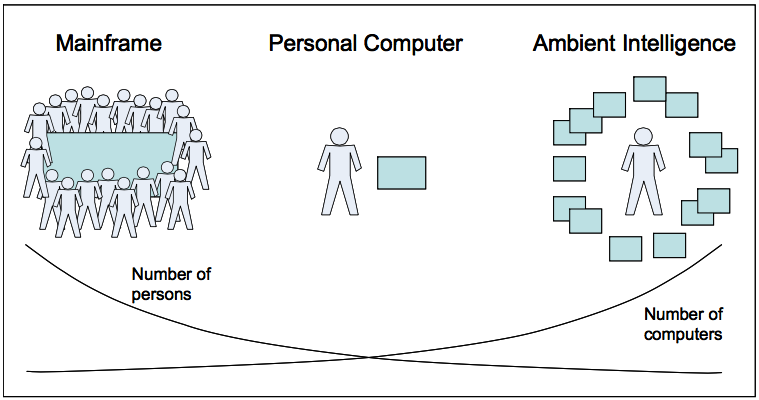
\includegraphics[width=8cm]{figuras/computer_evolution}
        }{
            \Fonte{\citeonline{bick2008ambient}}
        }   
    \end{figure}
    
    
    A computação ubíqua, ou computação pervasiva, apesar de ser fundamentalmente ligada à inteligência ambiental, possui uma diferença conceitual. A computação pervasiva enfatiza a presença de dispositivos físicos distribuídos pelo ambiente e a disponibilidade de recursos sem necessariamente tornar o ambiente inteligente \cite{augusto2007ambient}. A necessidade de uma inteligência comandando os recursos do ambiente é a pedra fundamental do conceito de ambientes inteligentes.
    
    %\subsection{Áreas da Inteligência Ambiental}
    
    Sistemas \acrshort{ami} se relacionam com diversas subáreas da ciência da computação, além da computação ubíqua e inteligência artificial. A grande quantidade de sensores exige uma robusta rede de comunicação. Além disso, a interação entre os dispositivos e as pessoas no ambiente deve ocorrer da forma mais transparente possível, através de interfaces que exijam o mínimo de esforço dos usuários. A inteligência artificial deve permear todas essas áreas, seja otimizando funções do sistema ou provendo mais facilidades ao usuário. A Figura \ref{fig:ami-relation} ilustra as diferentes áreas que fazem parte da inteligência ambiental.
    
    \begin{figure}[h!]
        \centering
        \Caption{\label{fig:ami-relation} Relação entre \textit{AmI} e outras áreas.} 
        \UECEfig{}{
            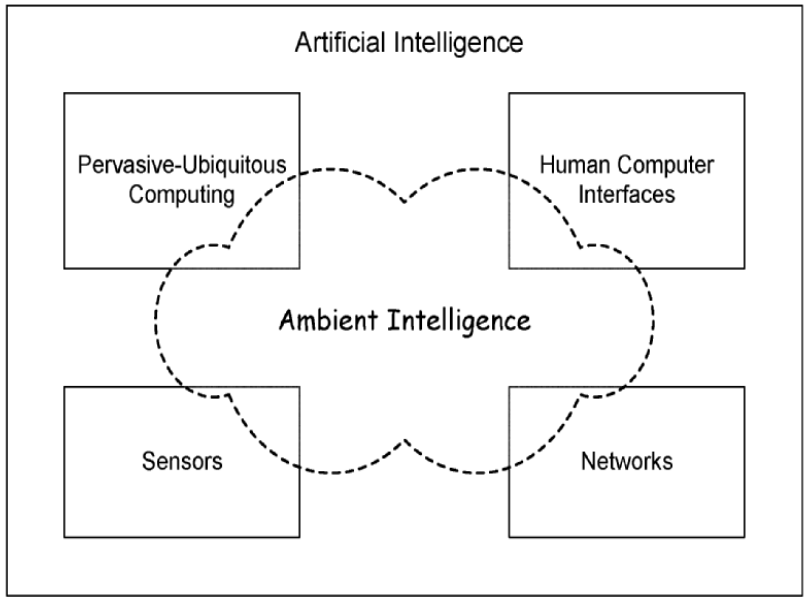
\includegraphics[width=6cm]{figuras/AMI-relations}
        }{
            \Fonte{\citeonline{augusto2007ambient}}
        }   
    \end{figure}
    
    A visão de um futuro cheio de objetos inteligentes e interativos oferece uma gama de oportunidades \cite{bohn2005social}. Ambientes inteligentes podem ser utilizados nos mais diversos contextos. Algumas áreas que podem e até já se beneficiam do uso de sensores e objetos inteligentes são listadas abaixo.
    
    \begin{itemize}
        \item \textbf{Aplicações relacionadas à saúde} -- Objetos inteligentes podem ser utilizados para fornecer serviços de monitoramento e análise dos pacientes de um hospital. Fornecendo aos médicos informações em tempo real do estado de cada um. 
        
        \item \textbf{Serviços de transporte} -- Carros inteligentes já estão em produção, e, apesar de ainda ser uma tecnologia muito nova, já mostra resultados animadores. Eles são equipados com sensores capazes de mapear o ambiente à sua volta e reconhecer outros carros próximos, evitando colisões e melhorando o fluxo de veículos. 
        
        \item \textbf{Serviços de educação} -- Instituições de ensino podem utilizar inteligência ambiental para monitorar seus alunos. Verificando sua frequência em sala de aula, acompanhando o progresso de suas atividades escolares, e, até mesmo, averiguando sua saúde.
        
        \item \textbf{Serviços de emergência} -- Serviços de emergência em geral podem ter um tempo de resposta melhor a um incidente. Por exemplo, casas equipadas com sensores de incêndio poderiam automaticamente enviar a sua localização aos bombeiros quando o fogo fosse detectado.
        
    \end{itemize}
    
    É interessante notar que os dispositivos utilizados em uma aplicação não necessariamente precisam estar no mesmo ambiente. Mais ainda, os objetos de uma aplicação podem ser utilizados não só por um, mas por vários sistemas. Por exemplo, digamos que um paciente esteja sendo monitorado em sua casa através de um conjunto de sensores; esses, por sua vez, enviam todas as informações captadas para o sistema do hospital através da internet. O sistema do hospital processa os dados  e, em caso de emergência, comunica à ambulância mais próxima a localização do paciente, enviando também as informações necessárias para socorrê-lo. Essa conexão entre vários ambientes inteligentes tornou-se possível graças à "\textit{Internet}das Coisas".
  
%\subsection{Internet das Coisas}
%\label{sec:internet-coisas}

    A \textit{Internet das Coisas}, \acrfull{iot}, é um fenômeno tecnológico derivado dos conceitos de comunicação ubíqua e inteligência ambiental \cite{dohr2010internet}. O termo \acrlong{iot} foi usado pela primeira vez no fim da década de noventa, no trabalho de \citeonline{ashton2009internet}, onde uma série de objetos eram capazes de se comunicar através de sensores \acrshort{rfid}, possibilitando uma cooperação entre eles. Com o passar do tempo, esse conceito foi ampliado, permitindo que a comunicação acontecesse por outros meios como a \textit{Internet}, fornecendo, assim, informações e serviços a usuários de diversos locais.
    
    De uma perspectiva mais sistemática, a \textit{Internet das Coisas} pode ser tratada como um sistema altamente dinâmico e radicalmente distribuído, composto por um grande número de objetos inteligentes, produzindo e consumindo informação \cite{miorandi2012internet}.  Esses objetos se comportam como interface entre o mundo real e o virtual. Eles são capazes tanto de sentir fenômenos físicos quanto de produzi-los, traduzindo-os em uma corrente de informações para o mundo virtual e agindo no ambiente físico através de atuadores quando certas condições são alcançadas. 

\section{Programas de Agentes Artificiais Racionais}
\label{sec:agentes}

    Um agente é uma entidade capaz de perceber seu ambiente de tarefa por meio de sensores e agir nele por meio de atuadores. O comportamento de um agente pode ser descrito em termos matemáticos por uma função do agente capaz de mapear qualquer sequência de percepções para uma ação especifica. A função do agente é implementada concretamente pelo programa do agente, que é executado em uma arquitetura adequada (dispositivo de computação com sensores e atuadores físicos). Idealmente, os agentes artificiais racionais, aqui decompostos em um programa de agente e em uma arquitetura, devem agir visando alcançar o melhor resultado esperado, avaliado de acordo com uma medida de desempenho \cite{norvig2004inteligencia}.
    
    \citeonline{norvig2004inteligencia} especificaram quatro tipos básicos de programas de agentes racionais que podem ser adaptadas para resolver problemas em diversos tipos de ambientes de tarefas difíceis. Esses programas incorporam os princípios subjacentes a quase todos os sistemas inteligentes, são classificados levando-se em consideração as informações empregadas no processo de tomada de decisão e as etapas componentes desse processo, ou seja, os agentes reativos simples e sua extensão baseados em modelos empregando regras condição-ação, e os agentes orientados por objetivo e sua extensão orientada por utilidade. Mais recentemente, esboçou-se uma estrutura para o agente com aprendizagem, isto é, a estrutura de um dos quatro tipos básicos com a capacidade de aprendizagem, conseguida pela integração à estrutura básica de três novas etapas à tomada de decisão. A Figura \ref{fig:agente-aprendizado} apresenta o esboço da estrutura do agente com aprendizagem.

    \begin{figure}[h!]
        \centering
        \Caption{\label{fig:agente-aprendizado} Modelo geral de agentes com aprendizado.} 
        \UECEfig{}{
            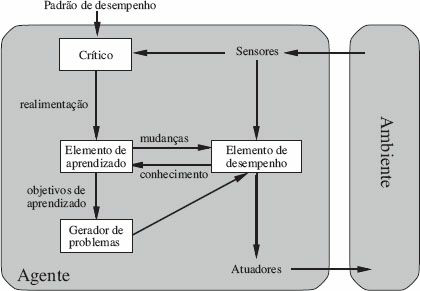
\includegraphics[width=6cm]{figuras/agente-aprendizado}
        }{
            \Fonte{\citeonline{norvig2004inteligencia}}
        }   
    \end{figure}

    \citeonline{wooldridge2009introduction} descreveu formalmente as arquiteturas abstratas do agente reativo e do agente com estado interno, considerando três subsistemas (módulos) de processamento de informação componentes. Em seguida, destacou quatro maneiras diferentes de se concretizar projetos de agentes racionais, ou seja, os agentes lógicos, \textit{subsumption}, \acrshort{bdi}, e com arquiteturas em camadas. A Figura \ref{fig:agente-estado} destaca os três módulos de processamento da informação na arquitetura abstrata do agente com estado interno.
    
    \clearpage
    \begin{figure}[h!]
        \centering
        \Caption{\label{fig:agente-estado} Modelo de um agente com estado interno.} 
        \UECEfig{}{
            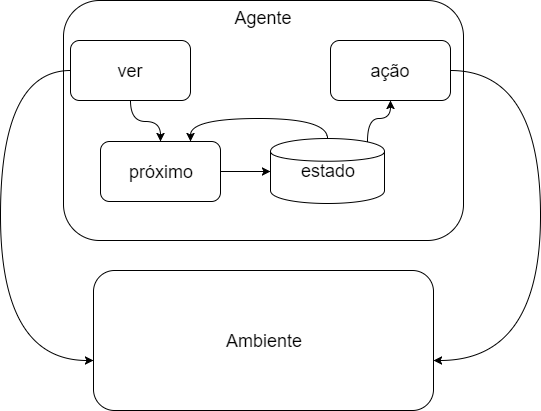
\includegraphics[width=6cm]{figuras/state-agent} %não sei se é a figura correta
        }{
            \Fonte{ Traduzido de \citeonline{wooldridge2009introduction}}
        }   
    \end{figure}
    

    O comportamento do agente com estado interno pode ser resumido da seguinte forma: o agente inicia a partir de algum estado interno \emph{i\textsubscript{0}}, então, observa o estado do seu ambiente \emph{e}, gerando a percepção \emph{ver(e)}. O estado interno do agente é assim atualizado com a função próximo($ver(e), i_0$). O agente então seleciona uma ação com base na função \emph{próximo} da seguinte forma \emph{ação(próximo(ver(e), i\textsubscript{0}))}. A ação é, portanto, executada, e, em seguida, inicia-se um novo ciclo, percebendo o ambiente através da função \emph{ver}, atualizando o estado interno com a função \emph{próximo}, e escolhendo uma ação com a função \emph{ação}. 

    \section{Organizações de Agentes Racionais}
    \label{sec:agent-org}
        
        \acrfull{sma} são conjuntos de agentes que interagem, cooperando para atingir um objetivo comum, ou competindo por recursos no mesmo ambiente. Nesse contexto, uma organização é um padrão de cooperação entre agentes predefinido pelo designer da aplicação, ou gerado pelos próprios agentes a fim de atingir um propósito comum \cite{boissier2004organization}. Em uma casa inteligente, por exemplo, o time de agentes que controla o ambiente deve cooperar para maximizar o conforto das pessoas que residem naquele espaço. 
        
        Mas, para que a organização funcione da melhor forma, é necessário que o projetista seja capaz de resolver dois problemas relacionados ao time de agentes. Primeiro: ele deve ser capaz de criar agentes heterogêneos que, além de agirem de forma individual, sejam capazes de cooperar. Segundo: ele deve criar uma organização racional para esses agentes. Para criar organizações de agentes é necessário descrever formalmente a organização \cite{francoempirical}.
        
    %\subsection{Organização Estrutural}
        \label{subsec:org-struct}
        Organizações representam a racionalização e ordenação de vários instrumentos a fins de se atingir um objetivo específico \cite{selznick1948foundations}. Para que esses objetivos sejam alcançados é necessário subdividi-los em diversos subobjetivos, que contribuem para o propósito geral da organização. Esses subobjetivos são definidos como papéis que são assumidos por agentes dentro de uma organização.
        
        Organizações em \acrshort{sma} são apresentadas normalmente como estruturas monodimensionais. No entanto, na maioria dos casos, são compostas por diversos aspectos estruturais: autoridade, comunicação, delegação, tomada de decisão, poder etc. No trabalho de \citeonline{grossi2005foundations}, as organizações são compostas por três dimensões, chamadas de: \emph{poder}, \emph{coordenação}, e \emph{controle}, onde o \emph{poder} está relacionado à delegação de atividades, a \emph{coordenação} se relaciona ao conhecimento ou compartilhamento de informações, e o \emph{controle} está ligado ao monitoramento de atividades. Formalmente, uma organização é representada pela tupla ilustrada a seguir. 
        
        \begin{equation}
            \centering
            \label{eq:os-structure}
            \langle  R, R_{power}, R_{coord}, R_{control}  \rangle
        \end{equation}
        
        Cada papel em uma organização é assumido por apenas um único agente. Essa imposição torna mais explícita e simples a relação de poder entre os papéis pertencentes à organização. 
        \emph{R} representa o conjunto de todos os papéis da organização e $R_{power}$,  $R_{coord}$, e $R_{control}$ são os relacionamentos entre papéis que caracterizam as estruturas de poder, coordenação, e controle. Tal que, $\forall{r, s}$ $\in$ \emph{R} temos que:
        \begin{equation}
            \label{eq:role-definition}
            \begin{split}
                 (r, s)  \in R_{poder} &\Rightarrow \exists \; R_{coord}(r, s);\\
                 (r, s)  \in R_{poder} &\Rightarrow \exists \;  t \in R \; | \; R_{control}(t, s)
            \end{split}
        \end{equation}
        
        A primeira parte da equação \ref{eq:role-definition} determina que, para toda relação de poder entre o papel \emph{r} e o papel \emph{s}, existe uma relação de coordenação de \emph{r} para \emph{s}. Isso implica que sempre deve haver um fluxo de informação relevante do agente que assume papel \emph{r} para o agente responsável pelo papel \emph{s}. Já na segunda parte da equação, para cada relacionamento de poder entre dois papéis, existe um papel \emph{t} responsável por controlar e monitorar suas ações. A Figura \ref{fig:os-graph} ilustra em um grafo os relacionamentos de uma estrutura organizacional, onde duas subestruturas, A e B, comunicam-se. 
        
        \clearpage
        \begin{figure}[h!]
            \centering
            \Caption{\label{fig:os-graph} Exemplo de uma estrutura organizacional.} 
            \UECEfig{}{
                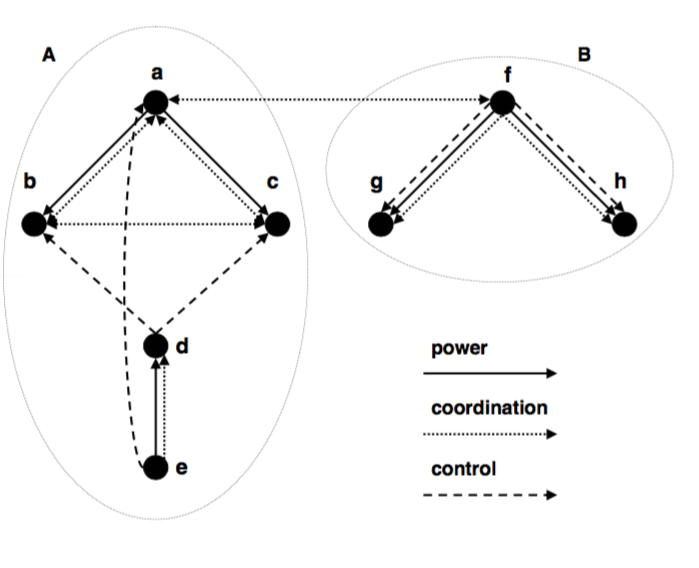
\includegraphics[width=6cm]{figuras/os-graph}
            }{
                \Fonte{ \citeonline{grossi2007structural}}
            }   
        \end{figure}
  
    % INSTITUIÇÕES ELETRONICAS FOI MOVIDO PARA TRABALHOS RELACIONADOS
            
  \section{Engenharia de Sistemas}
        
    O Conselho internacional de Sistemas e Engenharia (\acrshort{incose}) define engenharia de sistemas como uma abordagem interdisciplinar que permite a criação de sistemas. Ela se preocupa em: (1) definir as necessidades do usuário e seus requerimentos no início do ciclo de desenvolvimento; (2) documentar requerimentos; (3) proceder com a síntese de criação; e (4) validar o sistema considerando o problema como um todo. Para a engenharia de sistemas, a chave para a criação de sistemas bem-sucedidos, que satisfaçam os requisitos do cliente dentro de um espaço de tempo esperado, está na definição dos limites do sistema \cite{barry2009agent}.
    
    
    A engenharia de sistemas engloba todas as atividades envolvidas na aquisição, especificação, projeto, implementação, validação, implantação, operação e manutenção dos sistemas sociotécnicos \cite{sommerville2003engenharia}. Os engenheiros de sistemas se preocupam não apenas com o \textit{software}, mas também com o \textit{hardware} e com as interações entre o sistema, os usuários e o ambiente. Eles devem pensar sobre os serviços que o sistema oferece, as restrições sob as quais o sistema deve ser construído e operado e as maneiras pelas quais o sistema é usado para cumprir seu propósito ou finalidade.
    
    O modelo V, ilustrado na Figura \ref{fig:systems-vee}, representa um dos vários ciclos de vida da engenharia de sistemas. Na primeira parte, o modelo descreve detalhadamente o design dos subcomponentes do sistema, até o momento onde se atinge um entendimento mais completo do sistema e de como esses componentes trabalharão. Aí, os componentes são implementados e, em seguida, integrados e testados, até o ponto onde todo sistema esteja completo.
    
    \clearpage
    \begin{figure}[h!]
        \centering
        \Caption{\label{fig:systems-vee}Modelo V de desenvolvimento de sistemas.} 
        \UECEfig{}{
            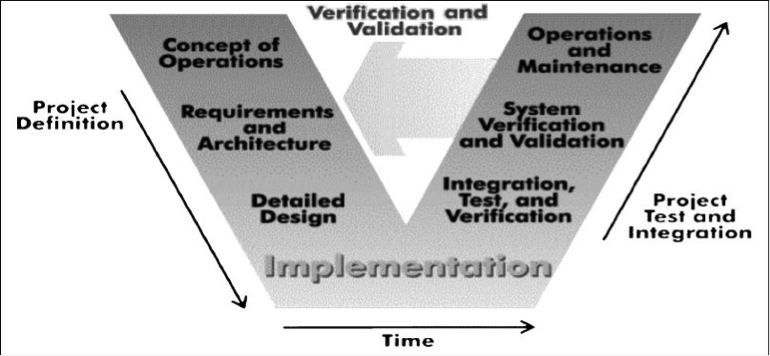
\includegraphics[width=8cm]{figuras/systems-vee}
        }{
            \Fonte{ \citeonline{barry2009agent}}
        }   
    \end{figure}
    
    O processo de desenvolvimento ilustrado na figura \ref{fig:systems-vee} é utilizado na Engenharia de Sistemas devido ao grande número de componentes sendo construídos simultaneamente. Para sistemas que incluem \textit{hardware} ou outros tipos de equipamentos físicos, alterações durante o desenvolvimento dos projetos acabam se tornando muito caras ou mesmo impossíveis. Isso torna necessário que os requisitos do sistema sejam assimilados pelo engenheiro antes de iniciar o desenvolvimento, ou construção, do \textit{hardware}. Porém, a medida que o sistema é instalado, podem ser identificadas limitações no projeto, sejam por problemas no \textit{hardware} ou por requisitos inalcançáveis. 

    Para evitar tal situação, é necessário criar algum projeto inicial para estruturar e organizar o processo de engenharia de requisitos. Nesse projeto, definiremos uma arquitetura de sistemas para, a partir dela, encontrar problemas com os requisitos existentes ou adicionar novos requisitos. Essa abordagem permite que o processo de definição de requisitos e de arquitetura seja tratado como algo contínuo na Engenharia de Sistemas. Consequentemente, podemos pensar nesses processos ligados em uma espiral, como mostra a Figura \ref{fig:espiral-requisitos}.
    
    \begin{figure}[h!]
        \centering
        \Caption{\label{fig:espiral-requisitos} Espiral de requisitos do projeto.} 
        \UECEfig{}{
            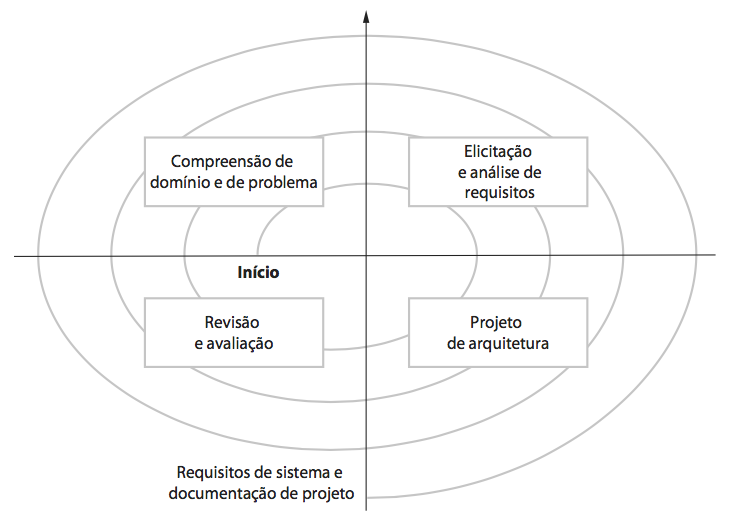
\includegraphics[width=8cm]{figuras/espiral-requisitos.png}
        }{
            \Fonte{ \citeonline{sommerville2003engenharia}}
        }   
    \end{figure}
     
    A espiral mostra como as decisões relacionadas a requisitos podem impactar no projeto e vice-versa. A partir de um ponto inicial, que representa a primeira versão do projeto, a espiral se afasta do centro, passando por todos os quadrantes do plano. Cada volta realizada representa uma nova adição ao projeto, ou um novo requisito.  
    
    De acordo com o Departamento de Defesa dos Estados Unidos \cite{dod2001systems}, a engenharia de sistemas é um processo de gestão interdisciplinar, que busca comprovar, integrar e evoluir um conjunto de soluções, balanceadas através de um ciclo de vida, que ofereçam saídas capazes de satisfazer o cliente. A gestão na engenharia de sistemas visa controlar e integrar os processos que estão sendo construídos. 
    
    %\subsection{Gestão da Engenharia de Sistemas}
        
    A gestão na engenharia de sistemas é alcançada através da integração de três outras atividades, a saber: fase de desenvolvimento; processo de engenharia de sistemas; e ciclo de vida e integração. Cada uma dessas atividades é essencial para atingir uma gestão adequada do desenvolvimento do sistema.
    
    A fase de desenvolvimento é responsável pela conexão entre o design do sistema e a criação, ou aquisição, de tecnologia. Esse processo de desenvolvimento pode ocorrer nos seguintes estágios: (a) em um nível conceitual, onde é produzido um conceito do sistema; (b) em nível de sistema, produzindo uma descrição sobre a performance dele em relação aos seus requisitos; e (c) em nível de subsistema/componente, gerando descrições dos subsistemas/componentes, indicando suas performances e, ainda, uma descrição detalhada das suas características.
    
    O processo de engenharia de sistemas é a etapa mais importante da engenharia de sistemas. O seu propósito é fornecer uma estrutura robusta e flexível, capaz de atender aos requisitos do sistema. Esse processo permite maior controle no desenvolvimento de soluções capazes de atender às necessidades do cliente. Esse procedimento é aplicado em cada nível de desenvolvimento do sistema para produzir uma descrição básica de configuração. Ele segue uma abordagem \textit{top-down}, resolvendo problemas de forma iterativa e recursiva, aplicada de forma sequencial em todos os estágios de desenvolvimento. Esse processo é utilizado para transformar requisitos em um conjunto de produtos do sistema e descrições do processo, adicionando mais detalhes ao desenvolvimento e mais valor, gerando mais informações para auxiliar na tomada de decisões.

    O ciclo de vida e integração se refere às ações associadas ao próprio ciclo de vida do sistema. Ele é necessário para garantir que a solução elaborada pelo sistema seja válida durante toda a sua execução. Essa etapa também inclui o planejamento associado ao desenvolvimento, assim como a integração das múltiplas funcionalidades relacionadas ao \textit{design} e ao processo de engenharia.

%\subsection{Processo de Engenharia de Sistemas}
%\label{subsec:proc-eng-sis}

    No processo de engenharia de sistemas, novas arquiteturas são criadas para descrever e compreender melhor o sistema. A palavra "arquitetura" é utilizada em diversos contextos dentro da engenharia de sistemas, geralmente para descrever como os subsistemas devem ser conectados. No entanto, segundo o \citeonline{dod2001systems}, existem três tipos de arquitetura que podem ser usadas para retratar as diversas características de um sistema, a saber: arquitetura funcional, arquitetura física, e arquitetura do sistema. 
    
    A arquitetura funcional identifica e estrutura os requisitos funcionais e não funcionais. A arquitetura física retrata o sistema final, quebrando-o em diversos subsistemas. A arquitetura de sistemas identifica todos os artefatos relevantes para construir o sistema, incluindo os processos necessários para apoia-lo.
    
    A Figura \ref{fig:sys-eng-process} mostra todas as etapas iniciais do processo de engenharia de sistemas. As atividades fundamentais são a análise de requisitos, análise e alocação funcional, e síntese de \textit{design}, todas coordenadas pelo sistema de análise e controle.
        
    \begin{figure}[h!]
        \centering
        \Caption{\label{fig:sys-eng-process} Processo de Engenharia de Sistemas.} 
        \UECEfig{}{
            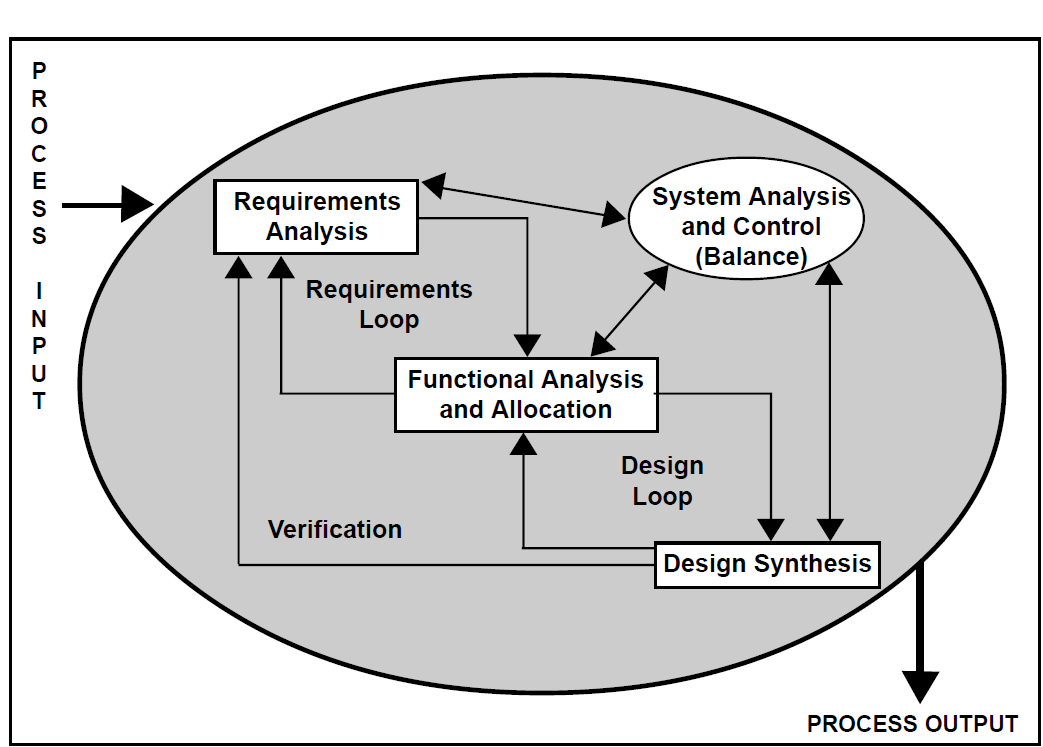
\includegraphics[width=7cm]{figuras/sys-eng-process}
        }{
            \Fonte{ \citeonline{dod2001systems}}
        }
    \end{figure}
    
    A primeira etapa do processo é analisar as entradas. A análise de requisitos é utilizada para desenvolver os requisitos funcionais e não funcionais. Ou seja, as exigências do cliente são traduzidas em um conjunto de requisitos que definem o que o sistema deve fazer e como deve ser seu desempenho. O engenheiro de sistemas deve assegurar que os requisitos sejam compreensíveis, inequívocos, abrangentes, completos e concisos.
    
    Com a análise de requisitos são identificadas funções de alto nível, que são decompostas em diversas funções de baixo nível durante a análise de função. Os requisitos de performance associados a funções de alto nível são alocados para funções de baixo nível. O resultado desse procedimento é uma descrição lógica do sistema em termos de performance. Isso também é conhecido como arquitetura funcional do sistema. A análise funcional e alocação possibilita um melhor entendimento daquilo que o sistema deve fazer, e de como fazer. Além de prover informações sobre as prioridades e conflitos associados às funções de baixo nível, fornecendo informações essenciais para a otimização de problemas físicos.
    
    O \textit{loop} de requisitos compara as funções analisadas e suas performances com seus respectivos requisitos, a fim de aproximar os resultados obtidos com aqueles definidos pelos requisitos. Esse é um processo interativo que revisa os requisitos à medida que sua análise é realizada. 
    
    A síntese de \textit{design} define o sistema em relação aos seus elementos de \textit{hardware} e \textit{software}. Esse processo também é chamado de "arquitetura física". Cada um dos componentes é responsável por, pelo menos, um requisito funcional, e qualquer parte pode ter diversas funções. A arquitetura física é a estrutura básica para definir os parâmetros de especificação do sistema.

    Com o fim da etapa de síntese, os resultados obtidos são comparados com os requerimentos da etapa de análise. Esse processo é chamado de "\textit{loop} de verificação". Cada requisito deve ser examinado. Como esse processo do sistema passa por diversas etapas de desenvolvimento, são necessários diversos métodos de verificação, sendo alguns deles: o exame, a demonstração, a análise (modelagem e simulação), e o teste.
    
    Os sistemas de análise e controle são compostos por técnicas de gestão de atividades necessárias para medir o progresso, avaliar e selecionar alternativas e tomar decisões. Essas atividades são aplicadas em todos os passos do processo de engenharia de sistemas.

\section{Descrevendo Sistemas em Níveis}
\label{sec:abord-def-nivel}

    Segundo \citeonline{wilensky1999thinking}, um sistema pode ser visto como uma unidade funcional devidamente concebida para realizar algum objetivo em algum ambiente. Especificando um pouco mais a ideia, esse tipo de sistema também pode ser visto como um conjunto de partes (componentes) interdependentes que trabalham juntas como uma só, visando realizar o objetivo original do sistema.% A Figura \ref{fig:nivel-1} exemplifica um sistema \acrshort{ami} composto por dois subsistemas. Um representando as pessoas e outro representando o sistema técnico, composto pelo \textit{hardware} e software do sistema.%, com capacidade para satisfazer um objetivo próximo do objetivo original do sistema.
    
    %\begin{figure}[h!]
    %    \centering
    %    \Caption{\label{fig:nivel-1} Visão superficial de um sistema \acrshort{ami}} 
    %    \UECEfig{}{
    %        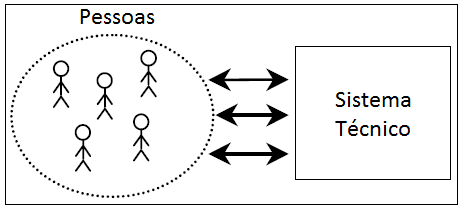
\includegraphics[width=6cm]{figuras/nivel-1}
    %    }{
    %        \Fonte{\cite{davidsson2000multi}}
    %    }   
    %\end{figure}
    
    A noção de níveis de descrição de sistemas historicamente vem sendo utilizada como meio para analisar e compreender uma ampla gama de sistemas naturais. Essa noção pode ser empregada para descrever e compreender melhor diversos tipos de sistemas, desde sistemas que estão em funcionamento atualmente quanto sistemas futuristas, que ainda não estão em funcionamento e são difíceis de projetar.
    
    A noção de nível que está sendo proposta é denominada "visão emergente" de níveis. Essa ideia é bastante diferente da noção de nível em sistemas vistos como hierarquias clássicas, onde o controle do sistema é identificado por meio de uma cadeia de comandos que flui de níveis mais altos para níveis mais baixos, como ilustra a Figura \ref{fig:hierarquia-classica}, em algumas organizações empresariais: o executivo-chefe está no nível superior, depois o presidente, em seguida o vice-presidente, e assim por diante.

    \begin{figure}[!ht]
        \centering
        \Caption{\label{fig:hierarquia-classica} Noção de níveis em uma hierarquia clássica.} 
        \UECEfig{}{
            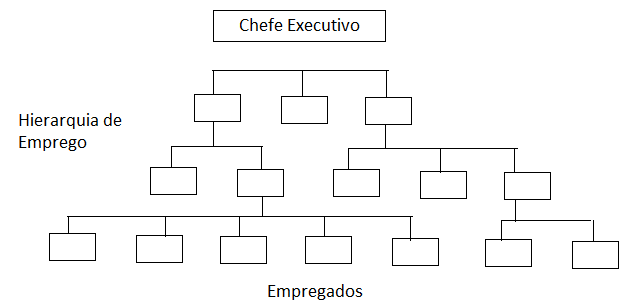
\includegraphics[width=8cm]{figuras/hierarquia-classica}
        }{
            \Fonte{Elaborado pelo autor}
        }   
    \end{figure}
    
    A noção de níveis emergentes, em vez de enxergar CEOs -- gerentes e trabalhadores de linha de montagem dentro de uma hierarquia --, enxerga e descreve uma organização empresarial em termos de divisões corporativas e dos funcionários dentro deles. Por exemplo, a Figura \ref{fig:box-system} ilustra de maneira genérica a descrição em níveis destacando um sistema composto de subsistemas inter-relacionados. Cada um desses subsistemas (A1-A3, B1-B2, C1-C3) pode ser descrito de maneira semelhante até que se atinja um determinado nível inferior de subsistemas elementares.
    
    \begin{figure}[h!]
        \centering
        \Caption{\label{fig:box-system} Diferentes níveis de um sistema simples.} 
        \UECEfig{}{
            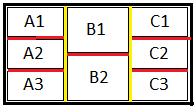
\includegraphics[width=6cm]{figuras/box-system}
        }{
            \Fonte{ Adaptado de \citeonline{simon1996sciences}}
        }   
    \end{figure}
     
    A noção de níveis emergentes é também diferente da noção de nível em sistemas vistos como contêineres, baseada na ideia de partes e todos. Por exemplo, um dia é parte de uma semana, logo, está em um nível mais baixo do que o nível de uma semana, que está em um nível mais baixo do que o nível de um mês, e assim por diante. A visão contêiner difere da visão hierárquica, em que os elementos de um nível inferior são partes dos elementos de um nível superior: um mês é parte de um ano, mas um vice-presidente não faz parte de um executivo-chefe. 
    
    A noção de níveis de descrição, conhecida como "visão emergente" de níveis, foca em fenômenos que surgem de interações de objetos em níveis inferiores. Por exemplo, em sistemas rodoviários urbanos, o engarrafamento que emerge das interações entre os carros nas ruas \cite{wilensky1999thinking}. Menos aparente que o engarrafamento, desempenho de uma divisão corporativa é resultado da complexa rede de relacionamentos e interações entre todos os seus funcionários.   
    Um dos pontos fundamentais quando se pensa em níveis emergentes está no entendimento da noção de comportamento emergente. %nesse caso seria o comportamento emergente inves do objeto???
    O comportamento emergente, ou objeto emergente, depende da forma com a qual o projetista se refere ao sistema. Enxergando o sistema como uma sociedade de (centenas, milhares, \ldots de) objetos separados que cooperam entre si, ou como um único objeto que, sob determinadas condições, pode se dividir em várias partes. Ou seja, o surgimento desse comportamento está relacionado à forma como o projetista enxerga o sistema: referindo-se a ele como como uma unidade, ou como o resultado da interação de diversos componentes, empregando o pronome "ele" ou "eles", ou o verbo "é" ou "são" \cite{wilensky1999thinking}.
    

    Objetos que são vistos como singulares em um nível podem ser melhor compreendidos como plural em outro nível. A capacidade de enxergar o mesmo objeto como singular ou plural, dependendo da situação, permitirá ao projetista de um sistema \acrshort{ami} construir uma compreensão científica mais profunda dos fenômenos intrínsecos ao sistema em desenvolvimento, o que pode ser uma informação valiosa para tomada de decisão na etapa de desenvolvimento
    
    Em sistemas naturais, por exemplo, muitas vezes o objeto emergente observado é descrito de maneira espacial. Isto é, uma aglomeração espacial de componentes (por exemplo, de células), que possui um padrão detectável na sua posição x-y. O padrão emergente não é detectável nas posições x-y, mas por outros parâmetros dos componentes do sistema. Como, por exemplo, a distribuição de velocidades/energias e os desempenhos associados aos componentes, como resultado de uma rede complexa de relacionamentos e interações entre todos os componentes. A Figura \ref{fig:gas-exemplo} ilustra esta ideia para o caso do comportamento de um gás em um recipiente selado. 
    
    \begin{figure}[h!]
        \centering
        \Caption{\label{fig:gas-exemplo} Padrão de comportamento das partículas de um gás.} 
        \UECEfig{}{
            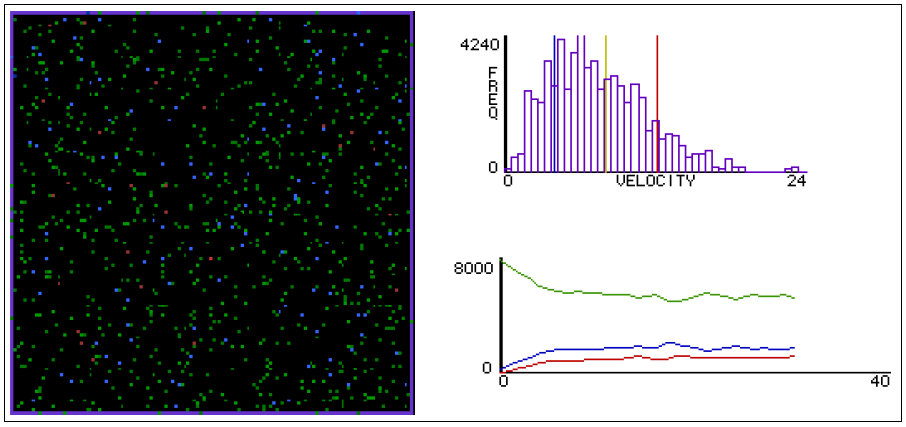
\includegraphics[width=8cm]{figuras/gas-exemplo}
        }{
            \Fonte{\citeonline{wilensky1999thinking}}
        }   
    \end{figure}
    
    
    No exemplo acima, centenas de partículas se encontram em um recipiente fechado. Elas se comportam como bolas de bilhar, colidindo de forma elástica quando se encontram ou quando se chocam com as paredes do recipiente. Todas as moléculas de gás do experimento iniciam em uma mesma velocidade (coloridas em verde). À medida que colidem podem acelerar (se colorindo de vermelho) ou desacelerar (coloridas em azul). Esse experimento foi realizado com intuito de ilustrar a distribuição de Maxwell-Boltzmann. Após um número de interações, a quantidade de partículas azuis (lentas) aumenta e a velocidade das partículas vermelhas cresce, de forma que a energia do gás como um todo permanece constante. Essa reação continua até o momento em que as velocidades se estabilizam, formando as distribuições ilustradas na Figura \ref{fig:gas-exemplo}.

    Assim como no caso dos sistemas naturais, parâmetros associados a componentes que são observados ao longo do tempo são um padrão mais difícil de detectar, resultando em um objeto emergente que é menos perceptível e menos óbvio. No entanto, uma distribuição de velocidades em um sistema \acrshort{ami} e uma aglomeração espacial, como as partículas de um gás, de componentes em um sistema natural, estão na mesma categoria, ou seja, fundamentalmente ambos podem ser vistos como objetos emergentes.
  
\begin{comment}


\section{Moise}
\label{sec:moise}

    A linguagem de modelagem organizacional Moise \cite{hubner2002model, hubner2007developing} descreve formalmente uma organização de agentes. Essa organização pode ser descrita através da especificação organizacional, \acrfull{os}, que pode ser dividida em três dimensões, \acrfull{ss}, \acrfull{fs}, \acrfull{ds}. A especificação estrutural (\acrshort{ss}) determina os papéis e seus relacionamentos, além dos grupos que compõem a organização. A especificação funcional (\acrshort{fs}) define os objetivos globais e o modo como eles serão alcançados. E por fim, a especificação deôntica (\acrshort{ds}) relaciona essas duas dimensões, identificando qual conjunto de objetivos e funções da camada funcional será atribuído a cada papel da camada estrutural. 

    %VERIFICAR NOMES DOS RELACIONAMENTOS STRUCTURAL SPECIFICATION
    Mais precisamente, a especificação estrutural é construída em três níveis, individual, social, e coletivo. No nível individual a \acrshort{ss} determina qual papel cada agente deverá assumir e quando. O nível social determina o relacionamento entre os papéis, sendo que os três tipos de relacionamento são: $authority$, $comunication$, e $acquaintance$. Onde um relacionamento $authority$ entre papéis implica na existência de uma ligação de $comunication$, que por sua vez implica numa relação de $acquaintance$ entre os papéis. E no nível coletivo a especificação estrutural define em quais grupos os papéis serão agregados.
    
    Essas descrições do \acrshort{ss} indicam um subconjunto de papéis que devem ser representados no grupo e sua cardinalidade miníma e máxima, representando a quantidade de agentes que podem assumir o mesmo papel simultaneamente. Além de definir subgrupos e relacionamentos com outros grupos. A Figura \ref{fig:moise-franco}(a) ilustra uma \acrshort{ss} do \emph{Moise} onde um grupo de agentes \emph{Gr} pode assumir dois papéis distintos, \emph{C} e \emph{S}, e um outro grupo de agentes pode assumir o papel \emph{L}. 
    
    \begin{figure}[h!]
        \centering
        \Caption{\label{fig:moise-franco}Estrutura organizacional de um time de agentes.} 
        \UECEfig{}{
            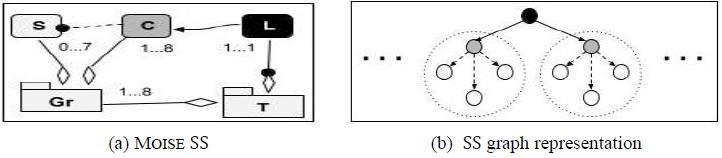
\includegraphics[width=10cm]{figuras/moise-franco}
        }{
            \Fonte{ \cite{francoempirical}}
        }   
    \end{figure}
    
    A partir da especificação estrutural do Moise podemos estabelecer uma relação entre os papéis de agentes na forma de um grafo, onde os papéis de agente são os vértices e os relacionamentos entre os papéis ($authority$, $comunication$, e $acquaintance$) são as arestas. o grafo da Figura \ref{fig:moise-franco}(b) representa a estrutura organizacional do time gerada a partir da \acrshort{ss} da Figura \ref{fig:moise-franco}(a).
    
\section{Instituições Eletrônicas}
\label{sec:fund-org-ei}
    %%%organizar e escrever o que for necessario!!!!!
    O comportamento de um sistema é definido pela forma como seus elementos relacionam, seja para atingir um determinado objetivo ou competir por um conjunto de recursos. Para definir formalmente esse comportamento, precisamos de um protocolo capaz de descrever todos os tipos de mensagens que os componentes de um \acrshort{sma} enviem entre-si. Para descrever  esse processo utilizamos uma versão mais sofisticada de uma máquina de estado não determinística, também conhecida como \acrfull{ei} \cite{rodriguez1999towards}.
    
    Essa semelhança com máquinas de estado finito confere a \acrshort{ei} diversas vantagens para a formalização de protocolos de interação. Existem diversas técnicas que automatizam o processo de verificação de propriedades de um determinado estado. Por exemplo, não devem existir estados que um agente jamais deve alcançar, ou estados onde uma vez alcançados não exista mais saída. Essas propriedades podem ser observadas com algoritmos básicos de teoria dos grafos.
    
    Neste trabalho utilizaremos uma versão simplificada da \acrshort{ei} utilizada no trabalho de \citeonline{vasconcelos2002approach}. Nessa versão simplificada a \acrshort{ei} é formada por um conjunto de \emph{cenas} conectadas através de \emph{transições}. Assumindo que exista uma linguagem de comunicação \emph{CL} entre os agentes e instituição eletrônica, uma \emph{cena} pode ser definida da seguinte forma:
    
    Para ilustrar melhor essa definição, a Figura \ref{fig:agora-exemplo} ilustra um exemplo de uma cena para \emph{agora room} \cite{miller1988markets}. Neste exemplo temos um agente comprador interagindo com uma série de agentes vendedores. Essa cena foi simplificada removendo negociações e leilões. O comprador anuncia os produtos que tem interesse, verifica as ofertas dos vendedores e escolhe a mais barata. 
    
    \begin{figure}[h!]
        \centering
        \Caption{\label{fig:agora-exemplo} Exemplo de cena} 
        \UECEfig{}{
        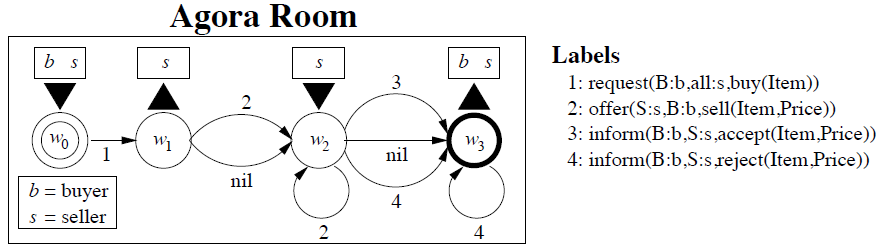
\includegraphics[width=12cm]{figuras/agora-exemplo}
        }{
        \Fonte{\cite{vasconcelos2002approach}}
        }   
    \end{figure}
    
    Na cena temos dois papéis, \emph{b} e \emph{s} representando respectivamente comprador e vendedor. O estado inicial $w_0$ é representado pelo par de círculos concêntricos, e estado final $w_3$ é simbolizado pela circulo mais denso. Os estados de acesso são marcados pelas caixas contendo os papéis e setas apontados para baixo, e os estados de saída são marcados pelas setas apontando para os papéis. Agora que definimos uma cena podemos definir uma \acrlong{ei}.
    
    \begin{theorem}
        Uma \acrshort{ei} é uma tupla $\varepsilon = \langle SC, T, S_0, S_\Omega, E, \lambda_E \rangle$ onde:
        \begin{itemize}
            \item SC = \{$s_1, \ldots, s_n$\} é um conjunto de finito não vazio de cenas;
            \item T  = \{$t_1, \ldots, t_m$\} é um conjunto finito e não vazio de transições;
            \item $s_0 \in SC$ é a cena raiz;
            \item $S_\Omega \in SC$ é a cena de saída;
            \item $E = E^I \cup E^O$ é um conjunto de arcos tal que $E^I \subseteq WE^S \times T$ é um conjunto de arestas dos estados de saída $WE^S$ da cena S, e $E^O \subseteq T \times WA^S$ é o conjunto de arestas de entrada dos estados $WA^S$ da cena S;
            
            \item $\lambda_E : E \mapsto p(x_1, \ldots, x_k)$ mapeia cada transição para um predicado correspondendo a suas restrições.
        \end{itemize}
    \end{theorem}
    
    As transições são conexões entre cenas pelas quais os agentes se movem, possivelmente trocando papéis e sincronizando seus movimentos com outros agentes. A Figura \ref{fig:ei-example} ilustra a definição acima através de um exemplo mais complexo do \emph{agora market} \cite{miller1988markets}. Essa \acrshort{ei} exige que os agentes passem por uma etapa de admissão antes de entrarem para o mercado, depois que a \emph{agora room} é finalizada compradores e vendedores quitam suas dívidas. 
    
    \begin{figure}[h!]
        \centering
        \Caption{\label{fig:ei-example} Exemplo de instituição eletrônica} 
        \UECEfig{}{
        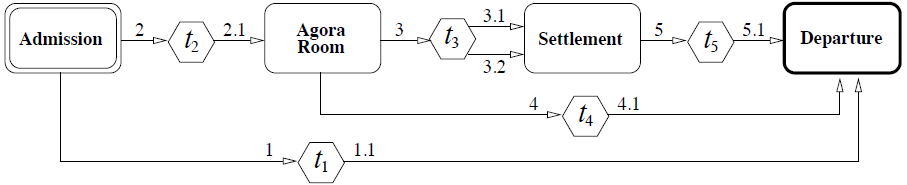
\includegraphics[width=12cm]{figuras/ei-example}
        }{
        \Fonte{\cite{vasconcelos2002approach}}
        }   
    \end{figure}
    
    Cada cena da instituição eletrônica é representada pelos retângulos de bordas arredondadas, onde o retângulo duplo representa a cena inicial, e o retângulo com bordas mais grossas caracteriza a cena final. Cada transição é simbolizada por hexágonos, e as linhas que ligam transições à cenas são os estados de saída ou acesso. 
    

\end{comment}
	\chapter{Trabalhos Relacionados}
\label{cap:trabalhos-relacionados}


\citeonline{parunak1998agent} comparam duas formas de modelagem para a simulação de um sistema de cadeia de suprimentos. A primeira utiliza uma série de fórmulas matemáticas para simular o comportamento do sistema com o passar do tempo. A segunda utiliza  modelagem baseada em agentes para construir virtualmente o sistema e observar seu funcionamento. Como conclusão, o autor define que, para sistemas centralizados, é mais apropriado o uso de modelagens com base matemática. Dessa forma, a modelagem baseada em agentes deve ser usada em sistemas com alto grau de distribuição.

\citeonline{norling2000enhancing} utiliza modelagens baseadas em agentes para construir simulações da sociedade humana capazes de exibir comportamentos mais realistas. Para alcançar esse resultado, os agentes que compõem a simulação utilizam um mecanismo de tomada de decisão chamado \textit{NDM (Naturalistic Decision Making)}, que leva em consideração diversos fatores além da racionalidade para tomar uma decisão. 

\citeonline{davidsson2000multi} realiza um estudo sobre o uso de modelagens centralizadas e descentralizadas no processo de criação de simulações. Para ilustrar o estudo são demonstrados  os processos para uma simulação de sistema de desenvolvimento de \textit{software}, tanto de forma centralizada quanto descentralizada, comparando cada uma das metodologias e gerando um conjunto de diretrizes que auxiliam o uso de simulações baseadas em agentes.
 
\citeonline{davidsson2005distributed} utilizam \acrshort{mabs} para modelar e simular um sistema que monitora e controla um escritório em um prédio comercial. O grande diferencial da abordagem proposta nesse trabalho é que todos os componentes do sistema (as pessoas, o \textit{hardware}, e o próprio \textit{software} do sistema)  são representados na modelagem por agentes inteligentes. Utilizando essa abordagem, eles definem diversos comportamentos para cada um dos agentes, apresentando o desempenho do sistema com essa variação.

\citeonline{mustafa2013simulation} descreve o processo de desenvolvimento de um simulador para aplicações em \acrfull{aal}. Assim como aplicações \acrshort{ami}, sistemas de vivência assistida geram grandes fluxos de informação e dependem de sensores espalhados em um determinado ambiente. A aplicação descrita no trabalho utiliza um conjunto de regras sobre uma base de dados para gerar um sistema de inferência. Essas regras são determinadas por especialistas, mas o sistema é capaz de armazenar os dados coletados pelos sensores e utilizá-los para adaptar a aplicação às necessidades de cada usuário. 

\citeonline{macal2014introductory} apresentam um conjunto de boas práticas relacionadas ao desenvolvimento de sistemas, utilizando modelagem baseada em agentes. Eles descrevem os contextos onde essa técnica pode ser utilizada, os tipos de agentes modelados e os tipos de relacionamentos elaborados a partir deles.

\citeonline{francoempirical} tratam de um problema de organização e \textit{design} de times de agentes em um ambiente de competição onde cada um dos times deve disputar os recursos disponíveis em um ambiente. Apesar da abordagem do trabalho ser diferente, o problema é bastante similar ao enfrentado na elaboração de projetos de sistemas \acrshort{ami}, onde, dependendo da aplicação, podemos ter diversas entidades com objetivos conflitantes (\textit{software} vs \textit{hardware}, ou \textit{software} vs usuário).

\citeonline{grossi2005foundations, grossi2007structural} estabelecem um conjunto de técnicas que auxiliam na avaliação de organizações multiagentes. Em seus trabalhos são definidos diversos conceitos, baseados na teoria dos grafos, para extrair características como robustez, flexibilidade e eficiência de uma determinada organização. Essas características são utilizadas para comparar diferentes organizações quanto ao seu desempenho para a resolução de um determinado problema.

\citeonline{barry2009agent} defendem que a utilização de simulações dirigidas por agentes (\acrshort{ads}) é essencial para a construção de sistemas complexos. A aplicação de \acrshort{ads} em conjunto com técnicas de engenharia de sistemas pode prover uma maior compreensão do sistema como um todo, facilitando seu \textit{design} e melhorando sua performance. 

Dentre as vantagens da utilização de \acrshort{ads} no processo de desenvolvimento, \citeonline{barry2009agent} destacam as seguintes: (1) pode ser usada como uma ferramenta de geração de requerimentos; (2) permite prototipar e analisar funções do sistema; (3) pode ser usada como plataforma de visualização; (4) um componente pode ser usado para representar vários outros, modificando certas características para dar mais realismo à simulação; (5) o experimento pode ser realizado nos mais diversos contextos, ilustrando desde cenários ideais até ambientes catastróficos para o sistema. 

\citeonline{hubner2002model, hubner2007developing} descrevem a linguagem de modelagem organizacional Moise, que representa formalmente uma organização de agentes. Essa organização pode ser descrita através da especificação organizacional, \acrfull{os}, que pode ser dividida em três dimensões: \acrfull{ss}, \acrfull{fs}, \acrfull{ds}. A especificação estrutural (\acrshort{ss}) determina os papéis e seus relacionamentos, além dos grupos que compõem a organização. A especificação funcional (\acrshort{fs}) define os objetivos globais e o modo como eles serão alcançados. E, por fim, a especificação deôntica (\acrshort{ds}) relaciona essas duas dimensões, identificando qual conjunto de objetivos e funções da camada funcional será atribuído a cada papel da camada estrutural. 

%%%intituições Eletronicas

\citeonline{rodriguez1999towards} definem,  em seu trabalho sobre \acrfull{ei}, um protocolo capaz de representar sistemas complexos através de máquinas de estado. Em uma Instituição Eletrônica, cada estado simboliza uma cena e cada cena possui um conjunto de estados que representam as entidades que compõem o sistema. A utilização de máquinas de estado permite a automatização do processo de verificação das propriedades de um determinado estado. Cada uma ilustra um aspecto do sistema que será desenvolvido, detalhando as entidades envolvidas e as relações entre elas. 

%\section{Metodologia AVA}
%\label{sec:ava}

\citeonline{garcia2010human} definiram a metodologia AVA, que é um conjunto de procedimentos que guiam o desenvolvedor na definição, criação, teste e validação do sistema \acrshort{ami}.  O foco do seu trabalho é auxiliar na criação de ambientes inteligentes através de um paradigma de simulação onde cada componente é estudado separadamente. A simulação é criada a partir de uma modelagem de sistemas multiagentes, onde cada agente é especificado de acordo com um componente e suas interações.

A partir da definição dos modelos do ambiente e dos usuários são instanciados os modelos do sistema \acrshort{ami} a ser simulado. Com a implementação desses modelos, são executadas diversas simulações e em seguida seus resultados são analisados a fim de detectar \textit{bugs} ou melhorias possíveis no sistema. Cada mudança no sistema reinicia o ciclo da metodologia, refatorando a modelagem da aplicação, seus modelos e suas implementações. Esse ciclo deve continuar até o ponto onde o desenvolvedor considera que o sistema é estável. 

Um outro conceito bastante interessante inserido no trabalho de \citeonline{garcia2010human} é a noção de inserção de realidade. Se o desenvolvedor da aplicação não encontrar erros na simulação, ele pode inserir elementos do mundo real na simulação de forma gradual, controlando cada etapa do sistema. A cada novo elemento "injetado", o ciclo de modelagem/simulação é repetido, tornando o sistema cada vez mais robusto. Esse processo pode continuar até o ponto onde todo o sistema tenha sido implantado no mundo real. 

\section{Considerações}

O trabalho de \citeonline{parunak1998agent} é utilizado como base para conceitos empregados não só em seu trabalho mas também em vários dos outros trabalhos citados neste capítulo. A modelagem de sistemas multiagentes (\acrshort{mabs}) é um conceito fundamental dos trabalhos de \citeonline{davidsson2005distributed}, que serviram como a inspiração inicial deste projeto. Nesses trabalhos, \citeonline{davidsson2000multi} utiliza \acrshort{mabs} para modelar e simular não só sistemas mas também seus usuários e os equipamentos que o compõem. O trabalho de \citeonline{norling2000enhancing} também utiliza esse tipo de modelagem para simular pessoas, porém, diferente de \citeonline{davidsson2000multi}, seu objetivo não é o aperfeiçoamento do sistema, mas sim gerar agentes com um comportamento mais humano.

Dentre as linguagens de modelagem para \acrshort{sma}, a linguagem \textit{Moise} \cite{hubner2002model, hubner2007developing} descreve formalmente organizações de agentes através de três modelos que se complementam. No trabalho de \citeonline{rodriguez1999towards}, os \acrshort{sma} são descritos através das instituições eletrônicas, capazes de definir os protocolos de comunicação entre cada entidade. A linguagem Moise, apesar de fornecer uma excelente representação da organização de agentes, não ilustra com naturalidade as interações entre as entidades. Por outro lado, as instituições eletrônicas explicitam os protocolos de comunicação entre os agentes de uma organização, mas podem ser bastante complexas para certos tipos de sistema. 

A metodologia AVA \cite{garcia2010human} define um conjunto de procedimentos que guiam o desenvolvedor na definição, criação, teste e validação de sistemas \acrshort{ami}. Para isso, ela utiliza uma série de simulações baseadas em sistemas multiagente, que, aos poucos, evoluem o sistema até o ponto em que o desenvolvedor considere suficiente para inserir elementos reais. A inserção de componentes reais do sistema na simulação é chamada de inserção de realidade, e permite que, aos poucos,  os componentes da simulação sejam substituídos por elementos do mundo real, até o ponto em que o sistema esteja totalmente implantado no mundo em seu ambiente físico.

Apesar de auxiliar em diversas etapas da construção e simulação de sistemas \acrshort{ami}, a metodologia AVA não define uma abordagem para determinar os comportamentos dos agentes que compõem o sistema ou a simulação. A abordagem nesta dissertação utiliza conceitos propostos em \acrshort{mabs} para definir um processo de simulação de sistemas, focando em sistemas \acrshort{ami}, utilizando como base alguns dos conceitos propostos nos trabalhos de \citeonline{hubner2007developing} e \citeonline{rodriguez1999towards}. definindo um modelo comportamental, estrutural e funcional para os agentes do sistema. 



	\chapter{Definição do Modelo FEC} %Metodologia
\label{cap:abordagem}

    O projeto de sistemas de Inteligência Ambiental complexos (sistemas \acrshort{ami}), compostos por outros sistemas menores, é uma tarefa complexa que exige um alto grau de planejamento. A falha do desenvolvedor em enxergar, de forma correta, o resultado das interações entre os diversos componentes projetados para o sistema pode causar perdas na qualidade do serviço a ser ofertado e, ainda, desperdício de tempo/dinheiro para corrigir erros na etapa de implementação. Essa tarefa fica ainda mais complexa à medida que o sistema cresce em número de componentes e, consequentemente, de interações entre eles, principalmente se a aplicação tiver um caráter inovador e original.

    A engenharia de sistemas define uma série de métodos, ilustrados no diagrama V na Figura \ref{fig:systems-vee}, que podem auxiliar no projeto e no teste dos sistemas \acrshort{ami}. A parte da descida do modelo V, que diz respeito às etapas aconselhadas para o projeto, compreende a definição dos conceitos da aplicação, sendo elas: análise de requisitos, análise funcional e a síntese do projeto. Em seguida, durante a etapa de implementação, a parte da subida do modelo V orienta a definição e execução de diversos tipos de testes, verificação e validação do sistema projetado. 

    A abordagem proposta neste capítulo consiste em uma contribuição à etapa de análise funcional do sistema. Permitindo o estudo de \textit{feedbacks} para refinar as etapas de análise de requisitos e de síntese do projeto. Mais especificamente, a abordagem permitirá ao projetista realizar estudos experimentais, visando verificar/encontrar decomposições funcionais alternativas de subsistemas componentes capazes de atender aos requisitos funcionais e de desempenho do sistema \acrshort{ami}. 
    
    Como resultados, tais estudos poderão indicar ao projetista a necessidade de se revisar a etapa de análise de requisitos para resolver problemas funcionais. Isso pode levar a mudanças na etapa de síntese de projeto e, consequentemente, na busca de uma arquitetura física adequada, em termos de componentes de \textit{hardware} e de \textit{software} componentes do sistema. 
    
    A ideia principal da abordagem está em representar, formalmente, determinadas decomposições funcionais do sistema \acrshort{ami} através de organizações de programas de agentes artificiais. Em seguida, utilizar uma plataforma de simulação multiagente adequada ao formalismo proposto, que permita ao projetista entender melhor o comportamento do sistema \acrshort{ami} em projeto, analisando seu desempenho em diferentes cenários do ambiente de tarefas, prevenindo erros e auxiliando a construção de projetos mais eficientes. A abordagem propõe um quadro formal para o projetista empregar na representação das organizações de programas em seus aspectos funcionais, estruturais e comportamentais.
    
    As duas próximas seções apresentam a abordagem proposta. A Seção \ref{sec:pontos-propostas} define como o projetista deve enxergar o sistema \acrshort{ami} para que ele possa ser representado por uma organização de programas de agentes racionais. A Seção \ref{subsec:desc-fec} descreve o quadro formal, denominado modelo \acrshort{fec}. Finalmente, o Capítulo \ref{cap:resultados} descreve como organizações, formalizadas por meio do modelo \acrshort{fec}, podem ser executadas em uma plataforma de simulação multiagente permitindo a observação do desempenho de um sistema \acrshort{ami} associado à medida que os programas interagem entre si e com um ambiente de tarefas simulado.
    
\section{Principais Pontos de Vista e Propostas na Abordagem}
\label{sec:pontos-propostas}

Esta seção descreve os principais pontos de vista e propostas na abordagem para ajudar no projeto de sistemas \acrshort{ami}. São elas: 

\begin{itemize}
    \item[\textbf{P1} -] Definição de sistema de Inteligência Ambiental (sistema \acrshort{ami}) como um conjunto formado por um sistema técnico que interage com um ambiente de tarefas contendo pessoas, visando realizar algum objetivo original.
    
    \item[\textbf{P2} -] Definição de sistema técnico como um composto de \textit{hardware} e \textit{software}, onde cada um de seus elementos pode ser representado por um agente artificial. Composto de uma arquitetura e um programa de agente.
    
    \item[\textbf{P3} -] Descrição informal de um sistema \acrshort{ami} por meio de uma organização de programas de agentes racionais, para representar tanto o \textit{software} quanto o \textit{hardware} e as pessoas usuárias do sistema técnico. 
    
    \item[\textbf{P4} -] Descrição informal de uma organização com muitos programas de agentes interagindo em pelo menos dois níveis diferentes de aprofundamento/especificação.
    
    \item[\textbf{P5} -] Descrição formal da organização de programas de agentes, representando o sistema \acrshort{ami} em seus aspectos funcionais (modelo $F$), estruturais (modelo $E$) e comportamentais (modelo $C$) – modelo $FEC$ da organização.
    
    \item[\textbf{P6} -] Utilização de estratégias de simulação baseada em agentes e a noção de objetos emergentes, que são medidas (distribuições) associadas ao desempenho do sistema técnico e de cada um de seus subsistemas componentes, previamente formalizados em um modelo \acrshort{fec} de uma organização de programas de agentes, como meio de avaliar o desempenho de um sistema em projeto em um ambiente de tarefas virtual.
    
    \item[\textbf{P7} -] Execução de simulações que permitam ao projetista entender como os efeitos da aleatoriedade das ações (falhas), de alguns componentes do sistema interferem na forma e nas propriedades macro de uma distribuição.
    
    \item[\textbf{P8} -] Simulação das condições de atuação do sistema técnico e das pessoas no ambiente real do sistema \acrshort{ami}. Simulação do comportamento dessas pessoas em programas de agentes na organização representando pessoas.
    
    \item[\textbf{P9} -] Definição da noção de caso de teste para avaliar o desempenho de um sistema \acrshort{ami} em projeto, como sendo qualquer configuração particular do ambiente de tarefas simulado. Ainda, um conjunto de casos de teste descreve diferentes configurações ambientais, isto é, problemas de diferentes níveis de dificuldade para o sistema, que permitem ao projetista entender e dominar os mecanismos que causam a emergência de diversas distribuições associadas aos componentes do sistema técnico.
    
\end{itemize}

    Mais explicitamente, a proposta \textbf{P1} considera que um sistema de Inteligência Ambiental (sistema \acrshort{ami}) é composto por um sistema técnico e pelo sistema ambiental. O sistema técnico trata de todo o conjunto \textit{hardware}/\textit{software}, tais como: sensores, atuadores, artefatos computacionais, serviços e aplicações de software. Em aplicações \acrshort{ami}, o sistema técnico deve, de maneira não intrusiva, perceber informações de seu ambiente de tarefa, e, a partir delas, selecionar ações a serem executadas.    
    
    O sistema ambiental é composto por tudo que foge do controle do projetista na aplicação, ou seja, as pessoas e o próprio ambiente. Dessa forma, o sistema técnico interage com o ambiente e com as pessoas que circulam por ele, buscando realizar algum objetivo original (função global do sistema). A Figura \ref{fig:sistema-tec-p1} ilustra a ideia de um sistema \acrshort{ami} visto como um composto integrado de pessoas e um sistema técnico composto por duas partes principais. 

   
    \begin{figure}[h!]
        \centering
        \Caption{\label{fig:sistema-tec-p1} Separação do sistema \acrshort{ami} em sistema técnico e ambiental.} 
        \UECEfig{}{
            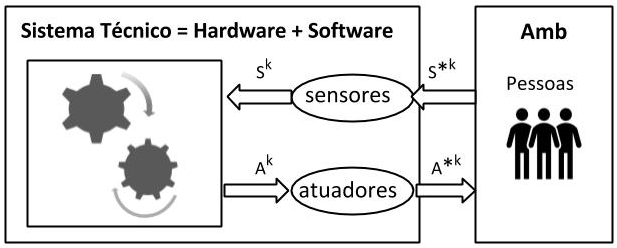
\includegraphics[width=8cm]{figuras/sistema-tec-p1}
        }{
            \Fonte{Elaborada pelo autor.}
        }   
    \end{figure}
    
    Muitos sistemas técnicos atuais são distribuídos e envolvem uma interação complexa entre pessoas e máquinas. Por exemplo, pode-se imaginar o \textit{hardware} em um ambiente semelhante a um prédio, incluindo os sensores e atuadores, e o \textit{software} para monitorar e controlar o \textit{hardware} no prédio, visando satisfazer as pessoas, por exemplo, adaptando a temperatura e a intensidade da luz de acordo com as preferências destas pessoas, e gastando o mínimo de energia possível, por exemplo, desligando automaticamente as lâmpadas e o ar-condicionado de salas vazias.
    
    A proposta \textbf{P2}, em resumo, considera que o sistema técnico da aplicação \acrshort{ami} pode ser representado por um ou mais agentes artificiais. Isto é, um sistema formado por uma arquitetura, ou seja, algum tipo de dispositivo computacional com sensores e atuadores físicos, e por um programa de agente que implementa a função do agente, e mapeia percepções em ações. A arquitetura disponibiliza ao programa as percepções de seus sensores. O programa é executado para selecionar as ações de acordo com as informações recebidas. E, por fim, as ações são executadas pelos atuadores definidos na arquitetura. Cada programa de agente pode incorporar uma série de componentes funcionais associados à (\emph{subsistemas}) percepção (\emph{ver}), atualização de estado interno (\emph{próximo}) e tomada de decisão (\emph{ação}).
    
    Assim, de acordo com a abordagem, qualquer sistema técnico poderá ser abstraído pela noção de agente artificial. Podem ser sistemas simples, como um ar-condicionado com controle inteligente, um robô mais sofisticado para prestar serviços de interesse das pessoas, ou mesmo um sistema técnico complexo, composto de vários subsistemas (agentes artificiais) conectados por um modelo de cooperação/competição, onde cada subsistema pode usar funcionalidades de outros para compensar ou complementar a sua própria funcionalidade, visando realizar o objetivo original do sistema \acrshort{ami}.
    
    Com relação às duas primeiras propostas: a proposta \textbf{P3} considera que o sistema \acrshort{ami} pode ser descrito informalmente como uma organização de programas de agentes capazes de representar tanto o \textit{software} ($AgSoftware$) quanto o comportamento de grande parte do \textit{hardware} ($AgHardware$) que compõe a arquitetura do sistema técnico, e, ainda, das pessoas usuárias ($AgPessoas$) deste sistema. A Figura \ref{fig:org-agentes-p3} ilustra tal ideia, considerando a ideia de sistema \acrshort{ami} na Figura \ref{fig:sistema-tec-p1}.
    
    \begin{figure}[h!]
        \centering
        \Caption{\label{fig:org-agentes-p3} Representação dos componentes de um sistema \acrshort{ami} como agentes inteligentes.} 
        \UECEfig{}{
            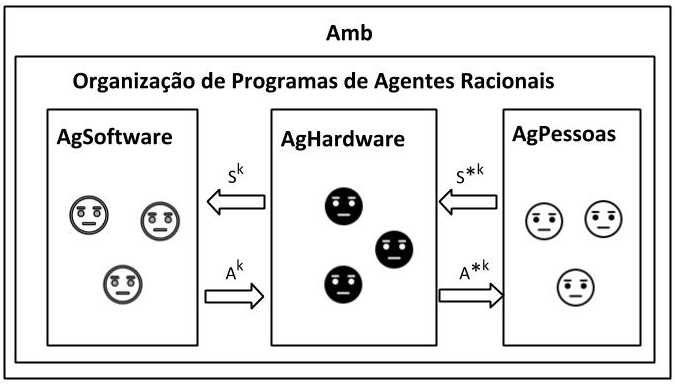
\includegraphics[width=8cm]{figuras/org-agentes-p3.png}
        }{
            \Fonte{Elaborado pelo autor.}
        }   
    \end{figure}
    
    Ou seja, além de definir o software do sistema ($AgSoftware$) como programas de agentes, que seriam responsáveis por monitorar e controlar o hardware do sistema. A abordagem propõe modelar tanto o comportamento dos usuários, quanto o desempenho dos sensores e atuadores definidos na arquitetura do sistema. Utilizando programas de agentes racionais, respectivamente denominados $AgPessoas$ e $AgHardware$. À medida do possível, considerando esta generalização, a descrição informal deve indicar o esboço de uma estrutura e do comportamento desejado para o grupo de programas na organização. Eles devem ser adequados ao ambiente de tarefas e, consequentemente, ao alcance do objetivo original do sistema.
    
    Em \textbf{P4}, a proposta é que uma organização com muitos programas de agentes interagindo, seja descrita informalmente em pelo menos dois níveis diferentes de aprofundamento/especificação. O objetivo é analisar e compreender melhor o sistema AmI, dessa forma: 
    
    \begin{itemize}
        
        \item Nível 1: a aplicação \acrshort{ami} abstraída é como uma única entidade, formado por um sistema técnico (agente artificial). Descrito por uma organização de programas de agentes composta por um único programa do tipo $AgSoftware$ . Que interage com pelo menos um programa de agente do tipo $AgHardware$, para representar sensores e atuadores capazes de interagir com um ambiente, que pode conter programas de agentes do tipo $AgPessoas$ (Figura \ref{fig:org-level-p4}a); 
        
        \item Nível 2:  a aplicação \acrshort{ami} é abstraída como uma entidade composta por vários sistemas técnicos (agentes artificiais) conectados. O sistema \acrshort{ami} é descrito por uma organização de organizações de programas de agentes, cada uma descrevendo um dos sistemas técnicos componentes (Figura \ref{fig:org-level-p4}b). 
    
    \end{itemize}
    
    \begin{figure}[h!]
        \centering
        \Caption{\label{fig:org-level-p4} Diferentes níveis de abstração de um sistema \acrshort{ami}.} 
        \UECEfig{}{
            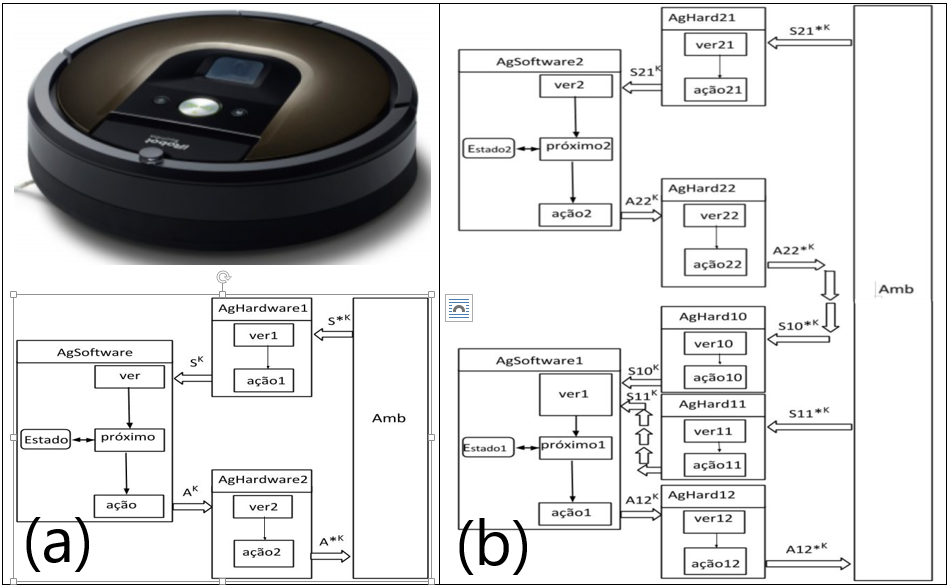
\includegraphics[width=10cm]{figuras/org-level-p4.png}
        }{
            \Fonte{Elaborado pelo autor.}
        }   
    \end{figure}
    
    Tomemos como exemplo uma aplicação de inteligencia ambiental, em que o sistema é responsável por manter o ambiente limpo, enquanto pessoas transitam pelo ambiente. A Figura \ref{fig:org-level-p4}a ilustra a situação onde esse sistema \acrshort{ami} é modelado por um único sistema técnico, ou seja, um robô aspirador de pó. Descrito por uma organização composta por um programa de agente $AgSoftware$, capaz de controlar o aspirador de pó, e dois programas de agente $AgHardware1$ e $AgHardware2$, para representar respectivamente um sensor e um atuador do sistema técnico no ambiente. No exemplo, enquanto que o programa $AgSoftware$ é do tipo com estado interno, os programas $AgHardware1$ e $AgHardware2$ são do tipo reativo simples.
    
    Já a Figura \ref{fig:org-level-p4}b ilustra a situação desse mesmo sistema \acrshort{ami}. Porém, modelado por dois sistemas técnicos. Agora além do sistema técnico que representa os aspiradores de pó, temos um outro sistema para monitorar ambiente. Este utilizaria um conjunto de câmeras estáticas para reconstruir o estado do ambiente, incluindo a posição do robô aspirador de pó. O primeiro sistema técnico, o aspirador, descrito pela organização formada pelos programas $AgSoftware1$, $AgHard10$, $AgHard11$ e $AgHard12$, utiliza a funcionalidade de localização global gerada pelo segundo sistema técnico, o de monitoramento, descrito pela organização formada pelos programas $AgSoftware2$, $AgHard21$ e $AgHard22$, para selecionar uma estratégia mais inteligente de navegação e limpeza.
    
    A proposta em \textbf{P5} é que a organização de programas de agentes, representando o sistema \acrshort{ami}, seja especificada previamente em seus aspectos funcionais (modelo F), estruturais (modelo E) e comportamentais (modelo C), empregando um formalismo adequado. O modelo F proposto refere-se à descrição formal da função global (objetivo original) de uma parte da organização de programas representando o sistema técnico; o modelo E refere-se à descrição formal da estrutura visível da organização de programas representando o sistema \acrshort{ami}; e o modelo C refere-se à descrição formal dos processos que ocorrem dentro desta organização e, principalmente, como os programas de agentes representando o sistema técnico devem se comportar para alcançar os resultados desejados no ambiente de tarefas.
    
    Em seguida à proposta, \textbf{P6} recomenda utilizar simulação baseada em agentes, e a noção de objetos emergentes, como meio de avaliar o desempenho de um sistema em projeto, previamente formalizado em um modelo \acrshort{fec} de uma organização de programas de agentes. Mais especificamente, a abordagem propõe que as interações entre os programas na organização, e desta com o ambiente de tarefas, seja simulada durante um período de tempo. Assim o desenvolvedor pode perceber se a estrutura, descrita no modelo $E$, e o comportamento integrado destas entidades, descrito no modelo $C$, funcionam de maneira a realizar o objetivo original do sistema, descrito no modelo $F$.
    
    Mais especificamente, a abordagem propõe que a execução de simulações de modelos \acrshort{fec} em ambientes de tarefas virtuais, em diferentes configurações e devidamente programados em linguagem adequada. A partir das simulações são extraídos objetos emergentes, que são medidas (distribuições) associadas ao desempenho do sistema técnico e de cada um de seus subsistemas componentes. Observando esses objetos emergentes, o desenvolvedor tem uma melhor noção da capacidade do sistema de cumprir seu objetivo original. A Figura \ref{fig:sim-emergente-p6} ilustra esta ideia.
        
    \begin{figure}[h!]
        \centering
        \Caption{\label{fig:sim-emergente-p6} Fluxo de extração dos objetos emergentes.} 
        \UECEfig{}{
            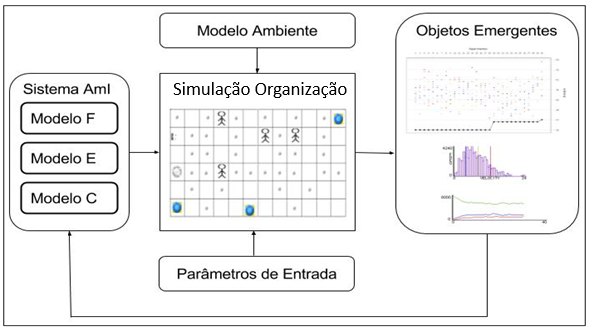
\includegraphics[width=10cm]{figuras/sim-emergente-p6.png}
        }{
            \Fonte{Elaborado pelo autor.}
        }   
    \end{figure}
    
    Assim, uma distribuição associada a um parâmetro de algum dos programas de agentes, componentes do sistema técnico, pode ser vista como uma descrição do que emerge das interações do sistema com seu ambiente de tarefas. Isso permite ao projetista avaliar as propriedades macro das distribuições associadas ao programa de agente como, por exemplo: média, variância e desvio padrão. Como consequência, o desenvolvedor poderá dominar os mecanismos que causam a emergência destes objetos e utilizar a seu favor na economia de esforço e tempo para o desenvolvimento de um sistema \acrshort{ami} racional. 
    
    Neste contexto, a proposta \textbf{P7} coloca em destaque particular o caso de ambientes de tarefas não determinísticos. A abordagem considera que o projetista deve buscar entender como os efeitos da aleatoriedade das ações de alguns componentes do sistema técnico interferem na forma e nas propriedades macro de uma distribuição. Este entendimento deve servir para garantir que os componentes de confiabilidade baixa, integrados e implementados em um sistema \acrshort{ami} realizarão o objetivo desejado em seu ambiente de tarefas.
    
    A proposta \textbf{P8} pode ser dividida em duas. Primeiro, a abordagem propõe que os programas de agentes $AgPessoas$ devem simular o comportamento dos usuários do sistema. Essa imitação deve ser suficiente para que o efeito de suas ações no ambiente simulado gere como resposta, um comportamento correspondente adequado dos programas de agentes dos tipos $AgHardware$ e $AgSoftware$ representando o sistema técnico. Segundo, propõe também que o ambiente de tarefas virtual deve simular adequadamente as condições de atuação do sistema técnico e das pessoas no ambiente real. 
    
    Sabe-se que a natureza de qualquer ambiente de tarefa pode ser classificada de acordo com sete dimensões (propriedades), sendo elas: observável-parcialmente observável, determinístico-estocástico, episódico-sequencial, estático-dinâmico, discreto-contínuo, agente único- multiagente, e conhecido-desconhecido. Assim, a abordagem considera que, em conjunto com outros objetos presentes em um ambiente real, estas propriedades devem ser também adequadamente simuladas. 
    
    Finalmente, a proposta \textbf{P9}, considera que uma configuração particular do ambiente simulado define um caso de teste para o sistema \acrshort{ami} em projeto, e que diferentes configurações compreendem a diferentes casos de teste. Definindo problemas de diferentes níveis de dificuldade para o sistema. Por exemplo, considerando-se um sistema \acrshort{ami} composto por um sistema técnico formado por uma certa quantidade de robôs para atuar em um local semelhante a um aeroporto, uma configuração particular do ambiente deve definir o número de obstáculos, de lixo e de pessoas em locais específicos do aeroporto. Neste tipo de ambiente, algumas configurações podem exigir dos robôs maior consumo de energia, enquanto que outras podem colocar lixo em locais de mais fácil acesso aos robôs.
    
\begin{section}{Modelo FEC de uma Organização de Programas}
\label{subsec:desc-fec}

    Conforme dito na introdução da seção anterior, para avaliar o alcance de um objetivo original por parte de um sistema \acrshort{ami} em projeto, o projetista deve considerar a relação existente entre três partes. Sendo elas: (1) o objetivo original do sistema, (2) o seu ambiente interno, aqui representado por uma organização de programas de agentes, e (3) o ambiente de tarefas em que o sistema funciona. De acordo com a proposta, para concluir que o sistema \acrshort{ami} é adequado ao ambiente de tarefas, o projetista necessita comprovar primeiro que organização de programas alcança o objetivo original do sistema. Então ele poderá concluir que o projeto do ambiente interno do sistema está caminhando na direção da adequação ao ambiente externo. 

    \citeonline{norvig2004inteligencia} enfatizam a importância de se especificar adequadamente a natureza dos ambientes de tarefas, durante o projeto de sistemas compostos por agentes artificiais. Dependendo da natureza destes ambientes, o projetista pode entender a sua tarefa em diferentes graus de complexidade. Variando desde problemas bem definidos, em ambientes de tarefas observáveis, determinísticos e estáticos. Até problemas difíceis de exploração, em ambientes de tarefas parcialmente observáveis, não determinísticos, dinâmicos, desconhecidos e multiagentes competitivos. A literatura sobre o assunto disponibiliza diversas referências. Elas apresentam diversos resultados de abordagens para sistemas de agentes artificiais em todos estes ambientes de tarefas.

    O modelo \acrshort{fec} aqui proposto visa permitir que o projetista formalize adequadamente o primeiro e segundo termos dessa relação. Permitindo uma descrição matemática e computacional deles. Dessa forma facilitando que as organizações de programas de agentes, associadas aos sistemas \acrshort{ami} em projeto, possam ser implementadas, simuladas e avaliadas quanto a realização do seu objetivo original. No que diz respeito à formalização da organização (2), o modelo \acrshort{fec} visa permitir que o projetista se concentre nas partes (estruturas) de uma organização, no entendimento de como estas partes funcionam (comportamentos) e o que fazem (funções). Neste contexto, a simulação de um modelo \acrshort{fec} permitirá ao projetista perceber relações, que podem não ser aparentes, entre as estruturas possíveis, os comportamentos e as funções de uma organização representando um sistema \acrshort{ami}.
    
    \subsection{Modelo de Função (F)}
    \label{modelo-fec-f}
    
    O modelo de Função ($F$) de uma organização refere-se à descrição formal da função global (objetivo original) do sistema \acrshort{ami} (ou de algum de seus subsistemas). Este modelo deve estar em sintonia com algumas das saídas da etapa de análise de requisitos, no processo de engenharia do sistema. Mais especificamente, o modelo $F$ permite que o projetista formalize os objetivos dos atores interessados e envolvidos com o processo. Além de orientar o projetista com mais clareza na especificação do modelo estrutural (E) e do modelo comportamental ($C$) da organização de programas de agentes. Esta formalização permite que o projetista obtenha uma medida de satisfação do objetivo do sistema \acrshort{ami}. Determinando o desempenho da organização interagindo com um ambiente de tarefas virtual. É a partir da especificação do modelo $F$ da organização que o projetista deve definir os objetos emergentes (medidas e distribuições) das simulações de interações da organização com o ambiente virtual, visando avaliar o desempenho dos componentes do sistema, especificados previamente na etapa de análise funcional.

    A proposta considera que alguns dos objetivos originais dos atores interessados no projeto, descrevem determinadas exigências em relação ao sistema \acrshort{ami} pretendido. Outros objetivos podem descrever funções relevantes do sistema, ou qualidades que o sistema pretendido deve alcançar ou fornecer. Voltando ao exemplo do aspirador de pó. Pode ser requisitado ao sistema, que além de manter um determinado local  (ambiente) limpo, ele deve também minimizar o uso dos recursos disponíveis. Utilizando, por exemplo, um software de monitoramento e controle para otimizar a movimentação dos robôs.
    
    Os objetivos originais articulam as necessidades percebidas, desejos e requisitos a alcançar com as decisões relacionadas ao projeto do sistema AmI. Estes objetivos podem expressar generalidades (p.ex., melhorar a qualidade dos serviços) e, frequentemente, não podem ser diretamente quantificados, necessitando maiores esclarecimentos em termos de objetivos próximos que sejam mensuráveis. Assim, o projetista deve definir formalmente estes objetivos próximos como substitutos do objetivo original, e seus valores de importância no contexto do objetivo original, indicando como os objetivos próximos contribuem com diferentes graus para a satisfação do objetivo original.
    
    Por exemplo, no caso do sistema \acrshort{ami} para limpeza de ambientes públicos mencionado. O projetista pode definir que o objetivo original ($O_0$) do sistema técnico consiste em prestar um serviço de alta qualidade, com um mínimo de despesas e o máximo de educação com as pessoas presentes no ambiente. Como consequência, de maneira a satisfazer o objetivo original sistema, o projetista pode definir para os agentes aspiradores pelo menos quatro objetivos próximos possíveis de serem medidos, ou seja: manter o ambiente limpo ($O_1$), manter energia suficiente na bateria ($O_2$), trabalhar em equipe ($O_3$) e cumprimentar as pessoas ($O_4$).
    
    De acordo com o esquema de decomposição do objetivo original proposto. A ideia no modelo $F$ é que o projetista deve definir, formalmente, o objetivo original do sistema \acrshort{ami} por meio de uma função de utilidade que considera: (1) um vetor de funções escalares associadas aos objetivos próximos; e (2) os valores de importância destes objetivos no contexto do objetivo original. Cada função escalar ($av_i$) no modelo $F$ associa valores no domínio dos números reais com um conjunto de episódios possíveis ($Ep$), descritos em termos de um conjunto de estados do ambiente (percepções $S$) e um conjunto de ações possíveis para o sistema ($A$).
    
    Por exemplo, a Tabela \ref{tab:asp-resultados} exemplifica alguns valores de satisfação/insatisfação nos objetivos próximos $O_1$ e $O_2$ (funções escalares $av_1$ e $av_2$), relacionados aos objetos emergentes de energia e limpeza, medidos em diversos episódios ($Ep_k$) na história das interações (k) mantidas por um programa de agente aspirador de pó em um ambiente de tarefas simulado. Os valores das funções indicam que cada agente artificial deve se movimentar e limpar um ambiente, maximizando os níveis de limpeza do ambiente e de energia em sua bateria ao final da tarefa.
    
    \begin{table}[h!]   
        \centering
        \Caption{\label{tab:asp-resultados} Histórico de ações do agente aspirador}
        \UECEtab{}{
            \begin{tabular}{ccclll}
                \toprule
                    $Ep^K $ & $S^K$ & $A^K$ & $av_1(Ep^K)$ & $av_2(Ep^K)$ \\
                \midrule \midrule
                  k  & \ldots L \ldots & asp & \phantom{-}0.0  & -1.0 \\
                  k+1  & \ldots L \ldots & les, oes, nor, sul  & \phantom{-}1.0  & -2.0 \\
                  k+2 & \ldots L \ldots & nop & \phantom{-}0.0  & \phantom{-}0.0 \\
                  k+3  & \ldots S \ldots & asp & \phantom{-}2.0  & \phantom{-}1.0 \\
                  k+4  & \ldots S \ldots & les, oes, nor, sul  & -1.0  & -2.0 \\
                  k+5  & \ldots S \ldots & nop & -1.0  & \phantom{-}0.0\\
                \bottomrule
            \end{tabular}
        }{
        \Fonte{Elaborado pelo autor}
    }
    \end{table}
        
    A segunda coluna ($S^k$) descreve uma parte das informações nas percepções do agente em cada episódio possível ($L$ = local limpo; $S$ = local sujo). A terceira coluna ($A_k$) descreve as ações possíveis para o agente nestes episódios ($asp$ = aspirar; $les$ = leste; $dir$ = direita; $oes$ = oeste; $nor$ = norte; $sul$ = sul; $nop$ = não operar). Na quarta e quinta colunas ($av_1$ e $av_2$), respectivamente associadas aos objetivos de limpeza ($O_1$) e de energia ($O_2$), as funções escalares para medir a satisfação destes objetivos pelo agente em cada episódio de sua história no ambiente de tarefas. 
    
    O restante desta seção formaliza as funções de avaliação e a função utilidade, componente principal do modelo F, que podem ser utilizadas para medir o desempenho de sistemas \acrshort{ami} do interesse do projetista. Ou seja, o modelo F permite que a performance de cada um dos agentes componentes do sistema e, mais especificamente, dos programas de agentes dos tipos $AgSoftware$ e $AgHardware$, componentes do sistema técnico, seja mensurada. Esses componentes podem ser identificados como $AgentAmI$ no quadro  formal abaixo. O quadro apresenta o esquema de representação e a definição correspondente dos principais termos envolvidos na definição da função utilidade:
    
    \begin{itemize}
        
        \item S = {$s_1$, $s_2$, \ldots} -- estados do ambiente do agente – em qualquer instante k o ambiente está em um dos estados do conjunto de estados do ambiente;
        
        \item A = {$a_1$, $a_2$, \ldots} -- capacidade efetuadora do agente – um conjunto de ações possíveis de serem executadas pelos atuadores do agente em qualquer instante k;
        
        \item ação : $S^*  \rightarrow A$ -- comportamento de um agente -- uma função que mapeia sequências de estados do ambiente $s \in S^*$ em ações $a \in A$, ou seja, intuitivamente, um agente decide que ação executar baseado em sua história, sua experiência até o momento da decisão;
        
        \item amb : $S\times A  \rightarrow S$ -- comportamento (determinístico) de um ambiente – uma função que mapeia o estado corrente do ambiente $s \in S$ e uma ação $a \in A$, em um estado $amb(s,a)$ resultantes da execução da ação $a$ no estado $s$;
        
        \item AgentAmI -- um programa de agente implementando concretamente a função ação de um dos agentes nos conjuntos de agentes $AgPessoas$, $AgHardware$ e $AgSoftware$;
        
        \item Amb -- um programa ambiente implementando a função amb, capaz de interagir com um programa AgentAmI por meio de algum protocolo de interação;
        
        \item $\Omega$ -- um conjunto de descrições de cenários de ambientes de tarefa factíveis de instanciar em Amb e avaliar AgentAmI;
        
        \item $Cenario_i \in \Omega$ -- uma descrição específica de cenário ambiental;
        
        \item $Cenarios \in P(\Omega$) -- um subconjunto de descrições de cenários ambientais (conjunto de casos de teste);
        
        \item $h(Cenario_i) \in (S\times A)N^{Int}$ -- história de comprimento $Nint$ de $AgentAmI$ em $Amb$ correspondente ao $Cenario_i \in \Omega$ – uma sequência $s_0 \xrightarrow{a_0} s_1 \xrightarrow{a_1} s_2 \xrightarrow{a_2} \ldots s_{Nint-1} \xrightarrow{a_{Nint-1}} s_(Nint)$, tal que $s_0$ é o estado inicial do ambiente, $a_{Nint-1}$ é a última ação que o agente escolheu para executar, e $s_{Nint}$ é o último estado do ambiente;
        
        \item $Ep^k(h(Cenario_i)) \in (S\times A)$ -- episódio na interação k, $k \leq Nint$, da história de $AgentAmI$ em $Amb$ correspondente ao caso $Cenario_i \in \Omega$;
    
        \item $H(Cenarios) \in P((S\times A)N^{Int})$ -- conjunto de histórias de comprimento $NInt$ de $AgentAmI$ em $Amb$ considerando $ProtocolInteracao$ e todos os cenários ambientais em $Cenarios \in P(\Omega)$;
    \end{itemize}
    
    Considerando o esquema de representação acima. O objetivo original a ser alcançado por um programa $AgentAmI$, em um ambiente de tarefas simulado por um programa $Amb$, pode ser formalizado por meio de um vetor de $M (M \geq 1)$ funções objetivo próximo (implícitas) do objetivo original estabelecido pelo projetista. Considerando um conjunto de cenários em H(Cenários), temos:

    \begin{equation}\label{eq:func-cen}
        f(H(Cenarios)) = f_1(H(Cenario), f_2(H(Cenario), \ldots, f_M(H(Cenario) \in R^M
    \end{equation}
        
    Supondo-se que o número de cenários no conjunto H(Cenários) seja $NCenarios$, a satisfação de um objetivo próximo $m (m = 1 \ldots M)$ alcançado por um $AgentAmI$ em $Amb$ pode ser formalizada:

    \begin{equation}\label{eq:func-cen-media}
        f_m(H(Cenarios)) = \frac{1}{NCenario} \sum_{i=1}^{NCenario} av_m(h(Cenario_i))
    \end{equation}

    Supondo-se que o comprimento de cada história do programa $AgentAmI$ em $Amb$ seja $NInt$, o valor medido de recompensa/penalização em um objetivo próximo m, alcançado pelo programa $AgentAmI$ em $Amb$ considerando o $Cenario_i \in \Omega$, pode ser formalizada: 
        
    \begin{equation}\label{eq:func-av}
        av_m(h(C_i)) = \sum_{k=1}^{Nint} av_m(Ep^k(h(Cenario_i)))
    \end{equation}
    
    tal que $av_m(Ep_k(h(Cenario_i)))$ é o valor medido de recompensa/penalização no objetivo próximo $m$ atribuído ao episódio $k$ da história associada ao $Cenario_i \in \Omega$. 
    
    Finalmente, a função Utilidade permitirá ao projetista obter medidas de desempenho de $AgentAmI$ em $Amb$ considerando um conjunto de cenários ambientais em $H(Cenarios)$. Supondo-se que o grau de utilidade de um objetivo próximo independe dos valores assumidos pelos demais (função é preferencialmente independente), este trabalho considera uma forma especial de função utilidade, ou seja, uma função aditiva no formato linear:
    
    \begin{equation}\label{eq:func-util}
        Utilidade(f(H(Cenarios))) = \sum_{m=1}^M w_m \cdot f_m(H(Cenario)))
    \end{equation}
    tal que $w_m \geq 0$, $m =1, \ldots, M$.
    
    Por exemplo, a Figura \ref{fig:func-objetivo-asp} ilustra os valores da função objetivo próximo de energia ($f_1$) e os valores de função utilidade, considerando também os valores de uma função objetivo próximo de limpeza ($f_2$), ao longo de cem, considerando dez cenários ambientais em cada um. 
    
    \begin{figure}[h!]
        \centering
        \Caption{\label{fig:func-objetivo-asp} Função objetivo em diversos cenários.} 
        \UECEfig{}{
            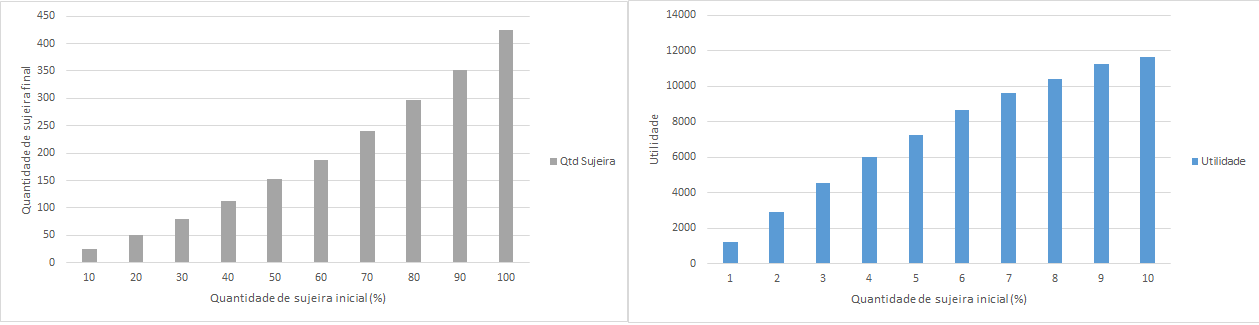
\includegraphics[width=14cm]{figuras/func-objetivo-asp-rob.png}
        }{
            \Fonte{Elaborado pelo autor.}
        }   
    \end{figure}

    Além de ajudar ao projetista a avaliar o desempenho de cada um dos programas de agentes artificiais em uma organização projetada, ou seja, dos subsistemas técnicos componentes do sistema técnico no sistema \acrshort{ami}, as medidas obtidas com estas funções de utilidade em simulações permitirão ao projetista realizar um julgamento a respeito do comportamento da organização de programas de agentes racionais em particular e, consequentemente, do próprio sistema \acrshort{ami} em projeto.
    
    \subsection{Modelo de Estrutura (E)}
    
    O projeto de uma estrutura organizacional de programas de agentes artificiais adequada a um ambiente de tarefas. Capaz de representar satisfatoriamente um sistema \acrshort{ami} em projeto, é um problema combinatório complexo. Ainda mais considerando os muitos subsistemas técnicos, componentes e a quantidade de interações possíveis (conexões) entre eles. O projetista precisa montar e escolher uma estrutura adequada para o sistema. Isto é, definir o número e os tipos de subsistemas, assim como quais subsistemas devem interagir entre si, de maneira que o comportamento resultante dessa integração seja adequado ao seu ambiente de tarefas. Maximizando a função de utilidade que foi definida no modelo F da organização de programas de agentes representando o sistema. 
    
    Mais especificamente, o modelo E de uma organização de programas de agentes refere-se à descrição formal da sua estrutura. O modelo visa contribuir com a busca de soluções para o problema de projeto de estruturas organizacionais que possam ser facilmente testadas em simulações em computador. 
    
    O quadro formal que define o modelo E proposto pode ser dividido em duas partes. A primeira parte permite ao projetista definir o conjunto de programas de agentes, conjunto de papéis que esses programas podem assumir na organização e as relações entre esses papéis,. Além dos grupos de programas e a cardinalidade destes grupos. A segunda parte do modelo permite ao projetista definir o mapa das interações que ocorrem entre os programas de agentes em diferentes papéis dentro dos grupos que compõem a organização. O quadro abaixo apresenta o esquema de representação adotado e a definição correspondente dos principais termos componentes do modelo:
    
    \begin{itemize}
    
        \item Agents -- representa um conjunto de $N_A$ programas $AgentAmI$ na organização (lembrar que, no modelo $F$, $AgentAmI$ foi definido como um programa de agente implementando concretamente a função ação de um dos agentes nos conjuntos de agentes $AgPessoas$, $AgHardware$ e $AgSoftware$);
        
        \item Roles -- representa um conjunto de $N_R$ papéis que podem ser atribuídos aos programas de agentes $AgentAmI \in Agents$;
        
        \item AgentRoles -- uma família de $N_R$ conjuntos do tipo $AgentAmIR_j (j = 1 \ldots N_R)$, onde cada conjunto $AgentAmI_{Rj}$ é formado por $N_{Rj}$ programas $AgentAmI \in Agents$ desempenhando o papel $R_j \in Roles$;
        
        \item Groups -- uma família de NG conjuntos de programas de agentes, onde cada conjunto identifica um grupo de agentes exercendo seus papéis na organização;
        
        \item Bond -- uma família de relações do tipo $Bond_x(AgentAmI_{Ri}, AgentAmI_{Rj})$, onde cada relação $Bond_x(AgentAmI_{Ri}, AgentAmI_{Rj})$ representa uma relação binária de um tipo $x \in \{knowledge, control, coordination, authority\}$, existente entre os programas de agentes no conjunto $AgentAmIR_{i} \in AgentsRoles$ e os programas de agentes no conjunto $AgentAmIR_{j} \in AgentsRoles$, tal que para todo $Agent_1 \in AgentAmIR_{i}$ e todo $Agent_2 \in AgentAmIR_{j}$:
          
            \begin{itemize}
                \item se ($Agent_1, Agent_2) \in Bond_{knowledge}(AgentAmIR_{i}, AgentAmIR_{j})$ então o agente $Agent_1$ (agente no papel $r_i$) tem o conhecimento da existência do agente $Agent_j$ (agente no papel $R_j$);
                
                \item se ($Agent_1, Agent_2) \in Bond_{control}(AgentAmIR_{i}, AgentAmIR_{j})$ então o agente $Agent_1$ deve monitorar as atividades do $Agent_2$, e assumir as tarefas que este não conseguir realizar;
                
                \item se ($Agent_1, Agent_2) \in Bond_{coordination}(AgentAmIR_{i}, AgentAmIR_{j})$ então cada ato de informação do programa $Agent_1$ ao programa $Agent_2$ gera o conhecimento correspondente no programa $Agent_2$;
                
                \item se ($Agent_1, Agent_2) \in Bond_{authority}(AgentAmIR_{i}, AgentAmIR_{j})$ então toda delegação de tarefas do programa $Agent_1$ ao programa $Agent_2$ cria uma obrigação correspondente no programa $Agent_2$;
                
            \end{itemize}
        
        
        \item Communication -- uma relação em $Agents \times Agents$ descrevendo formalmente quem pode enviar mensagens para quem na organização de agentes;
        
        \item Frequency -- uma matriz sociométrica associando a cada par de agentes $(AgentAmI_x, AgentAmI_y) \in  Communication$, um valor linguístico de frequência $f_{xy}$ (p. ex: $f_{xy} = \{baixa, media, alta\}$ indicando a frequência com que, em geral, um agente $AgentAmI_x \in Agents$ troca mensagens com outro agente $AgentAmI_y \in Agents$.

        
    \end{itemize}
    
    Por exemplo, a parte superior da Figura \ref{fig:asp-estrutura} ilustra um sistema \acrshort{ami} envolvendo cinco pessoas usuárias e um sistema técnico composto por três aspiradores de pó. Todos inseridos em um cenário ambiental representando um ambiente físico (prédio), dividido em três áreas distintas. A parte inferior esboça uma estrutura para uma organização formada por onze programas de agentes correspondentes, representando tanto as pessoas usuárias quanto os componentes do sistema técnico do sistema \acrshort{ami} nas três áreas.
    
    \begin{figure}[h!]
        \centering
        \Caption{\label{fig:asp-estrutura} Ambiente de tarefas e organização de programas de agentes.} 
        \UECEfig{}{
            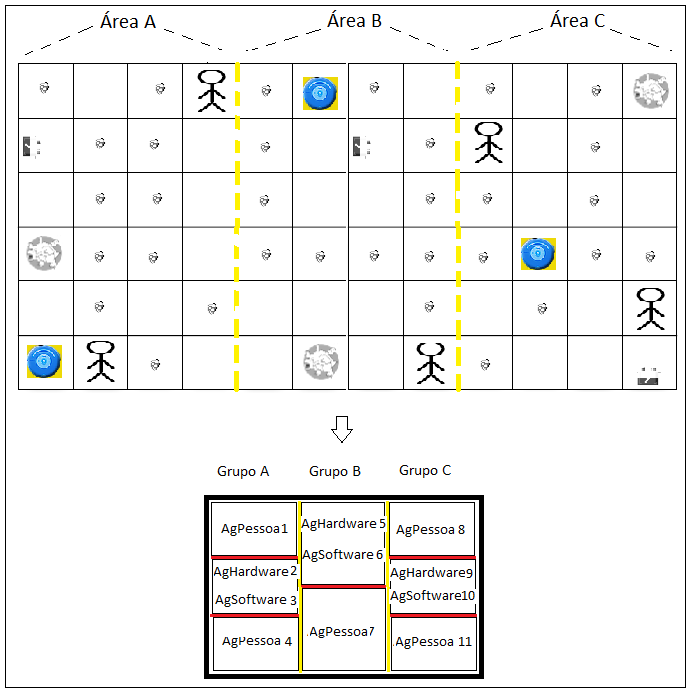
\includegraphics[width=8cm]{figuras/asp-estrutura.png}
        }{
            \Fonte{Elaborado pelo autor.}
        }   
    \end{figure}
    
    A Tabela \ref{tab:org-estrutura} apresenta o modelo $E$ para a organização esboçada na Figura \ref{fig:asp-estrutura}. Ela mostra um conjunto de onze programas de agentes, divididos em três grupos, cada grupo responsável por uma área do ambiente. A tabela apresenta apenas algumas relações do tipo Conhecimento, omitindo-se as relações de Controle, Coordenação e Autoridade existente entre os papéis que podem ser exercidos pelos programas.
    
    \begin{table}[h!]   
        \centering
        \Caption{\label{tab:org-estrutura} Organização dos agentes de acordo com o modelo de estrutura.}
        \UECEtab{}{
            \begin{tabular}{| p{5cm} | p{10cm}|}
            \hline
            \textbf{Agent} & \{$AgPessoa_1$, $AgHardware_2$, $AgSoftware_3$, $AgPessoa_4$, $AgHardware_5$, $AgSoftware_6$, $AgPessoa_7$, $AgPessoa_8$, $AgHardware_9$, $AgSoftware_{10}$, $AgPessoa_{11}$\} \\ \hline
            
            \textbf{Roles} & \{User, Device, Controller\}                                       \\ \hline
            
            \textbf{AgentRoles} & \{AgentAmIUser, AgentAmIDevice, AgentAmIController\}   \\ \hline
            
            AgentAmIUser & \{$AgPessoa_1$, $AgPessoa_4$, $AgPessoa_7$, $AgPessoa_8$\}   \\ \hline
            
            AgentAmIDevice & \{$AgHardware_2$, $AgHardware_5$, $AgHardware_9$\}         \\ \hline
            
            AgentAmIController & \{$AgSoftware_3$, $AgSoftware_6$, $AgSoftware_{10}$\}  \\ \hline
             
              
            \textbf{Groups} & \{\{$AgPessoa_1$, $AgHardware_2$, $AgSoftware_3$, $AgPessoa_4$\}, \{$AgHardware_5$, $AgSoftware_6$, $AgPessoa_7$\}, \{$AgPessoa_8$, $AgHardware_9$, $AgSoftware_{10}$, $AgPessoa_{11}$\}\} \\ \hline 
            
            \textbf{Bond} & \{$Bond_{knowledge}$(AgentAmIUser, AgentAmIDevice), \newline $Bond_{knowledge}$(AgentAmIDevice, AgentAmIController)\}    \\ \hline
            
             $Bond_{knowledge}$(AgentAmIUser, AgentAmIDevice) & \{($AgPessoa_1$, $AgHardware_2$), ($AgPessoa_4$, $AgHardware_2$), ($AgPessoa_7$, $AgHardware_5$), ($AgPessoa_8$, $AgHardware_9$), ($Agpessoa_{11}$, $AgHardware_9$), \dots \};  \\ \hline
        
             $Bond_{knowledge}$(AgentAmIDevice, AgentAmIController) & \{($AgHardware_2$, $AgSoftware_3$), ($AgHardware_5$, $AgSoftware_6$), ($AgHardware_9$, $AgSoftware_{10}$)\}  \\ \hline
             
             \vdots & \vdots \\ \hline

            \textbf{Communication} & \{($AgPessoa_1$, $AgHardware_2$), ($AgPessoa_1$, $AgHardware_5$), ($AgHardware_2$, $AgSoftware_3$), ($AgHardware_2$, $AgPessoa_4$), ($AgHardware_2$, $AgHardware_5$), ($AgHardware_2$, $AgPessoa_7$), \ldots \} \\ \hline
            
            \textbf{Frequency} & Ilustrado na Figura \ref{fig:matriz-decomponivel} \newline \\

            \hline
            \end{tabular}
        }{
        \Fonte{Elaborado pelo autor}
    }
    \end{table}
    
    
    Os programas de agentes $AgPessoa_1$, $AgPessoa_4$, $AgPessoa_7$, $AgPessoa_8$ e $AgPessoa_{11}$ são programas empregados para representar pessoas. Estes agentes exercem o papel de usuários do prédio (\textit{User}), que são capazes de caminhar em direção a qualquer local desejado. 
    
    Os programas de agentes $AgHardware_2$, $AgHardware_5$ e $AgHardware_9$, são programas empregados para representar o hardware dos sistemas técnicos no sistema \acrshort{ami}. Estes programas exercem o papel de sensores e/ou de atuadores (\textit{Devices}), capazes de perceber o ambiente, movimentar um aspirador e aspirar sujeira, além de interagir com os programas do tipo $AgPessoas$.
    
    Os programas de agentes $AgSoftware_3$, $AgSoftware_6$ e $AgSoftware_{10}$ são programas que implementam os componentes do software no sistema técnico do sistema \acrshort{ami}. Estes programas exercem o papel de controladores (\textit{Controller}) capazes de interagir com os agentes $AgHardware$, requisitando informações dos sensores e indicando ações adequadas para serem executadas pelos atuadores no ambiente.
    
    A segunda parte do modelo $E$, foca no componente da estrutura organizacional que descreve formalmente o mapa das interações entre os agentes na organização. Este mapa contém dois tipos de informações: (1) a relação $Communication$ na Tabela \ref{tab:org-estrutura} informa quem pode enviar mensagem para quem, dentro de um mesmo grupo e entre grupos diferentes de programas de agentes na organização; (2) a matriz sociométrica $Frequency$, ilustrada na Figura \ref{fig:matriz-decomponivel}, informa a frequência com que os programas de agentes trocam mensagens entre si, isto é, que em geral é necessária para dar suporte às relações binárias existentes entre os programas (Conhecimento, Controle, Coordenação e Autoridade) em diferentes papéis na organização. 
        
    \begin{figure}[h!]
        \centering
        \Caption{\label{fig:matriz-decomponivel} Mapa das interações entre os programas de agentes de diversos grupos.} 
        \UECEfig{}{
            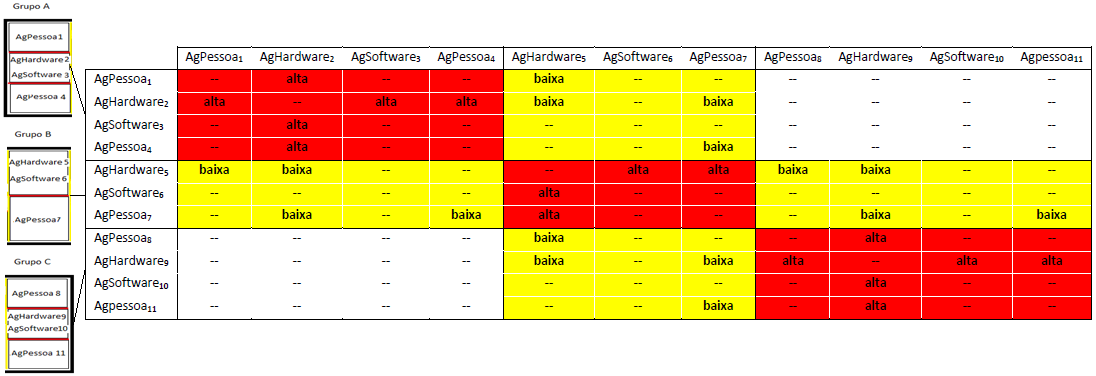
\includegraphics[width=12cm]{figuras/matriz-decomponivel.png}
        }{
            \Fonte{Elaborado pelo autor.}
        }   
    \end{figure}
    
    A matriz sociométrica acima informa a frequência $f_{xy}$ com que cada par de programas de agentes $(AgentAmI_x, AgentAmI_y) \in Communication$ trocam mensagens entre si. A matriz permite informar também as concentrações de interações densas, isto é, programas de agentes em um mesmo grupo estão agrupados na matriz, de forma que as células que possuem os maiores de valores de frequência ficaram numa linha de submatrizes quadradas ao longo da diagonal principal, e todos as células fora destes quadrados da diagonal têm valores de frequência zero ou muito pequeno.    
    
    Neste tipo de estrutura organizacional quase-decomponível, é possível distinguir as troca de mensagens entre grupos de agentes (amarelo) e as trocas dentro dos grupos (vermelho). Nestas organizações, as trocas de mensagens entre grupos são menos frequentes, mas não são desprezíveis. Assim, se dois agentes $AgentAmI_x$ e $AgentAmI_y$ estiverem em um mesmo grupo e existir uma “parede” comum entre eles então a frequência da troca de informações entre eles será: $f_{xy} = alta$. E se os agentes estiverem em grupos diferentes e existir uma parede separando-os então a frequência será $f_{xy} = baixa$ (ou, dependendo do caso, $f_{xy} = media$).
    
    Assim, considerando que a maioria dos sistemas \acrshort{ami} podem ser descritos por organizações de programas de agentes em uma estrutura quase-decomponível, o projetista pode agir de duas maneiras diferentes considerando as ideias implícitas no modelo E. Ele pode empregar a primeira parte do modelo para formalizar previamente os grupos de agentes na organização e, em seguida, empregar a segunda parte do modelo para formalizar o mapa de interações sociais em função dos grupos formalizados. Mas ele pode também, formalizar previamente o mapa de interações entre os agentes e, em seguida, formalizar os grupos operacionalmente considerando uma medida de frequência de interação no mapa. 
    
    
    \subsection{Modelo de Comportamento (C)}
    
        Depois de se concentrar na descrição estrutural empregando o modelo $E$ da organização de programas de agentes representando o sistema \acrshort{ami}, o projetista deve ser capaz de descrever como a estrutura projetada deve funcionar (comportamento) para realizar o objetivo original do sistema, sua função descrita no modelo $F$, no ambiente de tarefas. O modelo de comportamento (modelo $C$) permitirá à descrição formal de procedimentos de tomada de decisão nos programas de agentes, em seus papéis na organização e nos processos que ocorrem dentro da organização. Definindo como os programas de agentes, integrados na estrutura organizacional, devem agir de maneira a alcançar os resultados desejados.
        
        O quadro formal que define o modelo $C$ pode ser dividido em duas partes. A primeira parte permitirá ao projetista definir os “esqueletos” dos programas de agentes, definidos no conjunto $Agents$ do modelo $E$. Estes esqueletos de programa deverão ser customizados de acordo com os papéis assumirão em um domínio específico de aplicação. Essa customização implica na definição do conjunto de comportamentos que cada programa deve ser capaz de executar quando adotar algum papel na organização, no modelo $E$ aqueles papéis definidos no conjunto $Roles$. A segunda parte do quadro permitirá ao projetista definir o protocolo de interação descrevendo as trocas de mensagens possíveis, no modelo $E$ descritas na relação $Communication$, visando coordenar as ações dos programas em seus papéis na organização.
        
        \subsubsection{Descrição Formal dos “Esqueletos” de Programas de Agentes}
        
            No nível individual, o modelo $C$ permitirá ao projetista descrever formalmente os esqueletos dos programas de agentes na organização. Cabe ao projetista definir a especificação do conjunto de comportamentos a serem incorporados nesses esqueletos. Que devem ser adequados aos papéis $R_j \in Roles$ que os programas nos conjuntos $AgentAmIRj \in AgentRoles$, descritos no modelo $E$, devem assumir no domínio de aplicação de interesse do projetista. O formalismo para descrição destes esqueletos, foi sintetizado a partir dos trabalhos de \citeonline{norvig2004inteligencia} sobre estruturas de programas de agentes, e de \citeonline{wooldridge2009introduction} sobre arquiteturas abstratas de agentes. A Figura \ref{fig:estrutura-agente} ilustra graficamente a estrutura e os esqueletos de pelo menos quatro tipos diferentes de programas de agentes resultantes desta síntese.
            
            Mais especificamente, a figura ilustra um refinamento em duas etapas do subsistema de tomada de decisão, $ação: S^*  \rightarrow A$ (função que mapeia sequências de estados do ambiente $s \in S^*$ em ações $a \in A$), apresentada na seção que descreve o quadro formal associado ao modelo $F$ da organização. À esquerda, o primeiro refinamento dando origem ao subsistema de percepção do agente. À direita, o segundo refinamento dando origem ao subsistema de estado interno do agente. O primeiro refinamento apresenta a arquitetura e o esqueleto de programas de agentes reativos simples baseados em regras condição-ação. O segundo refinamento apresenta a arquitetura e o esqueleto de programas de agentes reativos baseados em modelos, orientado por objetivos e orientados por metas, dependendo do tipo de informação ($InfoDecisão$) que o projetista desejar incorporar no processo de tomada de decisão (regras, objetivo, utilidade).
            
            \begin{figure}[h!]
                \centering
                \Caption{\label{fig:estrutura-agente} Estrutura dos programas de agente.} 
                \UECEfig{}{
                    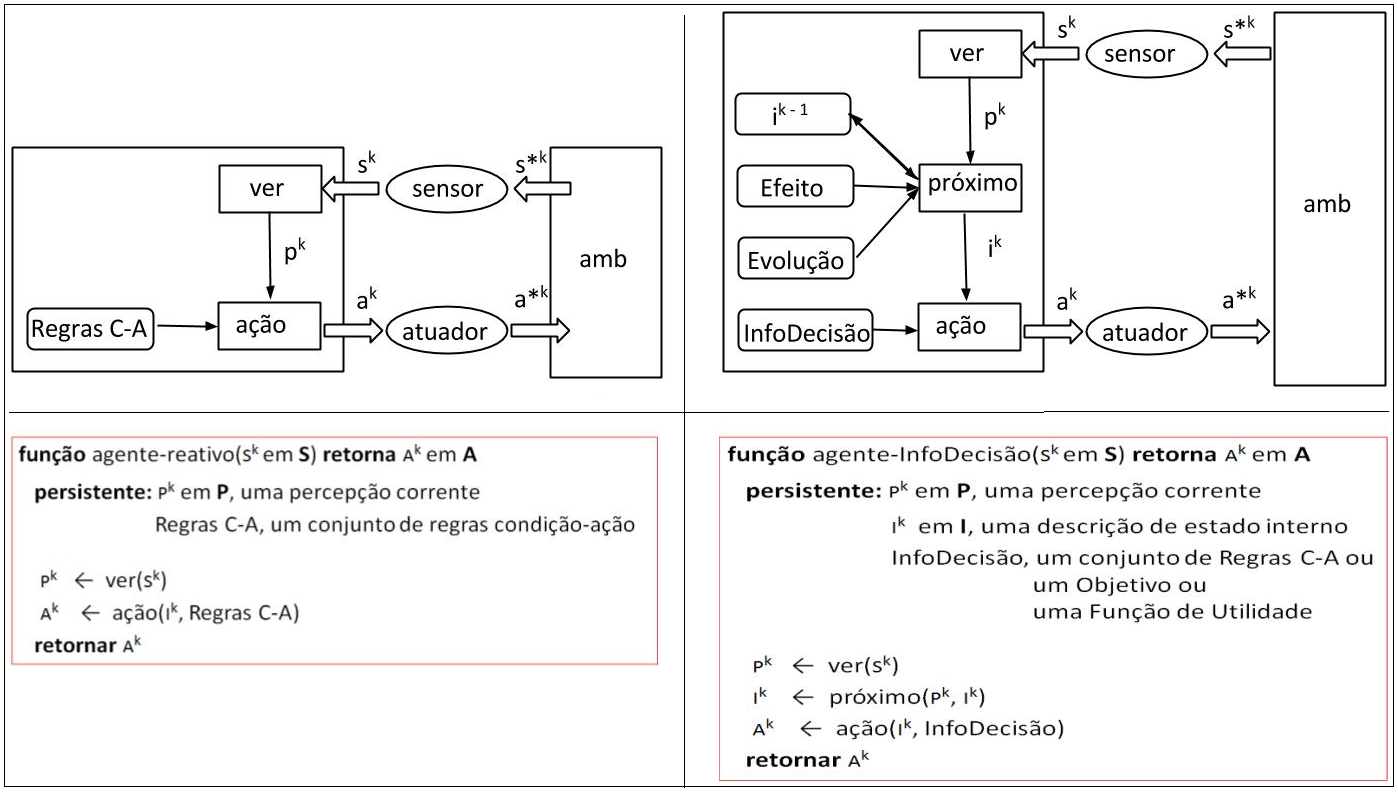
\includegraphics[width=12cm]{figuras/estrutura-agente}
                }{
                    \Fonte{Elaborado pelo autor.}
                }   
            \end{figure}
            
            Além de serem empregados na concepção de programas de agentes para representar pessoas e o software do sistema. Esses esqueletos devem ser utilizados também na concepção de programas de agentes, para representar o hardware do sistema. Esses agentes são ilustrados na Figura \ref{fig:estrutura-agente} como elipses, com os nomes sensor e atuador, conforme ilustram os esqueletos de agentes reativos simples empregados para representar estes componentes do hardware nos sistemas técnicos ilustrados na figura na Figura \ref{fig:org-level-p4}. O quadro abaixo consiste em uma extensão do quadro inicialmente desenvolvido no modelo $F$, o mesmo apresenta o esquema de representação e a definição correspondente dos principais termos envolvidos na definição dos esqueletos de programas de agentes ilustrados na Figura \ref{fig:estrutura-agente}.
            
            \begin{table}[h!]   
            \centering
            \Caption{\label{tab:def-prog-agent} Definição dos termos envolvidos no esqueleto do programa de agente.}
            \UECEtab{}{
                \begin{tabular}{| p{4cm} | p{10cm}|}
                \hline
                $P = \{P_1, P_2, \ldots \}$ & Percepção do ambiente do agente - em qualquer instante o agente recebe por meio de sensores entradas perceptivas em um conjunto de percepções do ambiente;\\ \hline
                
                $ver: S  \rightarrow P$ & Subsistema de percepção do programa - captura a habilidade do agente observar seu ambiente, uma função que mapeia estados do ambiente para percepções;      \\ \hline
                
                $I = \{I_1, I_2, \ldots \}$ & Estados internos do ambiente - em qualquer instante o agente mantém em memória uma descrição de estado em um conjunto de estados interno do ambiente;   \\ \hline
                
                próximo: $I\times P \rightarrow I$ & Subsistema de atualização de estado interno do programa – função que mapeia um estado interno e a percepção atual, que chega da função ver, em um estado interno;   \\ \hline
                
                ação: $I \rightarrow A$ & Subsistema de tomada de decisão do programa – função que mapeia estados internos em ações.         \\ \hline
                
                $Sucessor: I \rightarrow P(I \times A)$ & Efeito das ações do agente no ambiente – função que mapeia um estado interno em um conjunto de pares estado interno e ação;   \\ \hline
                 
                Ações: $I \rightarrow 2^A$ & Conjunto de ações possíveis para o agente em um estado – mapeia um estado interno em um conjunto de ações possíveis de serem executadas no estado;  \\ \hline
                
                $RESULTADO: I \times A \rightarrow I$ & Modelo de transição – descrição formal do que cada ação faz, uma função que mapeia um estado interno e uma ação em um novo estado interno; \\ \hline
            
                Meta:$I \rightarrow \{V,F\}$ & Função que mapeia uma descrição de estado interno em um valor verdade;  \\ \hline
                 
                $Utilidade: I \rightarrow \mathbb{R}$ & Função que mapeia uma descrição de estado interno em um valor real. \\ 
                \hline
                \end{tabular}
            }{
            \Fonte{Elaborado pelo autor}
        }
        \end{table}
        
        Em resumo, à esquerda na Figura \ref{fig:estrutura-agente}, um programa agente reativo simples seleciona suas ações baseando-se apenas em sua percepção atual e em um conjunto de regras no formato condição-ação. À direita na Figura \ref{fig:estrutura-agente}, um programa agente reativo baseado em modelos mantém internamente em memória uma descrição de estado de seu ambiente, o qual depende do histórico de suas percepções. Essa mesma figura pode representar um programa agente orientado por objetivos, que além das informações em memória, considera a informação sobre os objetivos que descrevem situações desejadas no ambiente. O programa do agente orientado por utilidade possui uma função utilidade que mapeia uma descrição de estado do ambiente em um grau de felicidade associado. 
    
        O subsistema de atualização de estado interno (próximo) dos agentes reativos baseados em modelos, orientados por objetivos e por utilidade. E o subsistema de tomada de decisão (ação) dos dois últimos, em comum, processam informações de dois tipos, ou seja: sobre como ambiente evolui independentemente das ações do agente (Evolução) e sobre o efeito das ações do agente no ambiente (Efeito). A utilização destas informações nos dois subsistemas pode ser representada por meio de uma função Sucessor de estado, e/ou por meio das funções \emph{Ações} e \emph{RESULTADO} no quadro.
        
        As informações sobre o objetivo, processadas pelo subsistema de tomada de decisão do agente orientado por objetivo, é representada por um teste Meta. Quando verdadeiro, este teste diz ao agente que ele pode parar o seu processo de deliberação. De forma semelhantemente, o agente orientado por utilidade deve empregar uma função utilidade, do tipo especificado no modelo $F$, para medir a qualidade dos estados realizados por ações que ele tenha como alternativas.
        
        O algoritmo \ref{alg:decision-function} descreve uma da função tomada de decisão um programa de agente aspirador de pó, do tipo $AgSoftware$ no papel Controlador. O programa deve ser capaz de controlar o aspirador visando varrer uma área e aspirar aqueles locais que contém sujeira. O aspirador deve realizar um movimento horizontal (direita ou esquerda) na área enquanto não perceber sujeira e obstáculos. Quando perceber que existe um obstáculo (parede ou pessoa), impossibilitando-o de realizar um movimento, o aspirador deve realizar um movimento vertical para cima/baixo (girar $90^\circ$ no sentido anti-horário e seguir em frente). Em seguida, modificar a direção horizontal (esquerda/direita e vice-versa) e seguir em frente em busca de novos locais contendo sujeira.
        
        \begin{algorithm}[h!]
            %\SetSpacedAlgorithm
            \caption{\label{alg:decision-function} Descrição parcial da função tomada de decisão de um agente reativo.}
            %\Entrada{$p^k$ em S}
            %\Saida{$a^k$ em A}
            função ação ($p^k$ em S) retorna $a^k$ em A\\
            \Inicio{
                \ldots\\
                \textbf{se} $p^k$ = obstaculo \textbf{então} \textbf{retornar} $a^k$ = aspirar\;
                \textbf{senão se} $p^k$ = obstaculo \textbf{então} \textbf{retornar} $a^k$ = rotacionar $90^\circ$ esquerda\;
                \textbf{senão se} $p^k$ = limpo \textbf{então} \textbf{retornar} $a^k$ = frente\;
                \ldots\\
            }
        \end{algorithm}
        
        A função tomada de decisão diz respeito a um programa de um agente do tipo reativo simples baseado em regras condição ação. As expressões que definem as condições nas regras são estabelecidas levando-se em consideração as informações no conjunto de percepções do ambiente que são possíveis para o agente, $P = \{P_1, P_2, \ldots \}$. Os programas de agentes baseados em modelos são mais adequados para ambientes parcialmente observáveis. Eles podem empregar as informações que descrevem o estado interno, $I = \{I_1, I_2, \ldots \}$, para evitar retornar em locais por onde já passaram. E ainda evitar passar em locais que foram visitados recentemente por outros agentes, através de um processo cooperativo de troca de mensagens em um sistema composto por mais de um aspirador.
    
    \subsubsection{Descrição Formal do Protocolo de Interação Global Entre os Agentes}
    
        Na subseção anterior descrevemos a parte do modelo $C$ que representa o comportamento interno de um agente. Mas essa parte do modelo só é capaz de descrever sistemas que contenham agentes únicos. Em vez de um sistema \acrshort{ami} formado por um único aspirador, vale considerar a situação em que um grupo de aspiradores são capazes de cooperar uns com os outros. Os agentes podem trocar mensagens contendo informações úteis sobre o ambiente de tarefas, visando alcançar da melhor maneira o objetivo original do sistema. 
        
        O processo de comunicação e intercâmbio de conhecimento é conhecido como cooperação. Dependendo do ambiente de tarefas, a cooperação pode ser um requisito crucial. Por exemplo, cada agente pode cooperar utilizando a operação coletiva \textit{broadcast}, ou seja, de transmissão de uma mesma mensagem para todos os outros agentes no grupo. 
    
        A ideia é que para alcançar seus objetivos e o objetivo original do sistema, os agentes componentes possam se comunicar através de uma linguagem de comunicação em que os atos de fala são visualizados como ações (da mesma forma que as ações executadas pelos atuadores do agente), cujos efeitos ocorrem principalmente nos modelos que os falantes e os ouvintes mantêm uns dos outros. Neste contexto, os atos de fala dos agentes podem ser integrados nos processos de atualização de estado interno (informação sobre efeito de um ato) e de tomada de decisão dos programas de agentes (por exemplo, como consequentes em regras condição-ação). 
        
        A segunda parte do modelo $C$ foca na descrição do quadro formal, que pode ser adaptado para definir o protocolo de comunicação entre os agentes em um mesmo grupo e entre os agentes em grupos diferentes na organização. A abordagem considera que os agentes são capazes de trocar mensagens por meio de canais de comunicação. Cada agente atua assincronamente monitorando uma fila de mensagens de entrada, que chegam pelo canal, e enviando mensagens para uma fila de saída, que serão transmitidas pelo canal para um ou mais agentes.
        
        A principal parte do quadro proposto para a segunda parte do modelo $C$, consiste em uma variação do quadro empregado para a definição formal da noção de autômatos de estados finitos (\acrshort{afd}). O quadro resultante empresta algumas ideias implementadas no formalismo para a especificação de cenas em instituições eletrônicas \cite{vasconcelos2002approach}, baseado na noção de autômatos finitos não determinísticos. No modelo $C$, um protocolo de interação entre agentes é descrito como um \acrshort{afd}. Onde os estados representam diferentes estágios de conversação e os arcos direcionados conectando os estados são rotulados com mensagens escritas em uma linguagem de comunicação, ou com alguma condição descrita em termos de um período de tempo entre dois instantes consecutivos de transmissão de mensagens no processo de conversação. Ou seja:
        
        \newtheorem{theorem}{Definição}

        
        \begin{theorem}
            Protocolo = $(T, LC, Q, q_0, \delta, G)$, tal que:
            \begin{itemize}
                \item T = \{$t_1$, \ldots, $t_m$\} - um conjunto discreto e parcialmente ordenado de instantes, para marcar a transmissão de mensagens em um processo de conversação;
                \item LC – linguagem empregada para a comunicação entre os agentes;
                \item Q – conjunto de estados possíveis do protocolo (é finito);
                \item $q_0 \in Q$ – estado inicial do protocolo;
                %\item $F \subset Q$ - conjunto de estados finais do protocolo; % NAO EXISTE MAIS
                \item $\delta$ – função programa ou função transição (função parcial) – associa estados em $Q$ e mensagens em $LC$, ou uma condição descrita em termos de T, a estados em $Q$, ou seja, $\delta$: $Q$ $\times$ ($LC$ $\cup$ condição(T)) $\to$ $Q$;
                \item $G \subset P(Agentes)$ – família de conjuntos de agentes que podem participar do processo de conversação especificado no protocolo.
            \end{itemize}
        \end{theorem}
        
        A especificação de um protocolo de comunicação entre um grupo de agentes $G$ considera um único estado inicial $q_0$. Apesar de não existirem estados finais, o estado inicial também representa as diferentes possibilidades de um agente finalizar uma conversação. Com relação à linguagem para comunicação ($CL$), o modelo $C$ considera uma linguagem de atos de fala que podem ser gerados a partir de dois atos de fala considerados como mensagens fundamentais: $request$ e $inform$. A Figura \ref{fig:inform-request} ilustra o formato proposto para estas mensagens e dois exemplos de composições destas mensagens visando gerar atos de fala de perguntas (\textit{requests to inform}) e solicitações envolvendo pelo menos três agentes (\textit{requests to request}). 
    
        \begin{figure}[h!]
            \centering
            \Caption{\label{fig:inform-request} Troca de mensagens entre os agentes da organização.} 
            \UECEfig{}{
                \includegraphics[width=8cm]{figuras/inform-request}
            }{
                \Fonte{Elaborado pelo autor.}
            }   
        \end{figure}
            
        Cada mensagem transmitida deve conter representações de informações sobre a intenção da mensagem dos agentes falantes ($S$) e os ouvintes ($H$). Assim como sobre o conteúdo da mensagem a ser trocado entre os agentes ($Action$ ou $Statement$) e o instante ($t$) da conversação. Qualquer agente falante $S$ que envia uma mensagem do tipo $request$, objetiva fazer com que algum agente ouvinte $H$ execute uma ação $Action$. Qualquer agente falante $S$ que envia uma mensagem do tipo $inform$, objetiva fazer com que o agente ouvinte $H$ acredite em alguma afirmação ($Statement$). Assim como no caso da fórmulação de mensagens envolvendo questões, toda a semântica dos atos de fala que compõem a linguagem de comunicação \acrshort{fipaacl} (\acrlong{fipaacl}) pode ser definida em termos de $inform$ e $request$.
        
        Para ilustrar a formalização da noção de protocolos, vale considerar o exemplo do grupo de aspiradores capazes de cooperar uns com os outros, visando limpar o ambiente no menor tempo possível. Por exemplo, cada agente pode cooperar utilizando a operação coletiva \textit{broadcast}, transmitindo uma mesma mensagem para todos os outros agentes no grupo. Assim, quando perceber um local (célula) contendo sujeira, o agente pode transmitir a posição da célula e a quantidade de sujeira aos outros. Quando a mensagem for recebida, cada agente pode armazenar as informações no estado interno e, em seguida, decidir se vai em direção ao local, avisando ou não ao agente que enviou a mensagem. Quando limpar uma célula, o agente pode transmitir esta informação novamente para os outros agentes no grupo. Quando a mensagem for recebida, o agente pode remover do estado interno a informação sobre sujeira na célula que foi limpa.
        
        A Figura \ref{fig:protocolo-transicao} descreve graficamente uma parte da função transição ($\delta$) componente do protocolo de comunicação entre os agentes. O protocolo considera um conjunto de dois estados possíveis, $Q$ = \{$q_0$, $q_1$\}, com o estado inicial representado por $q_0$. A figura supõe que o processo de conversação envolve uma família formada por um conjunto contendo os programas no papel Controller, isto é, G = {AgentAmIController} (como G é unitário, em vez de fazer referência ao conjunto AgentAmIController, a figura faz referência à própria família G).
            
        \begin{figure}[h!]
            \centering
            \Caption{\label{fig:protocolo-transicao} Protocolo de transição.} 
            \UECEfig{}{
                \includegraphics[width=8cm]{figuras/protocolo-transicao}
            }{
                \Fonte{Elaborado pelo autor.}
            }   
        \end{figure}
       
        Na primeira etapa do processo de conversação, no instante $t_1$, representada pelo componente da função transição $\delta$($q_0$, $inform(\ldots, t_1)) = q_1$, um agente falante s $\in$ G pode enviar sua posição ($x_1$, $y_1$) e a quantidade de sujeira z na posição para todos os outros agentes ouvintes h $\in$ G. Na segunda etapa, no instante $t_2$, alguns dos agentes ouvintes podem responder a mensagem dizendo se definiram, ou não, a posição ($x_1,y_1$) como meta, $\delta$($q_1$, $inform(\ldots, t_2) = q_0$. Entretanto, os agentes podem não enviar mensagem de retorno. Neste caso, depois de $\epsilon$ unidades de tempo, contadas a partir do horário de início da conversação no instante $t_1$ (tempo($t_1$)) até um tempo limite em que uma mensagem de retorno deve ser enviada no instante $t_2$ (tempo($t_2$)), o protocolo transita para o estado inicial, $\delta$($q_1$, tempo($t_2$) – tempo($t_1$) > $\epsilon$, $t_2$) = $q_0$, em que os agentes poderão iniciar novo processo de conversação.
        
        Conforme ilustra o mapa das iterações sociais na Figura \ref{fig:matriz-decomponivel}, a descrição parcial da função transição omitiu as trocas de mensagens que existem entre os agentes no papel $AgentAmIDevice$ e os agentes no papel $controller$. Estas trocas ocorrem com muita frequência e, assim como possíveis trocas entre os agentes no papel $AgentAmIDevice$ com os agentes no papel $AgentAmIUser$   , devem ser especificadas de maneira a completar a definição do protocolo de interação global entre todos os agentes no grupo exemplificado.
        
\end{section}

\section{Considerações Finais}

    A proposta \textbf{P6}, escrita na introdução deste capítulo, consiste na utilização de simulação computacional baseada em agentes (\acrshort{ads}) como um meio para examinar a dinâmica de um sistema \acrshort{ami}. A \acrshort{ads} permitirá ao projetista experimentar diversos contextos operacionais do sistema \acrshort{ami}. Possibilitando a aquisição de novos conhecimentos sobre o funcionamento do sistema em seu ambiente. E outras formas de adaptar o seu modelo estrutural ($E$) e o comportamental ($C$),  visando melhorar o desempenho do sistema quando for necessário, de acordo com o que for especificado no modelo $F$.
    
    Conforme a Figura \ref{fig:sim-emergente-p6} (na seção de introdução deste capítulo) indica, a execução de uma simulação considera como informações de entrada, o modelo \acrshort{fec} do sistema \acrshort{ami}, o modelo do ambiente de tarefas e os valores dos parâmetros de entrada. Descrevendo um contexto operacional de funcionamento do sistema no ambiente. A execução de uma \acrshort{ads} deve gerar como saída, as informações sobre o desempenho do sistema conforme descrito no modelo $F$. Essas informações de desempenho, ou objetos emergentes, são resultado das interações descritas no modelo $C$. Executadas por programas de agentes na organização estruturada no modelo $E$. 
    
    Uma execução pode ser vista como uma dedução de alguma informação sobre o sistema \acrshort{ami} sendo projetado. Uma coleção destas deduções, obtidas metodicamente pela execução de várias \acrshort{ads}, pode ser vista como a informação necessária para o projetista realizar inferências (indutivas) sobre o comportamento do sistema. Permitindo a ele deduzir se o sistema será capaz de realizar o objetivo original em seu ambiente de tarefas.
    
	\chapter{Aplicação exemplos}
\label{cap:resultados}

\lstdefinelanguage{NetLogo}{
	morekeywords=[1]{to,to-report,end, extensions,to-report,globals,breed,directed-link-breed, link-breed},
	extendedchars=true, 
    breaklines=true,
    breakatwhitespace=true,
    basicstyle=\ttfamily,
    columns=fullflexible,
	tabsize=4,
    keywordstyle=[1]\color[rgb]{0.25,0.5,0.35},%\color[rgb]{0.4,0.8,0.2}\bfseries,
    morekeywords=[2]{let,set,loop, if, report, foreach, print, tick, while, every, ifelse, ask},
    keywordstyle=[2]\color{blue},
    alsoletter={-,?,.},
    morekeywords=[3]{position, not, reverse, fput, substring, length, word, timer,is-number?,filter,first, bf, butfirst, last, empty?, n-of, color, who, shape},
    keywordstyle=[3]\color[rgb]{0.6,0,0.8},
    comment=[l]{\;},
    commentstyle=\color[rgb]{0.75,0.75,0.75},
    string=[d]{"},
    stringstyle=\color{orange},
    otherkeywords={1, 2, 3, 4, 5, 6, 7, 8, 9, 0},
    morekeywords=[4]{1, 2, 3, 4, 5, 6, 7, 8, 9, 0, true, false},
    keywordstyle=[4]{\color{orange}},
}


Este capítulo apresenta uma primeira aplicação da abordagem proposta no capítulo anterior para o projeto de sistemas de inteligência ambiental (sistemas \acrshort{ami}). Conforme mencionado, a abordagem consiste em uma contribuição para a etapa de análise funcional do sistema e no \textit{feedback} que ela pode dar para refinar a análise de requisitos e a síntese do projeto. O domínio de aplicação da ideia escolhido pertence à área de pesquisa e desenvolvimento tecnológico resultante da combinação da robótica autônoma e da inteligência ambiental, mais especificamente o campo dos robôs aspiradores de pó.

Apesar do domínio de aplicação específico como o mundo dos aspiradores de pó, o capítulo visa mostrar aos projetistas, de sistemas AmI em geral, como projetar estes sistemas em termos de modelos \acrshort{fec} associados e como realizar estudos experimentais objetivando verificar/encontrar decomposições funcionais alternativas de subsistemas componentes, capazes de atender aos requisitos funcionais e de desempenho dos sistemas AmI. O ambiente de tarefas e os programas dos agentes representando as pessoas e os robôs aspiradores de pó foram implementados em NetLogo \cite{wilensky1999netlogo}, uma plataforma de software que facilita o desenvolvimento das capacidades dos programas dos agentes e do dinamismo do ambiente. A razão para a escolha dessa plataforma é alta simplicidade em representar os agentes, facilitando a construção de ambientes complexos em curto espaço de tempo. Os codigos utilizados para construir a simulação podem ser observados no seguinte endereço \footnote{https://bitbucket.org/rob\_oliveira/netlogocleanersim}.

O capítulo foi dividido em mais quatro seções. A Seção \ref{sec:dom-aplicacao} descreve o domínio de aplicação, isto é, o sistema AmI pretendido e seu ambiente de tarefas. A Seção \ref{sec:cenario-teste} apresenta o cenário de teste adotado, as propriedades do ambiente de tarefas e as funcionalidades necessárias ao sistema neste ambiente. A Seção \ref{sec:plat-sim} apresenta os principais aspectos associados a plataforma de simulação NetLogo, que são importantes para a compreensão dos resultados. A Seção \ref{sec:dev-experimento} apresenta os projetos em modelos \acrshort{fec} e os resultados (objetos emergentes) de suas simulações na NetLogo.  E, finalmente, na seção \ref{sec:conclusao} discutimos os resultados obtidos nos experimentos. 

\section{Domínio de Aplicação}
\label{sec:dom-aplicacao}

O domínio proposto está dentro de uma combinação das áreas de robótica autônoma e de inteligência ambiental. De um lado, a robótica autônoma visando criar robôs compostos por sensores, atuadores e controladores, que sejam capazes de viver em casas e locais públicos, e sejam habilidosos na realização de tarefas físicas que ajudem na vida cotidiana das pessoas. De outro lado, a inteligência ambiental visando criar redes de dispositivos domésticos inteligentes capazes de fornecer informações, comunicação e serviços para as pessoas. A Figura \ref{fig:dom-ami} ilustra um exemplo destes robôs autônomos em um ambiente de computação ubíqua inteligente, em que existem muitos computadores e redes sensores no ambiente para a geração de informações úteis para o controle dos robôs.

\begin{figure}[h!]
    \centering
    \Caption{\label{fig:dom-ami} Ilustração da ideia de inteligência ambiental e robôs autônomos} 
    \UECEfig{}{
        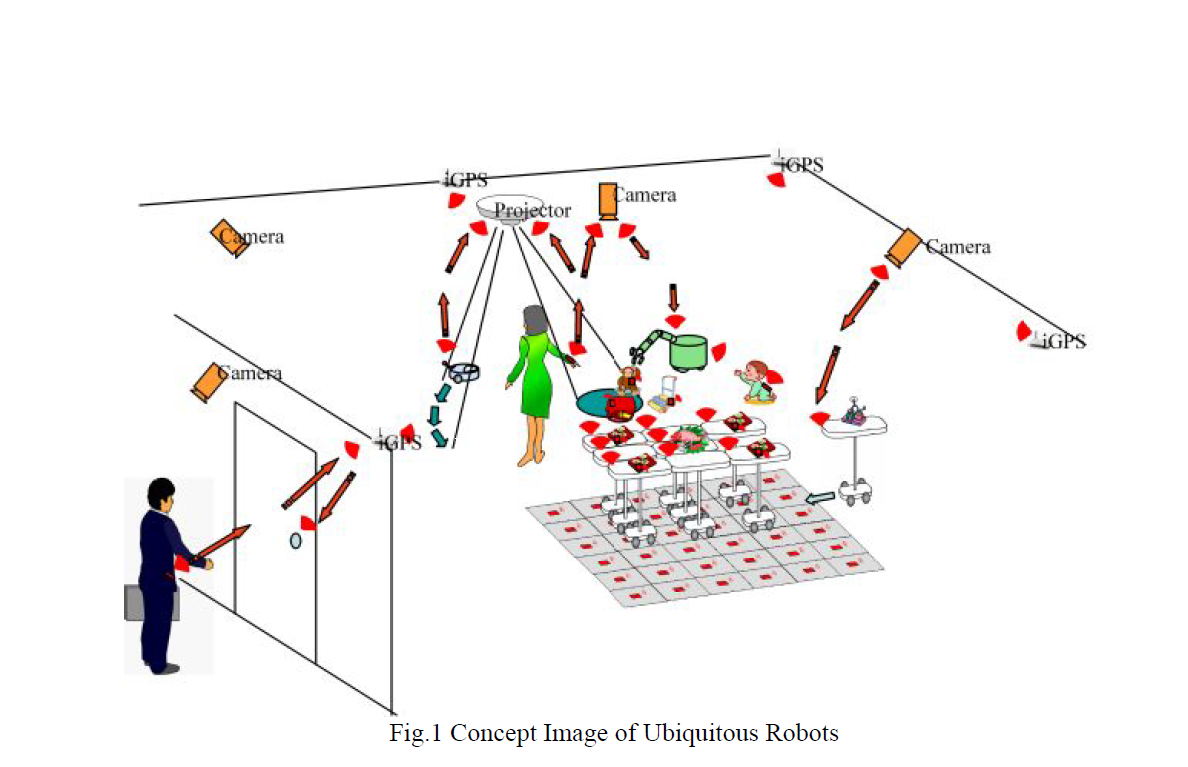
\includegraphics[width=8cm]{figuras/dom-ami}
    }{
        \Fonte{Elaborado pelo autor}
    }   
\end{figure}

Dentro do contexto da combinação da robótica autônoma e da inteligência ambiental, o sistema AmI para aplicação da abordagem envolve o campo dos robôs aspiradores de pó. Este tipo de robô faz parte do mundo atualmente conhecido como Internet das Coisas (\acrshort{iot}). O propósito de um robô aspirador é ser um servo para as pessoas, economizando o tempo e esforço, limpando a sujeira de locais de interesse. Por exemplo, a fabricante LG disponibiliza uma vasta gama de aparelhos inteligentes que são controlados por um aplicativo de mensagens. Em particular, esta empresa fabrica um robô aspirador denominado \textit{HomeBot Square}  (Figura \ref{fig:cleaner-bot}a). Através do aplicativo de mensagens, o \textit{HomeBot Square} e outros dispositivos inteligentes LG podem ser programados com comandos em linguagem natural.

\begin{figure}[h!]
    \centering
    \Caption{\label{fig:cleaner-bot} Aspiradores de pó inteligentes: HomeBot Square e Roomba 980} 
    \UECEfig{}{
        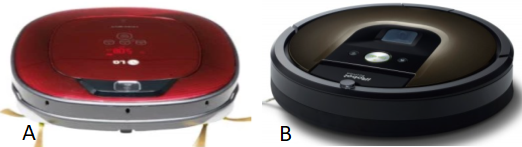
\includegraphics[width=8cm]{figuras/cleaner-bot.png}
    }{
        \Fonte{Elaborado pelo autor}
    }   
\end{figure}

A companhia iRobot fabrica o robô aspirador Roomba 980 (Figura \ref{fig:cleaner-bot}b). Conhecido como o aspirador da Internet das Coisas, o Roomba 980 pode ser controlado por meio de aplicativos. A companhia garante que o robô é capaz de executar suas tarefas em um tempo contínuo de duas horas, retornando automaticamente a sua base de carga e em seguida voltar ao trabalho até que o local pretendido esteja limpo. Roomba é capaz de limpar área abertas movendo-se em linhas paralelas, empregando um conjunto de sensores para adaptar este padrão quando necessário, navegando perfeitamente entre os móveis e a desordem. Essencialmente, a iRobot instalou uma câmera em cima do Roomba 980, a qual constantemente mapeia o local à medida que o robô se movimenta, tornando-o mais eficiente. 

\section{Cenário de Teste}
\label{sec:cenario-teste}

Para ilustrar a aplicação da abordagem, o cenário de teste considera um sistema técnico composto por um conjunto de agentes artificiais robôs aspiradores de pó responsáveis por limpar uma área quadrada (retangular) em um aeroporto, que pode conter obstáculos, sujeira e pessoas, distribuídas de maneira aleatória em uma área determinada. A Figura \ref{fig:ami-aplication} ilustra um cenário específico contendo um conjunto de quatro agentes artificiais, quatro usuários, três obstáculos, três pontos de recarga de energia e bastante lixo. 

\begin{figure}[h!]
    \centering
    \Caption{\label{fig:ami-aplication}Exemplo de um cenário de teste.} 
    \UECEfig{}{
        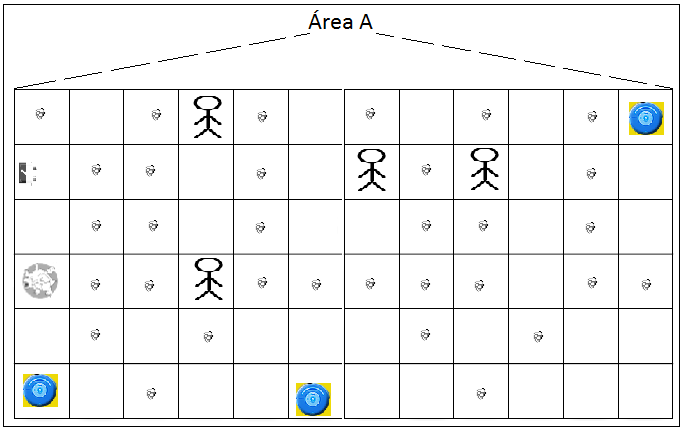
\includegraphics[width=8cm]{figuras/ami-aplication.png}
    }{
        \Fonte{Elaborado pelo Autor}
    }   
\end{figure}

O ambiente de tarefas é parcialmente observável e não determinístico, pois alguns atuadores dos robôs podem falhar. As pessoas que circulam pelo ambiente podem depositar sujeira pelos locais por onde passam, tornando o ambiente dinâmico. Uma configuração particular do ambiente pode ser definida considerando-se as quantidades de robôs, de obstáculos, de lixo e de pessoas em locais específicos do aeroporto. Diferentes configurações compreendem a diferentes cenários (casos) de teste, definindo problemas de diferentes níveis de dificuldade. Por exemplo, algumas configurações podem exigir dos robôs maior consumo de energia, enquanto que outras podem colocar lixo em locais de mais fácil acesso aos robôs. 

Neste tipo de ambiente difícil, cada agente artificial aspirador de pó deve ser capaz de perceber e atualizar seu conhecimento sobre o ambiente sempre que se mover, identificando e localizando cada um dos objetos, visando realizar o objetivo original do sistema, ou seja, limpar o máximo de sujeira possível, gastando o mínimo de energia e evitando obstáculos quando for necessário. Ele também deve ser capaz de cooperar com os outros agentes no ambiente, por meio de processos de comunicação e troca de conhecimentos úteis para a realização de seus objetivos e do objetivo original do sistema. Seção \ref{sec:dev-experimento} descreve em detalhes a funcionalidade de cada um dos agentes no cenário proposto. 


\section{Plataforma de Simulação}
\label{sec:plat-sim}

O ambiente de simulação e os programas dos agentes representando as pessoas e os robôs aspiradores de pó foram implementados em NetLogo \cite{wilensky1999netlogo}, uma plataforma de software que facilita o desenvolvimento das capacidades dos programas dos agentes e do dinamismo do ambiente. O ambiente é concebido como um recipiente em que existem objetos observáveis, incluindo obstáculos, lixo e pessoas. As propriedades dos objetos podem ser alteradas e novos objetos podem ser concebidos facilmente e inseridos no ambiente. A Figura \ref{fig:netlogo-env} ilustra um ambiente em tempo de execução. Neste ambiente, existe um agente aspirador de pó (vermelho), cinco obstáculos (marron) e uma grande quantidade de sujeira (cinza).


\begin{figure}[h!]
    \centering
    \Caption{\label{fig:netlogo-env}Simulação NetLogo: programa aspirador de pó em um ambiente de tarefas.} 
    \UECEfig{}{
        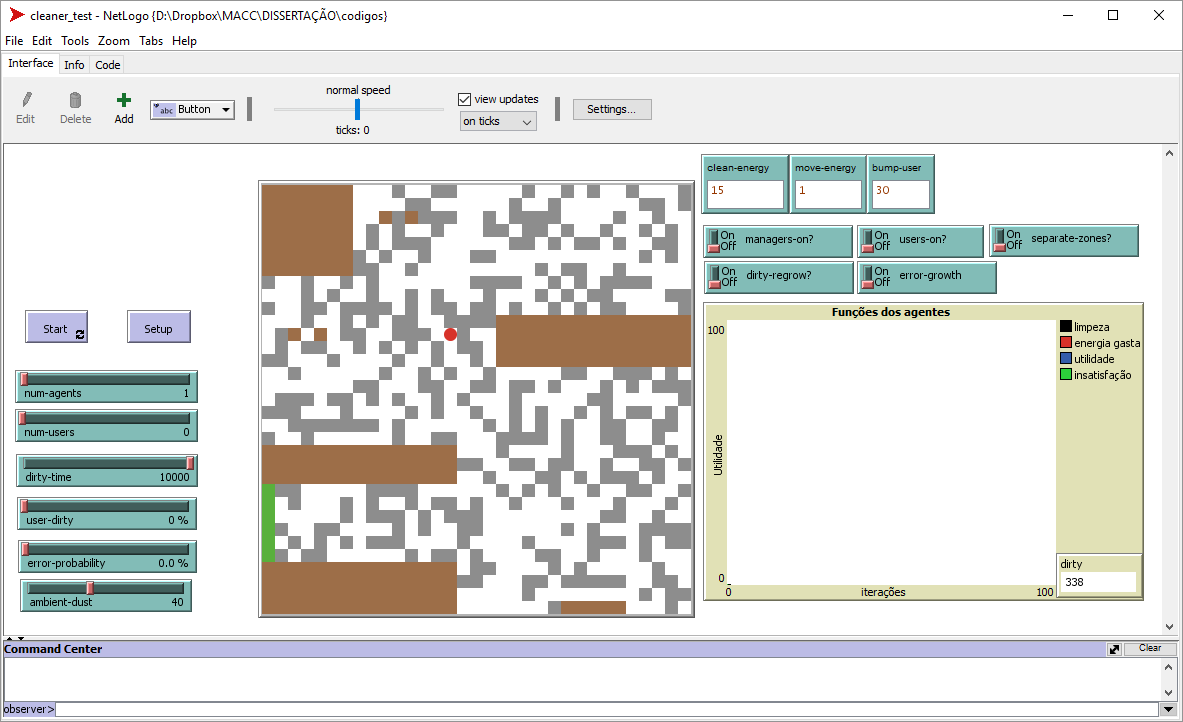
\includegraphics[width=10cm]{figuras/netlogo-env}
    }{
        \Fonte{Elaborado pelo autor}
    }   
\end{figure}

NetLogo disponibiliza uma linguagem de programação com atributos multiagentes. Ela possui capacidades que a tornam muito poderosa, tanto para produzir quanto para visualizar simulações de \acrlong{sma}. NetLogo é implementada em Java, seu código é compacto e simples de compreender, tornando-a ideal para demonstrar ideias complexas de forma sucinta. Além disso permite que os usuários adicionem extensões para a linguagem, criando novos comandos \cite{teahan2010artificial}.

Existem quatro tipos de agentes em NetLogo, são eles: \textit{patches}, \textit{turtles}, \textit{links} e o \textit{observer}. Os agentes \textit{turtles} são capazes de se movimentar e interagir com o ambiente. Os agentes \textit{Patches} representam o ambiente por onde os \textit{turtles} caminham. Em um ambiente bidimensional os \textit{patches} são representados por um \textit{grid}, onde cada célula contém um \textit{patch}. Estes dois tipos são os principais agentes utilizados para construir aplicações. 

Os agentes \textit{links} não possuem uma representação visual, mas simbolizam uma ligação entre dois ou mais agentes \textit{turtles}. O agente \textit{observer} é o agente gestor, capaz de controlar toda a aplicação, não sendo permitido ao usuário utilizá-lo. Ele também não possui uma representação visual, e é usado para adicionar, ou remover, entidades da aplicação além de observar seu comportamento. 

\section{Projetando o sistema AmI}
\label{sec:dev-experimento}

O objetivo desta seção consiste em apresentar a aplicação da abordagem proposta em cenários de teste semelhantes aos descritos na Seção \ref{sec:cenario-teste}. A apresentação é realizada em diversas subseções. Cada subseção foi dividida em duas partes. A primeira apresenta o modelo \acrshort{fec} associado a uma organização de programas de agentes empregada para representar um sistema técnico, composto por um ou mais robôs aspiradores, e as pessoas no ambiente de tarefas. A segunda parte apresenta os objetos emergentes resultantes de simulações considerando diferentes configurações do ambiente de tarefas, ou seja, fixando-se dimensões e obstáculos, variando-se a quantidade de sujeira, o número de pessoas usuárias, e os tipos de robôs aspiradores no ambiente.

As subseções componentes foram organizadas em uma sequência tal que os detalhes da aplicação do modelo \acrshort{fec} são apresentados evolutivamente. A Subseção \ref{subsec:exp1} considera um sistema AmI composto por um único sistema técnico, ou seja, um único robô aspirador, que interage com um ambiente de tarefas contendo apenas sujeira e obstáculos. A Subseção \ref{sec:exp-dinamico} modifica o ambiente, tornando ele dinâmico, e adiciona um elemento não determinístico ao comportamento do aspirador. A seção \ref{sec:exp-user} adiciona a entidade usuário a simulação. Na seção \ref{sec:multi-asp} observamos o comportamento do sistema quando um conjunto de aspiradores são inseridos no ambiente. A seção \ref{sec:exp-coord} adiciona uma outra entidade, chamada coordenador, que tem o objetivo de controlar as ações dos aspiradores. E finalmente, na seção \ref{sec:grupo}, dividimos os agentes da simulação em grupos no ambiente.

\subsection{Sistema AmI com um único sistema técnico em um ambiente sem pessoas}
\label{subsec:exp1}

O primeiro experimento considera um sistema AmI com um sistema técnico formado por um único robô aspirador em um ambiente de tarefas que consiste em um certo local em um aeroporto. A Figura \ref{fig:ambiente-exp1} ilustra um ambiente representado por uma grade de $32 \times 32$ \textit{patches}. Os obstáculos (marrom) e a sujeira (cinza) são os únicos objetos observáveis no ambiente. O aspirador (vermelho) deve e realizar o objetivo original ($O_O$) do sistema AmI em um horário em que não existem pessoas transitando. 

\begin{figure}[h!]
    \centering
    \Caption{\label{fig:ambiente-exp1}Sistema AmI aspirador único em ambiente sem pessoas.} 
    \UECEfig{}{
        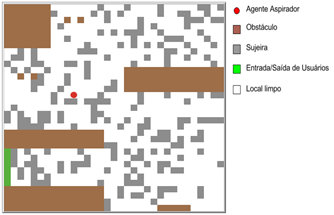
\includegraphics[width=10cm]{figuras/exp1-amb22}
    }{
        \Fonte{Elaborado pelo autor}
    }   
\end{figure}

O agente aspirador se movimenta pelo local visando limpar toda a sujeira nele contida. Ele deve evitar colisão com os obstáculos e procurar minimizar o gasto de energia. O ambiente é parcialmente observável e determinístico. As simulações das interações do sistema técnico com o ambiente consideram diversos cenários diferentes quanto à quantidade e distribuição inicial de sujeira, mas idênticos quanto à posição dos obstáculos no ambiente. 

\subsubsection{Modelo F}

A Figura \ref{fig:arq-agent-amb} ilustra a relação agente-ambiente, empregando o termo $AgentAmI$ para representar o programa de agente $AgSoftware$ componente do sistema técnico, cujo hardware é formado por um sensor e um atuador. A figura ilustra também outros termos empregados na concepção do quadro formal que define o modelo $F$. Em qualquer instante $k$ o sensor do aspirador percebe ($s^{*k}$) uma grade de $32 \times 32$ \textit{patches}, os quais podem ser do tipo limpo, sujo ou obstáculo, e o seu atuador executa uma ação adequada ($a^{*k}$) entre aquelas que são possíveis de serem executadas pelo aspirador.

\begin{figure}[h!]
    \centering
    \Caption{\label{fig:arq-agent-amb}– Interações do programa AgentAmi no ambiente Amb.} 
    \UECEfig{}{
        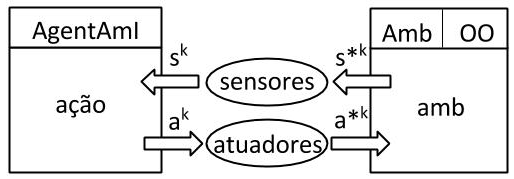
\includegraphics[width=6cm]{figuras/arq-agent-amb.png}
    }{
        \Fonte{Elaborado pelo autor}
    }   
\end{figure}

A figura identifica um episódio $Ep^K$ do programa $AgentAmI$ concebido para realizar o objetivo original $O_O$ no ambiente de tarefas $Amb$, tal que:

\begin{itemize}
    \item $S = \{s^1, s^2, \ldots \}$ -- Estados do ambiente –- em qualquer instante $k$ o sensor do aspirador disponibiliza um estado $s^k$ consistindo de uma grade menor, contida na grade $32\times32$ \textit{patches} que representa o local, de tamanho $3\times3$ \textit{patches}, ou seja, o conjunto de estados do ambiente é formado por todas as grades desse tamanho, em que cada \textit{patch} pode representar uma parte limpa (branco) ou suja (cinza) do local, ou a presença de um obstáculo (marrom) na parte;
    
    \item $A = \{a^1, a^2, \ldots \}$ -- Capacidade efetuadora -– em qualquer instante $k$ o atuador do aspirador consegue executar uma ação $a^k$ que pode ser: locomover-se do \textit{patch} em que o aspirador está para outro \textit{patch}, em qualquer direção (norte, sul, leste, oeste), ou limpar o \textit{patch} em que o aspirador está (aspirar);   
    
    \item ação:$S^*  \rightarrow A $ -- Comportamento -– função para seleção de ações em $A$ adequadas aos estados em $S$, ou seja, o aspirador deve aspirar em \textit{patches} cinza, e deve mudar para um \textit{patch} vizinho que seja cinza se estiver em um \textit{patch} branco;
    
    \item amb: $S\times A \rightarrow S$ -- Comportamento (determinístico) ambiente –- função para mudança de estados do ambiente de acordo com as ações executadas pelo agente – se o aspirador limpar em um \textit{patch} cinza então este deve mudar para branco, e se o aspirador seguir de um \textit{patch} para outro em uma determinada direção então mudar posição do agente para este outro \textit{patch}; 
    
    \item AgentAmI -- Um programa de agente implementando concretamente em linguagem NetLogo a função ação de um agente aspirador;
    
    \item Amb -- Um programa ambiente implementando concretamente em linguagem NetLogo a função amb;

    
    \item $\Omega$ -- Um conjunto formado por todas as grades de tamanho $32 \times 32$ \textit{patches}, diferentes quanto a quantidade de \textit{patches} do tipo cinza;
    
    \item $Cenario_i \in \Omega$ -- Uma grade de tamanho $32 \times 32$ \textit{patches}, os quais podem ser do tipo branco, cinza ou marrom; 
    
    \item $Cenario_i \in P(\Omega)$ -- Um subconjunto formado por $10 (N_{Cenarios})$ grades de $32 \times 32$ \textit{patches}, os quais podem ser do tipo branco, cinza ou marrom;
    
    \item $h(Cenario_i) \in (S\times A)^{Nint}$ -- Uma história formada por 100 ($NInt$) de $AgentAmI$ em $Amb$ correspondente ao $Cenario_i \in \Omega$; 
    
    \item $Ep^k(h(Cenario_i)) \in (S\times A)$ -- Um episódio na interação k, $k \leq 10$, da história de $AgentAmI$ em $Amb$ correspondente ao caso $Cenario_i \in \Omega$;
    
    \item $H(Cenario_i)) \in P((S\times A)^{Nint})$ -- Um conjunto de 10 histórias de comprimento 100 de $AgentAmI$ em $Amb$;
    
\end{itemize}

Neste experimento, o objetivo original ($O_O$) do sistema consiste em prestar um serviço de alta qualidade com um mínimo de despesas no ambiente. O modelo $F$ aplicado propõe definir formalmente $O_O$ por meio de uma função de utilidade, a qual considera um vetor de duas funções ($f_1$ e $f_2$) objetivos próximos ($O_1$ e $O_2$) de $O_O$, as quais têm o mesmo valor de importância no contexto de $O_O$, e são expressas em termos de duas funções escalares ($av_1$ e $av_2$), associadas aos atributos de descrição de estados, ou seja, a limpeza do ambiente e a quantidade de energia utilizada. A Tabela \ref{tab:objetivo-exp1} coloca em destaque os dois objetivos próximos e a notação empregada para as funções objetivos e escalares associadas.

\begin{table}[h!]   
    \centering
    \Caption{\label{tab:objetivo-exp1} Objetivos próximos do objetivo original.}
    \UECEtab{}{
        \begin{tabular}{cccc}
            \toprule
                Objetivo &  Descrição   &   Função Objetivo & Recompensa \\
                \midrule \midrule
                $O_1$  & Manter o ambiente limpo & $f_1(H(Cenarios))$ & $av_1(Ep^k(h(Cenario_i)))$ \\
                $O_2$  & Manter energia na bateria & $f_2(H(Cenarios))$ & $av_2(Ep^k(h(Cenario_i)))$ \\
            \bottomrule
        \end{tabular}
    }{
    \Fonte{Elaborado pelo autor}
}
\end{table}
    
Cada uma das funções escalares, $av_1$ e $av_2$, associa valores no domínio dos números reais, ou seja, valores de satisfação/insatisfação nos objetivos próximos $O_1$ e $O_2$, com um conjunto de episódios possíveis $(Ep(s,a) \in S\times A)$, descritos em termos de um conjunto de estados do ambiente ($s \in S$) e um conjunto de ações possíveis para o aspirador ($a \in A$). Abaixo a definição formal das funções escalares empregadas neste experimento:

\[
av_1(Ep((s^k, a^k)) =
\begin{cases}
  15 & \text{se $s^k$ = cinza e $a^k$ = aspirar,}\\
  0 & \text{se $s^k$ = branco e $a^k$ = aspirar,}\\
  0 & \text{se $s^k$ = cinza ou branco e $a^k$ = norte ou sul ou leste ou oeste}
\end{cases}
\]

e, 

\[
av_2(Ep((s^k, a^k)) =
\begin{cases}
  2 & \text{se $s^k$ = cinza ou branco e $a^k$ = aspirar,}\\
  1 & \text{se $s^k$ = cinza ou branco e $a^k$ = norte ou sul ou leste ou oeste}
\end{cases}
\]

Consequentemente, as funções objetivos podem ser definidas para para um conjunto formado por 10 cenários de teste ($N_{Cenarios}$ = 10), cada cenário associado a uma história formada por 100 episódios ($N_{Int}$ = 100) de interação do aspirador no ambiente:

\[
    f_1(H(\textrm{Cenários}))=\frac{1}{10}\sum_{i=1}^{10}Av_1(h(Cenario_i))
\]
e,
\[
    f_2(H(\textrm{Cenários}))=\frac{1}{10}\sum_{i=1}^{10}Av_2(h(Cenario_i)),
\]

tal que:

\[
Av_1(h(\textrm{Cenário}_i)) =  \sum_{k=1}^{100}av_1(Ep((s^k, a^k))
\]

e, 

\[
Av_2(h(\textrm{Cenário}_i)) = \sum_{k=1}^{100}av_2(Ep((s^k, a^k))
\]

E, finalmente, considerando-se que os dois objetivos próximos têm o mesmo valor de importância, a função utilidade para medir o alcance do objetivo original pelo aspirador pode ser definida.

\[ U(f(H(Cenarios)) = f_1(H(Cenarios)) - f_2(H(Cenario))\]

Assim, se o aspirador de pó for capaz de maximizar a função utilidade, isto é, se ele for capaz de maximizar a quantidade de patches limpos em 100 interações, minimizando o gasto de energia, então será adequado ao seu ambiente de tarefas, pois é capaz de realizar os objetivos próximos com os quais está comprometido e, consequentemente, de satisfazer o objetivo original do sistema.

\subsubsection{Modelo E}

O termo $AgentAmI$ na Figura \ref{fig:arq-agent-amb} foi empregado para representar o componente de software, ou seja, um programa de agente do tipo $AgSoftware$, do sistema técnico aspirador de pó, o qual tem como componentes de hardware um sensor e um atuador. Assim, de acordo com as propostas $P_2$ e $P_3$ na abordagem, este primeiro experimento considerou dois programas de agente do tipo $AgHardware$, um capaz de simular a realização do processamento de informações perceptivas ($s^{*k}$) realizado pelo sensor e outro para simular a execução de ações ($a^{*k}$) pelos atuadores do aspirador. A Figura \ref{fig:exp1-modelE} esboça os programas e a maneira como estão organizados na representação do sistema AmI.

\begin{figure}[h!]
    \centering
    \Caption{\label{fig:exp1-modelE}Organização de programas de agentes representando o robô aspirador.} 
    \UECEfig{}{
        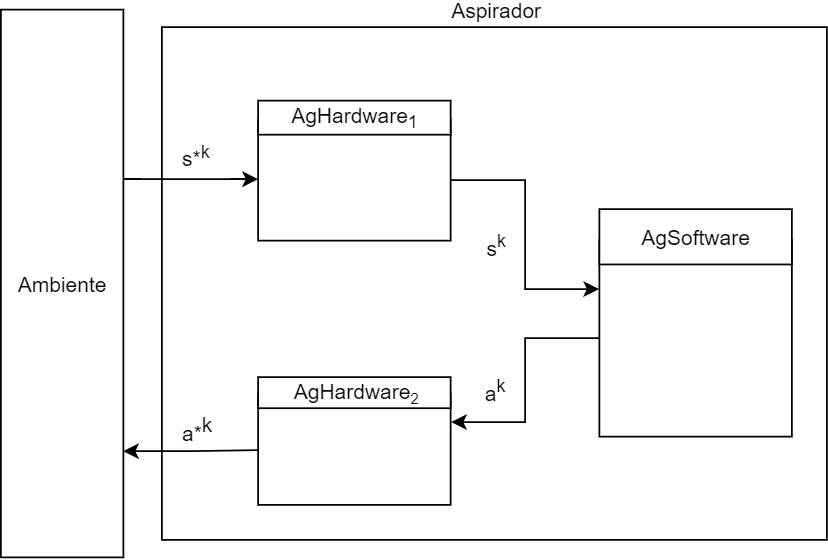
\includegraphics[width=6cm]{figuras/exp1-aspirador-modelE.png}
    }{
        \Fonte{Elaborado pelo autor}
    }   
\end{figure}

Os dois programas de agente $AgHardware_1$ e $AgHardware_2$ representam respectivamente o sensor e o atuador do sistema técnico no ambiente. O programa $AgSoftware$ processa as informações perceptivas oriundas do processamento do programa $AgHardware_1$, seleciona ações e envia para o programa $AgHardware2$, o qual deve executar estas ações no ambiente.

Quanto ao modelo $E$ associado à figura, consiste na definição dos conjuntos de programas de agentes e de papéis que os programas podem assumir na organização, das relações entre os papéis, dos grupos de programas e da cardinalidade destes grupos, ou seja: 

\begin{itemize}
    \item $Agents$ --	$\{AgHardware_1, AgHardware_2, AgSoftware\}$ – conjunto de três ($N_A = 3$) programas $AgentAmI$ na organização.
    
    \item $Roles$ -- $\{Device, Controller\}$ – conjunto de dois ($N_R = 2$) papéis que podem ser atribuídos aos programas de agentes $AgentAmI$.
    
    \item $AgentsRoles$ -- $\{AgentAmIDevice, AgentAmIController\}$ – família de dois ($N_R = 2$) conjuntos, tal que:
    
    \begin{itemize}
        \item $AgentAmIDevice$ -- $\{AgHardware_1, AgHardware_2\}$ – conjunto de programas no papel \textit{Device};
        \item $AgentAmIController$ -- $\{AgSoftware\}$ – conjunto de programas no papel \textit{Controller}.
    \end{itemize}
    
    \item $Bond$ -- \{$Bond_{knowledge}(AgentAmIDevice, AgentAmIController)$, 
                    \\$Bond_{knowledge}(AgentAmIController, AgentAmIDevice)$,
                    \\$Bond_{\textrm{Coordenação}}(AgentAmIDevice, AgentAmIController)$, 
                    \\$Bond_{\textrm{Coordenação}}(AgentAmIController, AgentAmIDevice)$\} – família de quatro relações entre os programas nos conjuntos $AgentAmIDevice$ e $AgentAmIController$, tal que:
    \begin{itemize}
        
        \item $Bond_{knowledge}(AgentAmIDevice, AgentAmIController)$ --	\{$(AgHardware_1, AgSoftware), \\(AgHardware_2, AgSoftware)$\} – programas $AgHardware_1$ e $AgHardware_2$ (papel \textit{Device}) têm o conhecimento da existência do programa $AgSoftware$ (papel \textit{Controller});
        
        \item $Bond_{knowledge}(AgentAmIController, AgentAmIDevice)$ -- \{$(AgSoftware$, $AgHardware_1$), ($AgSoftware$, $AgHardware_2$)\} – programa $AgSoftware$ tem o conhecimento da existência dos programas $AgHardware_1$ e $AgHardware_2$;
        
        \item $Bond_{\textrm{Coordenação}}(AgentAmIDevice, AgentAmIController)$ -- \{($AgHardware_1$, $AgSoftware$\} – cada ato de informação do programa $AgHardware_1$ ao programa AgSoftware gera o conhecimento correspondente no programa AgSoftware;
        
        \item $Bond_{\textrm{Coordenação}}(AgentAmIController, AgentAmIDevice)$ -- \{($AgSoftware$, $AgHardware_2$)\} – cada ato de informação do programa $AgSoftware$ ao programa $AgHardware_2$ gera o conhecimento correspondente no programa $AgHardware_2$
        .
    \end{itemize}
    
    \item $Groups$ --\{$AgHardware_1$, $AgHardware_2$, $AgSoftware$\} – família de um ($N_G = 1$) conjunto de programas de agentes exercendo seus papéis na organização.
    
    \item $Communication$ -- \{($AgHardware_1$, $AgSoftware$), ($AgSoftware$, $AgHardware_2$)\} – relação descrevendo quem pode enviar mensagens para quem na organização;
    
    \item $Frequency$ -- Figura \ref{fig:exp1-matriz-socio} – matriz sociométrica informa a frequência com que os programas de agentes trocam mensagens entre si.
    
\end{itemize}
    
    Os dois últimos itens descrevem a segunda parte do modelo. A Figura \ref{fig:exp1-matriz-socio} define a matriz sociométrica de acordo com o ponto de vista do projetista. Esta matriz permite ao projetista definir o mapa das interações que ocorrem entre os programas de agentes em diferentes papéis dentro dos grupos que compõem a organização. 
    
    \begin{figure}[h!]
        \centering
        \Caption{\label{fig:exp1-matriz-socio}Matriz sociométrica.} 
        \UECEfig{}{
            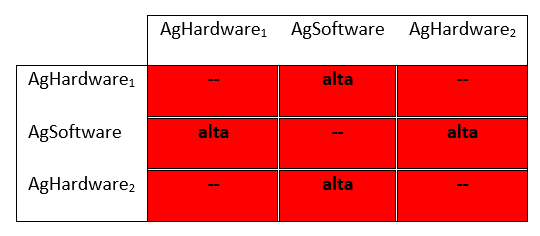
\includegraphics[width=6cm]{figuras/exp1-matriz-socio}
        }{
            \Fonte{Elaborado pelo autor}
        }       
    \end{figure}
    
    Por exemplo, A matriz sociométrica acima informa que a frequência \emph{freq($AgHardware_1$, \\AgSoftware)} com que o par de programas de agentes $(AgHardware_1, AgSoftware) \in Communication$ troca mensagens entre si é alta. A matriz informar estas concentrações de interações densas neste único grupo, de forma que as células com os maiores de valores de frequência ficaram ao longo da diagonal principal, e todos as células fora destes quadrados da diagonal têm valores de frequência zero.

\subsubsection{Modelo C}

O modelo comportamental descreve como a estrutura projetada deve funcionar para realizar o objetivo original do sistema, sua função descrita no modelo $F$, no ambiente de tarefas. O modelo de C neste primeiro experimento consiste na descrição formal dos procedimentos de tomada de decisão nos três programas de agentes em seus papéis na organização, $Agents = \{AgHardware_1, AgHardware_2, AgSoftware\}$, e dos processos que ocorrem dentro da organização, isto é, como os três programas de agentes integrados na estrutura organizacional devem agir.

No que diz respeito aos procedimentos de tomada de decisão, os “esqueletos” dos programas representando o agente aspirador de pó na Figura \ref{fig:exp1-modelE}, os programas $AgHardware_1$ e $AgHardware_2$, no papel $Device$ no modelo $E$, são do tipo reativo simples, e o programa $AgSoftware$, no papel $Controller$ no modelo $E$, também do tipo reativo. A Figura \ref{fig:exp1-modelC-detail} ilustra a customização dos esqueletos dos programas representando o agente artificial aspirador de pó único, interagindo com um ambiente que representa um local onde não existem pessoas transitando.

\begin{figure}[h!]
    \centering
    \Caption{\label{fig:exp1-modelC-detail}Esqueletos dos programas de agentes representando o sistema AmI.} 
    \UECEfig{}{
        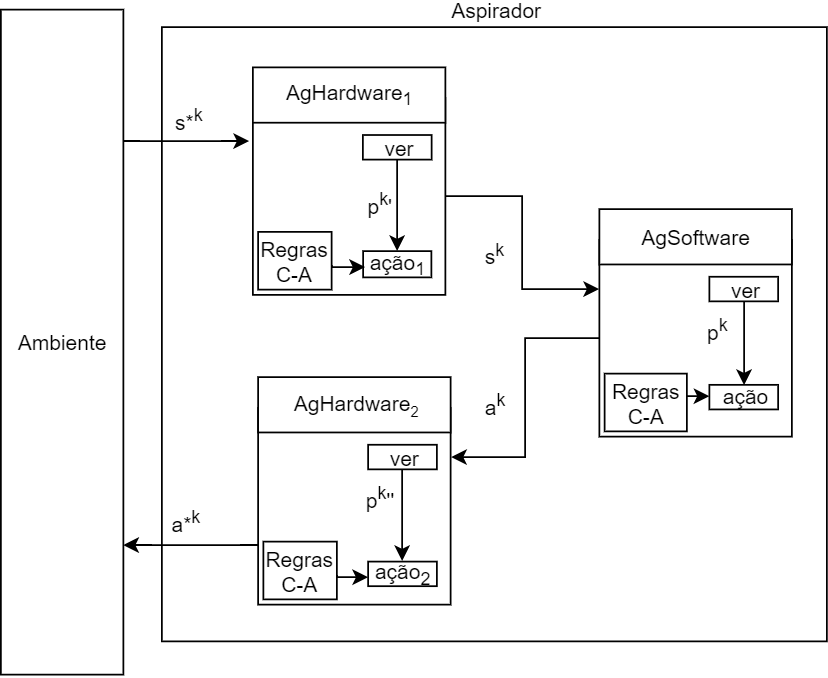
\includegraphics[width=10cm]{figuras/exp1-aspirador-G.png}
    }{
        \Fonte{Elaborado pelo autor}
    }   
\end{figure}

Estendendo-se o quadro desenvolvido no modelo $F$ para os três programas de agentes reativos, têm-se que:
\begin{itemize}
    \item $S^* = \{s^{*1}, s^{*2}, \ldots\}$ -- Estados do ambiente – em qualquer instante $k$ o programa $AgHardware_1$, representando o sensor do aspirador, percebe um estado $s^{*k}$ consistindo de uma grade de $32 \times 32$ \textit{patches} que representa uma parte do ambiente.
    
    \item $P_1 = \{p^{1\prime}, p^{2\prime}, \ldots \}$ -- Percepção do programa $AgHardware_1$ – 
    em qualquer instante $k$ o programa $AgHardware_1$ ao receber do ambiente entradas perceptivas $s^{*k} \in S^*$ – estados do 
    ambiente consistindo de uma grade de tamanho $32 \times 32$ 
    \textit{patches} – representa estas informações em uma linguagem interna adequada $p^{k\prime} \in P_1$.
    
    \item $ver_1: S^*  \rightarrow P_1$ --	Subsistema de percepção de $AgHardware_1$ – mapeia estados $s^{*k} \in S^*$ para percepções na linguagem interna $p^{k\prime} \in P_1$.
    
    \item $\textrm{ação}_1: P_1 \rightarrow S$ -- Subsistema de tomada de decisão de $AgHardware_1$ – função que mapeia percepções na linguagem $p^{k\prime} \in P_1$ em entradas perceptivas $s^k \in S$ – estados do ambiente consistindo de uma grade de tamanho $3 \times 3$ \textit{patches} – enviadas para o programa $AgSoftware$.
    
    \item $P = \{p^1, p^2, \ldots \}$ -- Percepção do programa $AgSoftware$ – em qualquer instante $k$ o programa $AgSoftware$ ao receber do programa $AgHardware_1$ as entradas perceptivas $s^k \in S$ – estados do ambiente consistindo de uma grade de tamanho $3 \times 3$ \textit{patches} – representa estas informações em uma linguagem interna adequada $p^k \in P$.
    
    \item $ver: S  \rightarrow P$ -- Subsistema de percepção de $AgSoftware$ – mapeia estados $s^k \in S$ para percepções na linguagem interna $p^k \in P$.
    
    \item $\textrm{ação}: P \rightarrow A$ -- Subsistema de tomada de decisão de $AgSoftware$ – função que mapeia percepções na linguagem $p^k \in P$ em descrições de ações $a^k \in A$ – locomover-se de um \textit{patch} para outro vizinho, em qualquer direção (norte, sul, leste, oeste), ou limpar o \textit{patch} em que o aspirador está (aspirar) – enviadas para o programa $AgHardware_2$.
    
    \item $P_2 = \{p^{1\prime\prime}, p^{2\prime\prime}, \ldots\}$	Percepção do programa $AgHardware_2$ – em qualquer instante $k$ o programa $AgHardware_2$ ao receber de $AgSoftware$ descrições de ações $a^k \in A$, representa estas informações em uma linguagem interna adequada $p^{k\prime\prime} \in P_2$.
    
    \item $ver_2: A  \rightarrow P_2$ -- Subsistema de percepção de $AgHardware_2$ – mapeia descrições de ações $a^k \in A$ para percepções em uma linguagem interna adequada $p^{k\prime\prime} \in P_2$.
    
    \item $\textrm{ação}_2: P_2 \rightarrow A$ -- Subsistema de tomada de decisão de $AgHardware_2$ – função que mapeia percepções na linguagem $p^{k\prime\prime} \in P_2$ em ações $a^{*k} \in A$ – locomover-se de um \textit{patch} para outro vizinho, em qualquer direção (norte, sul, leste, oeste), ou limpar o \textit{patch} em que o aspirador está (aspirar).
    
\end{itemize}

O conjunto de regras C-A do agente $AgHardware_1$ busca representar a noção de ambiente parcialmente observável pelo sensor do aspirador de pó, determinando a redução na quantidade de informações a respeito do ambiente presente em $p^{k\prime} \in P_1$, isto é, estados consistindo de uma grade de tamanho $32 \times 32$ \textit{patches} descritos na linguagem interna de $AgHardware_1$. Estas regras, orientam as ações deste programa, isto é, entradas perceptivas $s^k \in S$, neste experimento uma redução para uma grade de tamanho $3 \times 3$ \textit{patches}, enviadas para o programa $AgSoftware$. As regras C-A do $AgHarware_2$, neste momento, não interferem nas ações do agente  $Agsoftware$, ou seja, $a^{*k} = a^k \in A$.

O conjunto de regras C-A que orientam a seleção de ações adequadas à percepção $p^{k\prime\prime} \in P_2$, gerada na linguagem interna de $AgSoftware$ a partir das entradas perceptivas $s^k \in S$, geradas por $AgHardware_1$ e enviadas para o programa $AgHarware_2$, ou seja: locomover-se de um \textit{patch} para outro vizinho, em qualquer direção (norte, sul, leste, oeste), ou limpar o \textit{patch} em que o aspirador está. O algoritmo \ref{alg:exp1-behaviour} ilustra o conjunto de regras C-A incorporado no programa AgSoftware.

\begin{algorithm}[h!]
    %\SetSpacedAlgorithm
    \caption{\label{alg:exp1-behaviour} Conjunto de regras condição-ação do programa controlador AgSoftware.}
    %\Entrada{$p^k$ em S}
    %\Saida{$a^k$ em A}
    função ação ($p^k$ em S) retorna $a^k$ em A\\
    \Inicio{
        \ldots\\
        \textbf{se} $p^k$ (grade $3 \times 3$ \textit{patches}) \textit{patch} do aspirador cinza (sujo) \textbf{então} $a^k$ = aspirar\;
        \textbf{se} $p^k$ \textit{patch} do aspirador branco (limpo) e \textit{patch} cinza a norte  \textbf{então} $a^k$ = norte\;
        \textbf{se} $p^k$ \textit{patch} do aspirador branco e \textit{patch} cinza a sul  \textbf{então} $a^k$ = sul\;
        \textbf{se} $p^k$ \textit{patch} do aspirador branco e \textit{patch} cinza a leste  \textbf{então} $a^k$ = leste\;
        \textbf{se} $p^k$ \textit{patch} do aspirador branco e \textit{patch} cinza a oeste  \textbf{então} $a^k$ = oeste\;
        
        \textbf{se} $p^k$ \textit{patch} do aspirador branco e \textit{patch} marrom a norte  \textbf{então} $a^k$ = sul\;
        \textbf{se} $p^k$ \textit{patch} do aspirador branco e \textit{patch} marrom a sul  \textbf{então} $a^k$ = norte\;
        \textbf{se} $p^k$ \textit{patch} do aspirador branco e \textit{patch} marrom a leste  \textbf{então} $a^k$ = oeste\;
        \textbf{se} $p^k$ \textit{patch} do aspirador branco e \textit{patch} marrom a oeste  \textbf{então} $a^k$ = leste\;
        
        \textbf{se} $p^k$ \textit{patch} do aspirador branco e outros \textit{patches} brancos  \textbf{então} $a^k$ = mover-random\;
        
        \ldots\\
    }
\end{algorithm}

O conjunto de regras determina o comportamento do aspirador no ambiente de operação. Conforme indicado na seção que define o Modelo $F$, cada \textit{patch} possui uma cor simbolizando sujeira (ou não) e a presença de obstáculos. Em resumo, sempre que o aspirador estiver sobre um \textit{patch} de cor cinza ele deve selecionar a ação aspirar. Se ele estiver sobre um \textit{patch} branco (limpo) então deverá seguir para o local sujo mais próximo. Se o aspirador não detectar sujeira dentro do perímetro escaneado, ele escolherá de maneira aleatória uma direção para seguir em frente.

O conjunto de regras especificado visa exemplificar a descrição do componente de tomada de decisão do programa $AgSoftware$, por isso não foi detalhado com o rigor necessário para realizar os objetivos próximos do objetivo original, implícitos na função utilidade descrita no modelo $F$ da organização. O conjunto de regras encerra a especificação do modelo $C$ associado ao comportamento do componente de software do sistema \acrshort{ami} proposto no primeiro experimento.

Dando continuidade à descrição do modelo $C$, no que diz respeito à sua segunda parte, a Figura \ref{fig:exp1-protocol} descreve o protocolo de interação descrevendo as trocas de mensagens possíveis, no modelo $E$ descritas na relação Communication.

\begin{figure}[h!]
    \centering
    \Caption{\label{fig:exp1-protocol} Protocolo de interação entre os programas na organização.} 
    \UECEfig{}{
        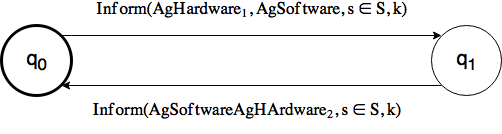
\includegraphics[width=8cm]{figuras/inform-protocol-hard-soft.png}
    }{
        \Fonte{Elaborado pelo autor}
    }   
\end{figure}

A relação $Communication$ descreve quem pode enviar mensagens para quem na organização, $Communication = \{(AgHardware_1, AgSoftware), (AgSoftware, AgHardware_2)\}$. A família de conjuntos de programas que compõem a organização, contém um único conjunto de três agentes, $G = \{{AgHardware_1, AgHardware_2, AgSoftware}\}$. O protocolo considera um conjunto de dois estados possíveis, $Q = \{q_0, q_1\}$. O estado inicial foi representado por $q_0$.

No início da interação, no instante $k$, o agente aspirador de pó percebe seu ambiente de tarefas por meio de seu sensor. Ou seja, o programa ambiente $Amb$ envia a informação $s^* \in S^*$ para o programa $AgHardware_1$, que, depois de processá-la, envia a informação $s \in S$ para o programa $AgSoftware$, isto é, $\delta(q_0, inform(AgHardware_1, AgSoftware, s \in S, k)) = q_1$. Posteriormente, o programa $AgSoftware$ processa essa informação, toma uma decisão e envia uma ação para ser executada no ambiente por um de seus atuadores. Ou seja, no modelo $C$, $AgSoftware$ envia a informação $a \in A$ para o programa $AgHardware_2$, $\delta(q_1, inform(AgHardware_2, AgSoftware, s \in S, k)) = q_0$, que, depois de processá-la, encerra a interação $k$ enviando uma ação $a^* \in A$ para o programa ambiente $Amb$.

Por motivos de simplicidade, a Figura \ref{fig:exp1-protocol} não ilustra as interações entre o aspirador e o seu ambiente de tarefas, isto é, o envio de mensagem contendo informação $s^* \in S^*$ do programa ambiente $Amb$ para o programa sensor $AgHardware_1$, e de mensagem contendo informação $a^* \in A$ do programa atuador $AgHardware_2$ para o programa $Amb$. A figura encerra a especificação do modelo \acrshort{fec} para o sistema \acrshort{ami} formado por um único aspirador em um local em que não existem pessoas transitando. A próxima subseção apresenta os objetos emergentes de interesse associados ao modelo $F$ deste sistema \acrshort{ami}. 

\subsubsection{Objetos Emergentes}

Conforme a Figura \ref{fig:sim-emergente-p6} indica. A simulação do sistema \acrshort{ami} utiliza como informações de entrada o modelo \acrshort{fec} construído para o sistema. Além disso, são utilizados dados do ambiente de tarefas e parâmetros de inicialização da aplicação, para descrever um contexto operacional de funcionamento do sistema no ambiente. Ao executar a simulação com as informações fornecidas, ela deve gerar como saída dados sobre o desempenho do sistema, conforme descrito no modelo $F$. Isto é, os objetos emergentes resultantes das interações descritas no modelo $C$, e da racionalidade das ações selecionadas pelos programas de agentes na organização estruturada no modelo $E$.

Este experimento buscou investigar o desempenho do programa $AgSoftware$, responsável pelo controle do agente artificial aspirador de pó, variando-se a quantidade inicial de sujeira no ambiente. Em um primeiro momento, o agente será inserido em um cenário onde 10\% dos \textit{patches} do ambiente estará sujo. Em cada um dos cenários posteriores a quantidade de \textit{patches} sujos será aumentada em 10\%. Serão ao todo dez cenários analisados, culminando em um cenário onde todos os \textit{patches} disponíveis estão sujos. 

Para cada um dos dez cenários de teste foram realizadas 100 simulações, totalizando mil execuções. A Figura \ref{fig:exp1-sim-exec} ilustra um exemplo da evolução dos valores das funções escalares empregadas neste experimento e da função utilidade, ao longo de 1000 interações do agente com o ambiente em um único cenário ambiental. 

\begin{figure}[h!]
    \centering
    \Caption{\label{fig:exp1-sim-exec} Medidas de desempenho em 1000 interações.} 
    \UECEfig{}{
        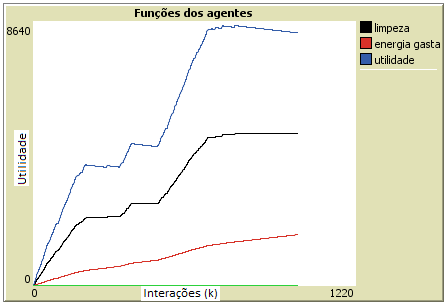
\includegraphics[width=8cm]{figuras/exp1-sim-exec.png}
    }{
        \Fonte{Elaborado pelo autor}
    }   
\end{figure}

A cada simulação executada são observadas informações a respeito dos objetivos próximos definidos no modelo $F$. Os objetivos $O_1$, manter o ambiente limpo, e $O_2$, economizar energia, são associados respectivamente as funções escalares $av_1$ e $av_2$. Essas funções são representadas na Figura \ref{fig:exp1-sim-exec} pelas curvas de limpeza e energia. A função Utilidade, que representa o desempenho do sistema em seu objetivo original $O_O$ (prestar um serviço de alta qualidade com um mínimo de despesas no ambiente), é composta por ambas as funções $av_1$ e $av_2$. Observando o comportamento dessas funções podemos deduzir informações sobre o desempenho do sistema \acrshort{ami}.

Uma coleção destas deduções, obtidas metodicamente pela execução de 100 simulações em cada cenário, permite a realização de inferências sobre o desempenho do sistema, em termos de medidas de distribuições, e se o mesmo será capaz de realizar o objetivo original em seu ambiente de tarefas. As Figuras \ref{fig:exp1-perf-limpeza} e \ref{fig:exp1-perf-utilidade} ilustram estas medidas de distribuições obtidas no primeiro experimento. 

\begin{figure}[h!]
    \centering
    \Caption{\label{fig:exp1-perf-limpeza} Distribuição do objetivo $O_1$.} 
    \UECEfig{}{
        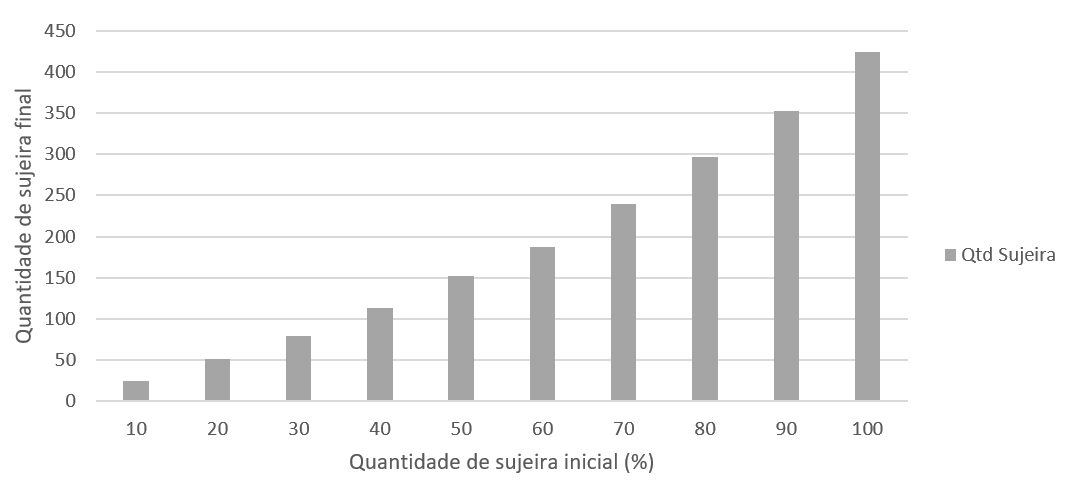
\includegraphics[width=10cm]{figuras/exp1-perf-limpeza.png}
    }{
        \Fonte{Elaborado pelo autor}
    }   
\end{figure}

A Figura \ref{fig:exp1-perf-limpeza} apresenta uma distribuição associada a quantidade de sujeira que permaneceu no ambiente ao fim da simulação. Representando a eficiência do agente em manter o ambiente limpo. Lembrando que medida associada ao objetivo $O_1$ representa a limpeza do ambiente da perspectiva do aspirador e não do ambiente. Não surpreendentemente, os resultados observados em cada um dos cenários caracterizam uma curva que cresce quase que linearmente à medida que aumenta a quantidade inicial de sujeira no ambiente.

\begin{figure}[h!]
    \centering
    \Caption{\label{fig:exp1-perf-utilidade} Distribuição de Utilidade do experimento.} 
    \UECEfig{}{
        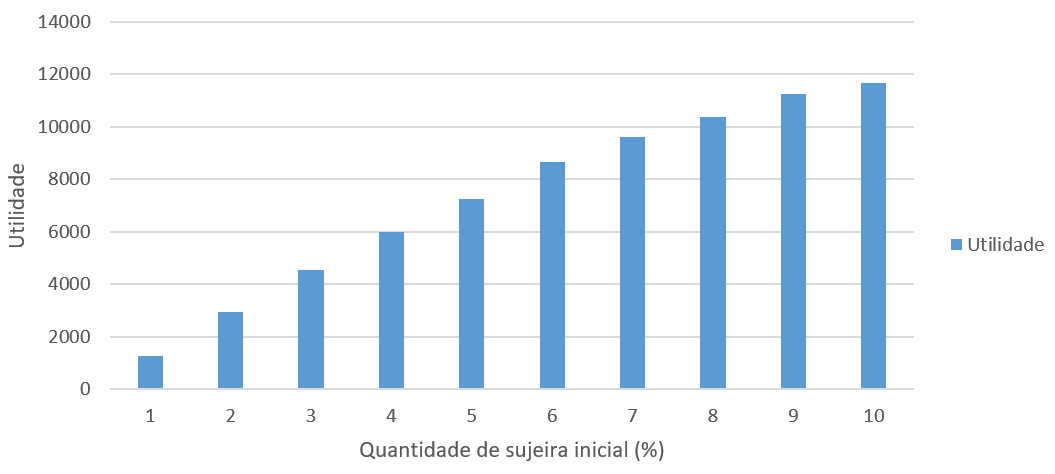
\includegraphics[width=10cm]{figuras/exp1-perf-utilidade.png}
    }{
        \Fonte{Elaborado pelo autor}
    }   
\end{figure}

Por outro lado, a distribuição associada à função utilidade, apresentada na Figura \ref{fig:exp1-perf-utilidade}, segue um padrão quase que logarítmico, tendendo a um valor máximo. Esse comportamento também já era esperado, pois, independente da estratégia de limpeza adotada, o sistema \acrshort{ami} é composto por um único agente aspirador para todo o ambiente. 


\subsection{Sistema AmI com um único sistema técnico em um ambiente não determinístico}
\label{sec:exp-dinamico}
Em vez de buscar melhorar o subsistema de tomada de decisão do programa controlador $AgSoftware$ no modelo $C$, nesta segunda parte do experimento vamos “injetar realidade” nas simulações envolvendo o mundo do aspirador de pó único, ou seja, tornando o ambiente dinâmico e não determinístico. Para simular um ambiente dinâmico, periodicamente o programa ambiente $Amb$ deposita sujeira em locais que foram previamente limpos pelo aspirador. Para simular um ambiente não determinístico o programa $AgHardware_2$, representando os atuadores do aspirador, poderá deixar de executar uma ação enviada por AgSoftware, caracterizando uma falha.

A simulação em um ambiente de tarefas não determinístico está relacionada com a proposta \textbf{P7} na abordagem. Especificamente neste experimento o projetista deve entender como os efeitos da aleatoriedade das ações executadas pelos atuadores do aspirador interferem na forma e nas propriedades macro de cada distribuição. Esse entendimento deve servir para garantir que este componente de confiabilidade baixa e integrado no aspirador, não o impedirá de alcançar o objetivo original em um ambiente de tarefas dinâmico. No que diz respeito ao modelo \acrshort{fec} associado ao experimento, somente o modelo $C$ deve ser alterado, mantendo-se os modelos $F$ e $E$ já definidos.

\subsubsection{Modelo C}

No que diz respeito aos procedimentos de tomada de decisão, os “esqueletos” dos programas $AgHardware_1$ e $AgSoftware$, são os mesmos apresentados na Figura \ref{fig:exp1-modelE}  e no resto do modelo $C$ descrito na mesma seção. Somente o esqueleto do programa $AgHadware_2$, no papel \textit{Device} no modelo $E$, deve sofrer alteração. No experimento anterior, as regras C-A do agente $AgHardware_2$ repetiam as ações que eram executadas pelo agente $AgSoftware$.

Neste experimento o programa $AgHardware_2$ será do mesmo tipo, porém, seu conjunto de regras será modificado para simular que os atuadores do aspirador estão sujeitos ao não determinismo. Ou seja, ele pode falhar em executar as ações selecionadas por $AgSoftware$. Mais formalmente em algumas ocasiões pode ser que $a^{*k} \neq a^k \in A$. 

O conjunto de regras C-A no subsistema de tomada de decisão de $AgHarware_2$ implementam as falhas possíveis no atuador do aspirador de pó, isto é, a ação $a^{*k} \in A$ que vai ser executada no ambiente, em função da ação $a^k \in A$ enviada por $AgSoftware$, mais especificamente, da representação desta informação $p^{k\prime\prime} \in P$, gerada na linguagem interna de $AgHardware_2$, e do instante $k$ das interações do aspirador com o seu ambiente. O algoritmo \ref{alg:exp2-behaviour} ilustra o conjunto de regras incorporado no programa $AgHardware_2$.


\begin{algorithm}[h!]
    %\SetSpacedAlgorithm
    \caption{\label{alg:exp2-behaviour} Conjunto de regras condição-ação do programa atuador $AgHardware_2$.}
    %\Entrada{$p^k$ em S}
    %\Saida{$a^k$ em A}
    função ação ($p^{k\prime\prime}$ em P) retorna $a^{*k}$ em A\\
    \Inicio{
        \ldots\\
        \textbf{se} $p^{k\prime\prime}$ = norte e falha(k) \textbf{então} $a^{*k}$ = move-random\;
        \textbf{senão se} $p^{k\prime\prime}$ = norte \textbf{então} $a^{*k}$ = norte\;
        \textbf{se} $p^{k\prime\prime}$ = sul e falha(k) \textbf{então} $a^{*k}$ = move-random\;
        \textbf{senão se} $p^{k\prime\prime}$ = sul \textbf{então} $a^{*k}$ = sul\;
        \textbf{se} $p^{k\prime\prime}$ = leste e falha(k) \textbf{então} $a^{*k}$ = move-random\;
        \textbf{senão se} $p^{k\prime\prime}$ = leste \textbf{então} $a^{*k}$ = leste\;
        \textbf{se} $p^{k\prime\prime}$ = oeste e falha(k) \textbf{então} $a^{*k}$ = move-random\;
        \textbf{senão se} $p^{k\prime\prime}$ = oeste \textbf{então} $a^{*k}$ = oeste\;

        \ldots\\
    }
\end{algorithm}

O conjunto de regras acima determina o comportamento do atuador do aspirador no ambiente de operação. Em resumo, $AgHarware_2$ pode não executar exatamente uma ação $a^k \in A$ enviada por $AgSoftware$. Dependendo do instante $k$, cada uma das ações pode falhar com uma certa probabilidade. Neste caso em que a função booleana falha(k) retorna um valor do tipo true, a ação $a^{*k} \in A$ executada por $AgHardware_2$ é igual à ação que retorna da função move-randon. Nos casos em que a função booleana falha(k) retorna um valor do tipo false, a ação $a^{*k}$ executada por $AgHardware_2$ é igual à ação selecionada por $AgSoftware$.

Nos experimentos, a probabilidade dos atuadores falharem aumenta à medida que o instante $k$ vai aumentando até chegar em 1000 interações, quando a simulação é terminada. O objetivo é simular algum tipo de desgaste que possa ocorrer com uso contínuo dos atuadores no mundo real. Apesar da possibilidade de não determinismo e do ambiente dinâmico nenhum refinamento ocorreu no esqueleto do programa $AgSoftware$ para lidar com estas mudanças nas propriedades do ambiente de tarefas. Entretanto, este refinamento pode ocorrer evoluindo o programa para o tipo orientado por metas ou, preferencialmente, orientado por utilidade. 

\subsubsection{Objetos Emergentes}

Os objetos emergentes analisados nesta subseção são extraídos de três experimentos distintos. O primeiro, e mais básico, é similar ao que já foi apresentado anteriormente. Nele vamos estudar novamente o comportamento do agente $AgSoftware$ em um ambiente estático, repetindo o primeiro experimento. No segundo vamos avaliar o comportamento desse mesmo agente, mas dessa vez ele estará inserido em um ambiente dinâmico, onde o programa do ambiente deposita novamente sujeira em locais que foram limpos previamente. Finalmente, no terceiro vamos utilizar o agente não determinístico nesse mesmo ambiente dinâmico. Nosso objetivo é comparar o desempenho do agente nessas três situações. As Figuras \ref{fig:exp2-perf-utilidade} e \ref{fig:exp2-perf-limpeza} ilustram as medidas de desempenho obtidas nesses experimentos.

\begin{figure}[h!]
    \centering
    \Caption{\label{fig:exp2-perf-utilidade} Distribuição de utilidade no experimento 2.} 
    \UECEfig{}{
        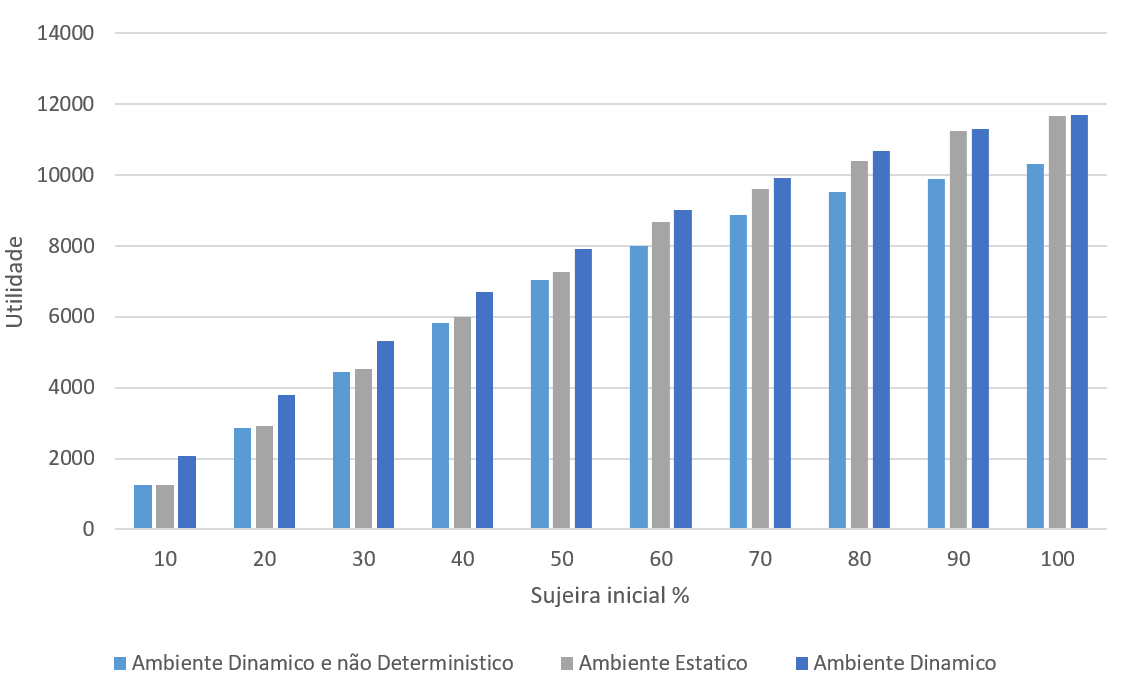
\includegraphics[width=10cm]{figuras/exp2-perf-utilidade.png}
    }{
        \Fonte{Elaborado pelo autor}
    }   
\end{figure}

Na Figura \ref{fig:exp2-perf-utilidade} acima podemos perceber que de todos os cenários observados, o que exibe um melhor desempenho é o cenário associado ao agente determinístico inserido em um ambiente dinâmico.  Isso acontece devido ao fato de a todo instante o ambiente depositar novas sujeiras em \textit{patches} limpos, aumentando o desempenho associado a função $av_1$ e, consequentemente, a utilidade.  O agente não determinístico possui o pior desempenho pois é o único com a desvantagem capaz de afetar a função $av_1$. 

\begin{figure}[h!]
    \centering
    \Caption{\label{fig:exp2-perf-limpeza} Distribuição do objetivo $O_1$ no experimento 2.} 
    \UECEfig{}{
        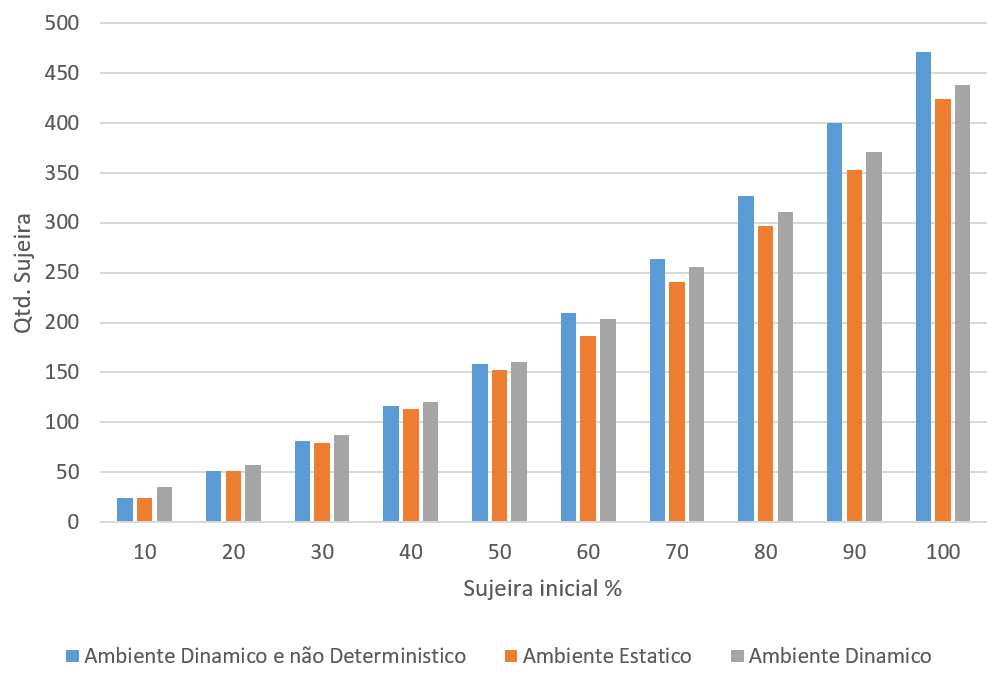
\includegraphics[width=10cm]{figuras/exp2-perf-limpeza.png}
    }{
        \Fonte{Elaborado pelo autor}
    }   
\end{figure}

As medidas associadas a quantidade de sujeira no fim do experimento deixam claro o quanto as falhas nos componentes do agente afetam em seu objetivo. Novamente o agente determinístico em ambiente estático teve um desempenho melhor, como era esperado. Mas o experimento em ambiente dinâmico, que também utiliza um agente determinístico, apresentou uma performance bastante similar. 

\subsection{Sistema AmI com um único sistema técnico em um ambiente com pessoas}
\label{sec:exp-user}
No experimento anterior observamos o comportamento do sistema operando com um único agente aspirador em um ambiente vazio e sem circulação de pessoas. No entanto, na aplicação real serão raras as ocasiões em que o agente estará sozinho no ambiente. Para tornar essa simulação um pouco mais condizente com realidade, neste experimento, vamos inserir no modelo do sistema um conjunto de agentes usuários que circulam pelo e ambiente e o modificam, interagindo com os aspiradores de forma indireta.

Cada agente usuário será representado por um único agente inteligente. Eles utilizam uma arquitetura reativa simples, e seu um único objetivo é sair do ambiente, mas sua principal função neste experimento é atrapalhar os agentes aspiradores. Na simulação, cada agente usuário é representado por um círculo azul, como ilustrado na Figura \ref{fig:exp2-5users}. 

\begin{figure}[h!]
    \centering
    \Caption{\label{fig:exp2-5users} Simulação do ambiente com cinco usuarios e um aspirador.} 
    \UECEfig{}{
        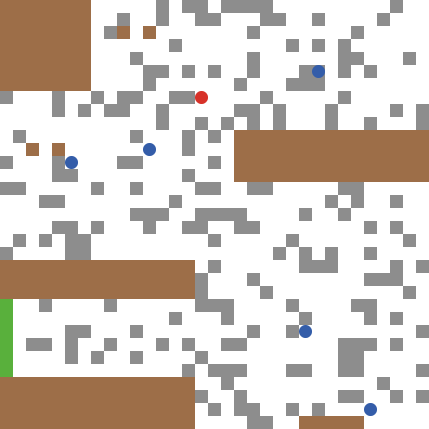
\includegraphics[width=6cm]{figuras/exp2-5users.png}
    }{
        \Fonte{Elaborado pelo autor}
    }   
\end{figure}

Este experimento será realizado no mesmo ambiente de simulação utilizado na seção \ref{sec:exp-dinamico}, ou seja, os agentes estarão inseridos em um ambiente dinâmico, que muda com o passar do tempo. Os aspiradores também deverão manter seus componentes não determinísticos que representam suas falhas. Dessa forma, os usuários serão inseridos em um ambiente dinâmico e não determinístico, mais próximo do que seria em um ambiente real. 

Conforme descrito na segunda seção do Capítulo \ref{cap:abordagem}, a proposta \textbf{P3} na abordagem consiste em uma descrição do sistema \acrshort{ami} por meio de uma organização de programas de agentes racionais, representando o software e o hardware componentes do sistema técnico, mas também as pessoas usuárias deste sistema. No que diz respeito ao modelo \acrshort{fec} da organização simulada nos experimentos anteriores, os modelos $F$, $E$ e $C$ neste experimento foram estendidos para acomodar as pessoas no sistema \acrshort{ami}. As subseções a seguir especificam o que foi estendido. 

\subsubsection{Modelo F}

Esta seção ilustra as alterações nos componentes do modelo $F$ da organização relacionados ao programa $AgSoftware$ no papel $Controller$ empregado nos dois experimentos anteriores. Apesar da presença de pessoas no ambiente, também representadas por programas de agentes na organização, a seção não dá ênfase às alterações nos componentes do modelo $F$ associados aos programas no papel de usuários, visto que os experimentos estão registrando o desempenho do programa no papel $Controller$. Entretanto, o mesmo tipo de especificação pode ser feito para os programas representando pessoas.

A Figura \ref{fig:arq-agent-amb} ilustra uma interação do sistema técnico ($AgentAmI$ = $AgSoftware$, hardware formado por um sensor e um atuador) com o ambiente em um instante $k$. Diferente do primeiro experimento, considerando que existem pessoas no ambiente, em qualquer instante $k$ o sensor do aspirador percebe ($s^{*k}$) uma grade de $32 \times 32$ \textit{patches}, os quais podem ser do tipo limpo, sujo, obstáculo ou pessoa. Assim, a primeira alteração no modelo $F$ está na descrição dos estados do ambiente do aspirador de pó:

\begin{itemize}
    \item $S = \{s^1, s^2, \ldots\}$ --	Estados do ambiente – em qualquer instante $k$ o agente $AgSoftware$ recebe o estado $s^k$ consistindo de uma grade de $3\times3$ \textit{patches}, contida no ambiente definido pelo cenário, que mostra as características dos \textit{patches} (branco, cinza e marrom) e quais agentes estão sobre eles (usuário e aspirador);
    
    \item $\textrm{ação} : S^*  \rightarrow A$ -- Comportamento – função para seleção de ações em $A$ adequadas aos estados em $S$, ou seja: o aspirador deve limpar \textit{patches} cinza, mudar para um \textit{patch} vizinho que seja cinza se estiver em um \textit{patch} branco, e deve mudar de direção se estiver em frente a um usuário;
    
\end{itemize}

A inserção de usuários no sistema permite que seja observada uma outra característica importante no seu desempenho. Para isso, devemos atualizar o objetivo original ($O_O$). Agora, além dos objetivos anteriores, manter o ambiente limpo e economizar energia, o agente aspirador deve também priorizar o bem estar dos usuários, evitando incomodá-los enquanto caminham pelo ambiente. Dessa forma, o objetivo original passa a ser composto por três vetores, ilustrados na tabela \ref{tab:objetivo-exp3}.

\begin{table}[h!]   
    \centering
    \Caption{\label{tab:objetivo-exp3} Objetivos próximos do terceiro experimento.}
    \UECEtab{}{
        \begin{tabular}{cccc}
            \toprule
                Objetivo &  Descrição   &   Função Objetivo & Recompensa \\
                \midrule \midrule
                $O_1$  & Manter o ambiente limpo & $f_1(H(Cenarios))$ & $av_1(Ep^k(h(Cenario_i)))$ \\
                $O_2$  & Manter energia na bateria & $f_2(H(Cenarios))$ & $av_2(Ep^k(h(Cenario_i)))$ \\
                $O_3$  & Evitar colisões com usuários & $f_3(H(Cenarios))$ & $av_3(Ep^k(h(Cenario_i)))$ \\
            \bottomrule
        \end{tabular}
    }{
    \Fonte{Elaborado pelo autor}
}
\end{table}

As funções escalares $av_1$ e $av_2$, definidas no experimento anterior não serão afetadas diretamente com a inserção dos agentes usuários. Mas agora precisamos definir uma função que associe o objetivo $O_3$ a um valor escalar, representando o desempenho do agente neste objetivo. A função $av_3$ é descrita em função do conjunto de episódios $Ep(s, a) \in S\times A$, onde $s \in S$ e $a \in A$. A definição dessa função é mostrada na equação abaixo. 

\[
Av_3(Ep((s^k, a^k)) =
\begin{cases}
  15 & \text{se $s^k$ = frente norte e azul e $a^k$ = norte,}\\
  15 & \text{se $s^k$ = frente sul e azul e $a^k$ = sul,}\\
  15 & \text{se $s^k$ = frente leste e azul e $a^k$ = leste,}\\
  15 & \text{se $s^k$ = frente oeste e azul e $a^k$ = oeste,}\\
  0 & \text{se $s^k$ = frente X e não azul e $a^k$ = Y,}\\
\end{cases}
\]
 tal que $X, Y \in \{ norte, sul, leste, oeste\}$ 

A função descrita acima associa os episódios em que o agente aspirador percebe usuários posicionados a sua frente e seleciona a ação de colidir. Essa ação representa a tentativa do agente aspirador de se mover em direção a um \textit{patch} já ocupado por um usuário. Dessa forma, em um conjunto formado por N cenários, onde cada cenários possui uma história de M episódios, temos que a função associada a $O_3$ é:

\begin{equation}
    f_3(H(Cenarios)) = \frac{1}{N}\sum_{k=1}^{N}Av_3(h(Cenario_i))
\end{equation}
, onde:
\begin{equation}
    Av_3(h(Cenario_i)) = \sum_{k=1}^{M}(Ep(s^k, a^k)
\end{equation}

Para finalizar o modelo F, a função utilidade do agente aspirador deve ser atualizada para medir os valores observados pela função $f_3$. Neste experimento consideramos que o objetivo $O_3$ tem um valor de importância maior que os outros objetivos. Portanto, a função utilidade do objetivo original do sistema será:
\begin{equation}
    Utilidade(f (H(Cenarios)))= f_1 (H(Cenarios)) + f_2 (H(Cenarios)) - 2 \times f_3 (H(Cenarios))
\end{equation}

Com essa atualização na função Utilidade, é possível observar o desempenho do sistema em situações onde o agente em um ambiente com usuários. Quanto mais usuários no ambiente, maiores serão as chances do aspirador se chocar com algum usuário, diminuindo o valor de utilidade e, portanto, seu desempenho. 

\subsubsection{Modelo E}

Como o usuário não faz parte do sistema técnico da aplicação, ele deve ser representado por um único agente. Isso significa que não existirão intermediários entre ele e o ambiente, logo suas percepções e ações dependem apenas de seus próprios sensores e atuadores. O programa de agente que interpreta o usuário na aplicação é chamado $AgUser$.

A definição da organização sistema elaborada no primeiro deve ser atualizada para que contemple também o agente usuário. Associando o programa de agente usuários aos seus respectivos papéis e ainda definindo suas relações com os outros agentes definidos previamente. 

\begin{itemize}
    \item Agents --	$\{AgHardware_1, AgHardware_2, AgSoftware, AgUser \}$ – conjunto de programas $AgentAmI$ na organização ($N_A = 4$).
    
    \item Roles	-- $\{Device, Controller, User\}$ – conjunto de papéis ($N_R = 3$) que podem ser atribuídos aos programas de agentes $AgentAmI$.
    
    \begin{itemize}
        \item $AgentAmIUser$ -- $\{AgUser_1, \ldots, AgUser_N\}$ – conjunto de programas no papel $User$;
    \end{itemize}
    
    \item $Bond_{knowledge}(AgentAmISoftware, AgentAmIUser)$ -- $\{$($AgSoftware$, $AgUser_1$), $\ldots$, ($AgSoftware$, $AgUser_M$)$\}$ – programa AgSoftware (papel $Controller$) têm o conhecimento da existência dos programas $AgUser_1, \ldots, AgUser_M$ (papel $User$), tal que $0 \leq M \leq N$;
    
    \item Groups -- \{$AgHardware_1$, $AgHardware_2$, $AgSoftware$, $AgPessoa_1$, $\ldots$, $AgPessoa_N$\} – família de um ($N_G = 1$) conjunto de programas de agentes exercendo seus papéis na organização.
\end{itemize}

As definições acima atualizam os conjuntos definidos nos experimentos anteriores. Os grupos omitidos não sofreram alterações. A última parte do modelo $E$ define os relacionamento de comunicação entre os agente. Porém, como o agente usuário não interage diretamente com nenhum agente do sistema técnico, não há necessidade de estabelecer um processo de comunicação entre eles. 

\subsubsection{Modelo C}

O modelo $C$ também deve ser atualizado neste experimento para descrever o comportamento do agente usuário e adequar o desempenho do agente aspirador aos novos estímulos. O agente usuário, por não precisar apresentar um comportamento complexo, é representado por um agente reativo simples, assim como os agentes $AgHardware_1$ e $AgHardware_2$ descritos no experimento anterior.  A Figura \ref{fig:exp3-modelC} abaixo mostra um esboço do agente usuário interagindo com o ambiente juntamente com os agentes definidos previamente.

\begin{figure}[h!]
    \centering
    \Caption{\label{fig:exp3-modelC} Esqueletos dos agentes definidos no terceiro experimento.} 
    \UECEfig{}{
        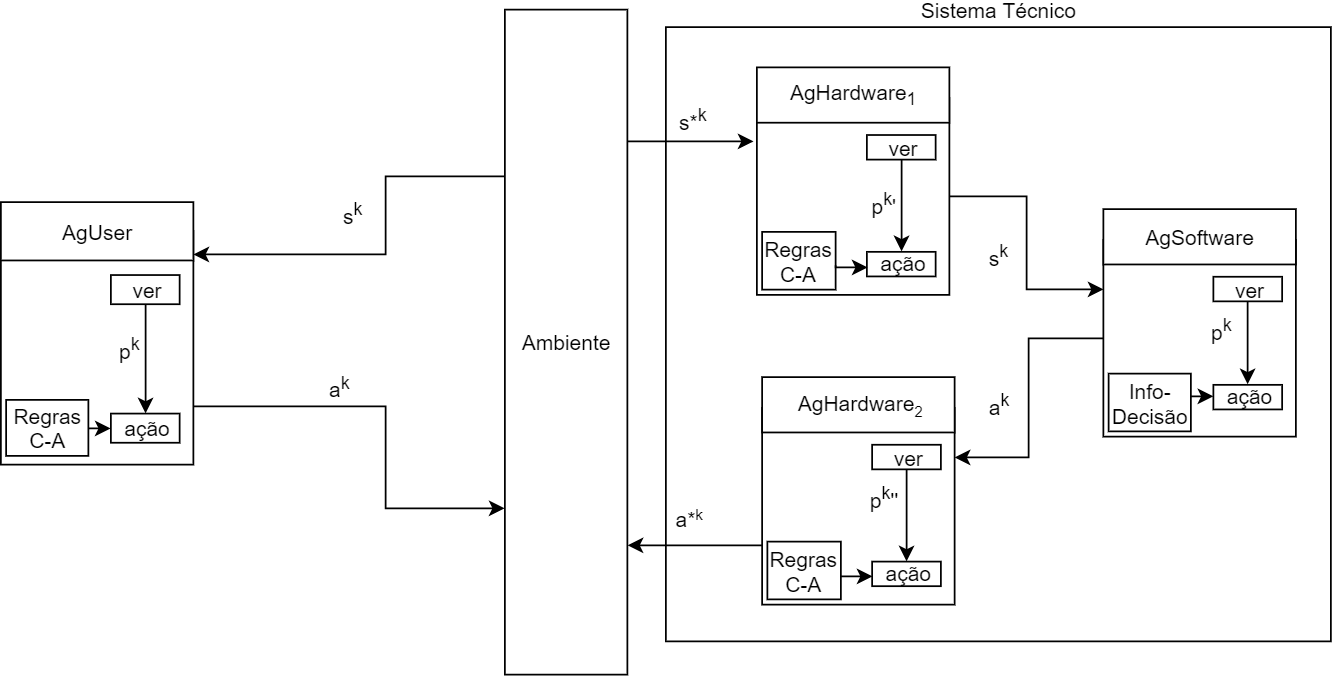
\includegraphics[width=10cm]{figuras/exp3-modelC.png}
    }{
        \Fonte{Elaborado pelo autor}
    }   
\end{figure}

O agente usuário enxerga o conjunto de estados do ambiente $s^k$ e utiliza sua função ver para extrair informação desse conjunto, formando sua percepção $p^k$. Utilizando suas regras C-A, o usuário informa ao ambiente qual foi a ação selecionada. O algoritmo \ref{alg:exp3-behaviour} abaixo apresenta o conjunto de regras condição-ação do agente usuário. 

\begin{algorithm}[h!]
    %\SetSpacedAlgorithm
    \caption{\label{alg:exp3-behaviour} Conjunto de regras condição-ação do programa $AgUser$.}
    %\Entrada{$p^k$ em S}
    %\Saida{$a^k$ em A}
    função ação ($p^{k\prime\prime}$ em P) retorna $a^{*k}$ em A\\
    \Inicio{
        \ldots\\
        \textbf{se} $p^{k}$ = cinza \textbf{então} $a^{*k}$ = move-random\;
        \textbf{se} $p^{k}$ = branco \textbf{então} $a^{*k}$ = throw-dirt\;
        \textbf{se} $p^{k}$ = verde \textbf{então} $a^{*k}$ = get-out\;
        \textbf{se} $p^{k}$ = marrom \textbf{então} $a^{*k}$ = change-dir\;
        \ldots\\
    }
\end{algorithm}

Sempre que o agente usuário fica sobre um \textit{patch} sujo, ele se move para um \textit{patch} vizinho aleatório. Se o usuário estiver sobre um \textit{patch} limpo a função \textit{throw-dirt} é acionada, fazendo com que o \textit{patch} se torne sujo com uma certa probabilidade. Nos experimentos realizados neste trabalho, a função \textit{throw-dirt} tem uma probabilidade de 5\% de sujar locais que o agente o usuário passa. A função \textit{get-out} é acionada sempre que o agente usuário encontrar a saída, representada por um conjunto de \textit{patches} verdes, quando executada o usuário sai do ambiente. 

Com relação ao aspirador, para que ele continue de acordo com o que foi definido no modelo $F$, é preciso atualizar suas regras condição-ação obedecendo aos objetivos adicionados. O objetivo próximo $O_3$, definido no modelo de função deste experimento, estabelece que o agente aspirador deve evitar incomodar os usuários prevenindo qualquer colisão com eles. Para isso, adicionamos a seguinte regra na base do agente AgSoftware:

\begin{algorithm}[h!]
    %\SetSpacedAlgorithm
    \caption{\label{alg:exp3-behaviour-asp} Nova regra do agente AgSoftware.}
    %\Entrada{$p^k$ em S}
    %\Saida{$a^k$ em A}
    função ação ($p^{k\prime\prime}$ em P) retorna $a^{*k}$ em A\\
    \Inicio{
        \ldots\\
        \textbf{se} user-close($p^{k}$) \textbf{então} $a^{*k}$ = move-away\;
        \ldots\\
    }
\end{algorithm}

A função \textit{user-close}, verifica o conjunto de percepções do agente aspirador buscando um agente usuário. Se for identificado que existe um usuário em uma posição dentro do raio de percepção do agente a função \textit{move-away} é acionada. Essa função usa a posição do usuário e a direção para a qual ele está apontando para determinar o caminho por onde ele deverá percorrer. Se a posição do aspirador estiver neste caminho, o aspirador deve girar noventa graus em relação ao usuário e se mover para o \textit{patch} vizinho.

Tendo em vista que os agentes usuários e os aspiradores não se comunicam diretamente, não é necessário alterar o comportamento de comunicação, definido anteriormente, para o agente aspirador. Na seção a seguir apresentamos os objetos emergentes obtidos na simulação criada a partir do modelo \acrshort{fec} apresentado. 

\subsubsection{Objetos Emergentes}

Diferente do experimento anterior, a quantidade inicial de sujeira no ambiente será mantida fixa em 25\% em todas as execuções. Nesta terceira prática, vamos observar o desempenho do agente AgSoftware no ambiente à medida que novos usuários são inseridos. Serão observados quinze cenários diferentes, no primeiro serão inseridos cinco usuários no ambiente de simulação, e a  cada cenário seguinte serão inseridos mais cinco, totalizando 75 usuários no ultimo experimento.

\begin{figure}[h!]
    \centering
    \Caption{\label{fig:exp3-sim-exec} Objetos emergentes em uma execução da simulação.} 
    \UECEfig{}{
        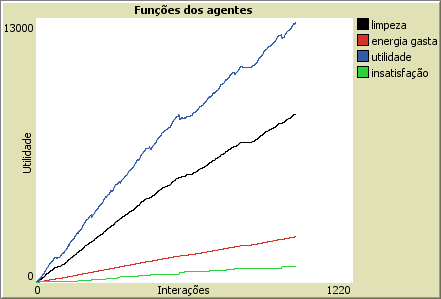
\includegraphics[width=8cm]{figuras/exp3-sim-exec.png}
    }{
        \Fonte{Elaborado pelo autor}
    }   
\end{figure}

A Figura \ref{fig:exp3-sim-exec} mostra as distribuições de cada um dos objetivos próximos do sistema durante a execução de um cenário que contem vinte usuários. A insatisfação, apresentada na cor verde, indica o desempenho do agente relacionado ao objetivo próximo $O_3$.  A Figura \ref{fig:exp3-perf-utilidade} abaixo apresenta um histograma da utilidade do aspirador durante os quinze cenários do experimento. 

\clearpage
\begin{figure}[h!]
    \centering
    \Caption{\label{fig:exp3-perf-utilidade} Utilidade do terceiro experimento.} 
    \UECEfig{}{
        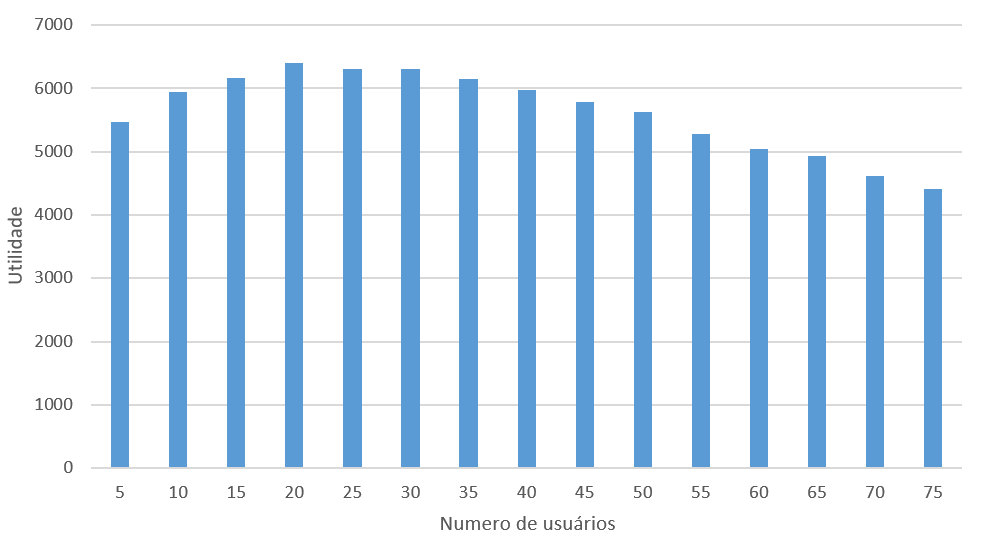
\includegraphics[width=10cm]{figuras/exp3-perf-utilidade.png}
    }{
        \Fonte{Elaborado pelo autor}
    }   
\end{figure}

Como podemos observar na Figura \ref{fig:exp3-perf-utilidade}, o valor da utilidade do agente aspirador, em um primeiro momento, cresce juntamente com o número de usuários no ambiente. Porém, do quinto cenário em diante esse valor passa a decrescer. Esse crescimento inicial é atribuído à propriedade do usuário de gerar novas sujeiras no ambiente, facilitando a busca do aspirador e consequentemente alimentando o objetivo próximo de manter o ambiente limpo ($O_1$). Mas a medida que o número de usuários cresce nos cenários seguintes, a utilidade passa a decrescer devido as penalidades impostas pelo novo objetivo próximo $O_3$, inserido nesse experimento. 

\begin{figure}[h!]
    \centering
    \Caption{\label{fig:exp3-perf-limpeza} Desempenho de limpeza no terceiro experimento.} 
    \UECEfig{}{
        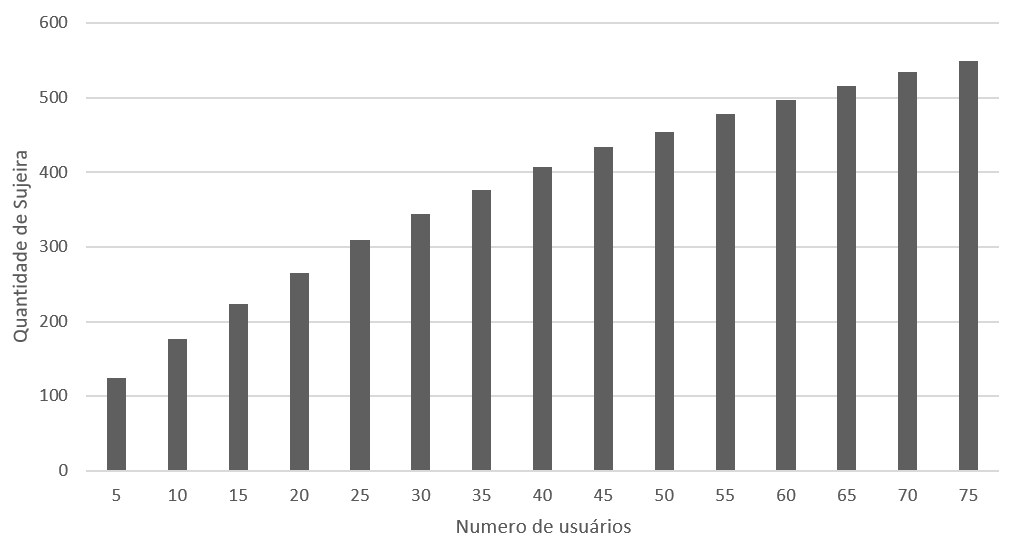
\includegraphics[width=10cm]{figuras/exp3-perf-limpeza.png}
    }{
        \Fonte{Elaborado pelo autor}
    }   
\end{figure}

A Figura \ref{fig:exp3-perf-limpeza} acima apresenta a variação de sujeira ao fim de cada um dos cenários.  É fácil perceber que quanto mais usuários no ambiente maior será a quantidade de sujeira inserida nele. Isso mostra que um único agente aspirador não é suficiente para manter o ambiente limpo quando grandes quantidades de pessoas circulam por ele.

\subsection{Sistema AmI com múltiplos aspiradores}
\label{sec:multi-asp}
No experimento anterior, inserimos um novo agente usuário, representando as pessoas que utilizarão o sistema \acrshort{ami}, em um ambiente dinâmico interagindo com um único agente aspirador não determinístico. Neste quarto experimento, vamos inserir outros aspiradores no ambiente e observar o desempenho do sistema em satisfazer seu objetivo original. 

O aspirador é representado por um conjunto de agentes que simulam o comportamento do aspirador de pó no ambiente. Cada aspirador é composto por dois agentes do tipo $AgHardware$ e um do tipo $AgSoftware$, como mostrado nos experimentos anteriores. As extensões inseridas no modelo \acrshort{fec} são explicadas a seguir.

\subsubsection{Modelo F}

Diferente do experimento anterior, que considera a existência de pessoas no ambiente, em qualquer instante $k$ o sensor do aspirador percebe ($s^{*k}$) uma grade de $32 \times 32$ \textit{patches}, os quais podem ser do tipo limpo, sujo, obstáculo, pessoa ou aspirador. Assim, a única alteração no modelo $F$ está na descrição dos estados do ambiente do aspirador de pó: 

\begin{itemize}
    \item $S = \{s^1, s^2, \ldots\}$ -- Estados do ambiente – em qualquer instante $k$ o sensor do aspirador disponibiliza um estado $s^k$ consistindo de uma grade menor, contida na grade $32 \times 32$ \textit{patches} que representa o local, de tamanho $3 \times 3$ \textit{patches}, ou seja, o conjunto de estados do ambiente é formado por todas as grades desse tamanho, em que cada \textit{patch} pode representar uma parte limpa (branco) ou suja (cinza) do local, ou a presença de um obstáculo (marrom), de uma pessoa (azul), ou de um aspirador (vermelho).
\end{itemize}

Apesar da presença de outros aspiradores, o objetivo original do sistema não foi modificado, mas é importante explicitar que outros objetivos poderiam ser adicionados. Poderíamos considerar como um outros objetivos próximos evitar colisões entre os próprios aspiradores, ou a cooperação entre eles. Porém, como o objetivo deste trabalho é apenas definir um modelo de criação de sistemas \acrshort{ami}, foi optado um caminho mais simples, mantendo os objetivos definidos anteriormente. 

\subsubsection{Modelo E}

A Figura \ref{fig:exp4-org-modelE} consiste em uma organização de programas de agentes racionais representando o sistema \acrshort{ami} formado por $M$ aspiradores de pó independentes. Cada programa $AgSoftware_i$ processa as informações perceptivas oriundas do processamento de seu programa $AgHardware_{1i}$, seleciona ações que evitem colisões com cada um dos $N$ programas representando pessoas, e envia estas ações para o seu programa $AgHardware_{2i}$, o qual as executa no ambiente.

\begin{figure}[h!]
    \centering
    \Caption{\label{fig:exp4-org-modelE} Organização de agentes no experimento quatro.} 
    \UECEfig{}{
        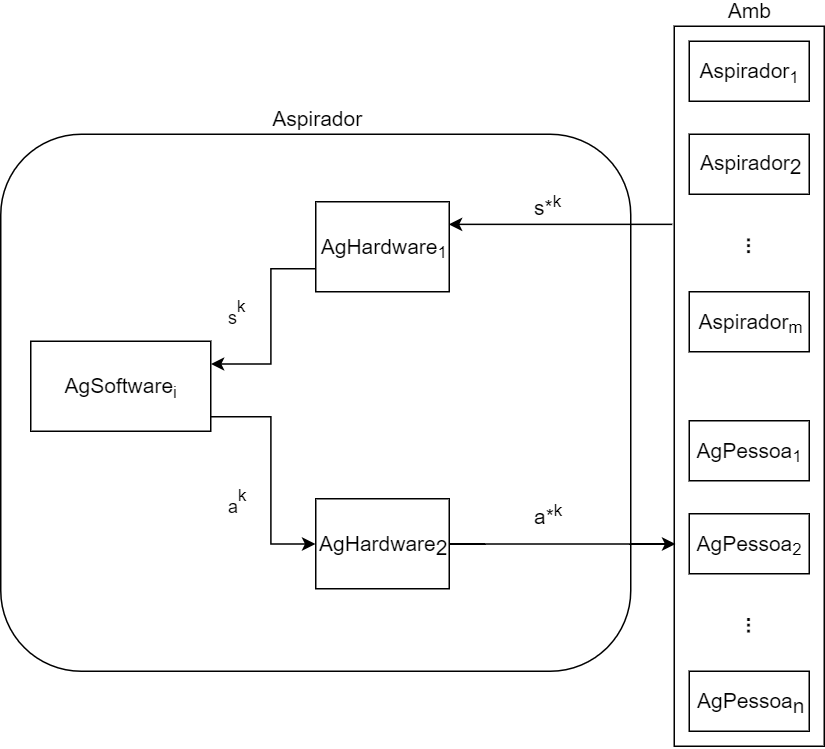
\includegraphics[width=8cm]{figuras/asp-exp4.png}
    }{
        \Fonte{Elaborado pelo autor}
    }   
\end{figure}

Quanto ao modelo E associado à figura, é necessário estender o conjunto de programas de agentes e de papéis que os programas podem assumir na organização, e de relações entre programas especificadas no último experimento, ou seja:

\begin{itemize}
    \item Agents -- \{$AgHardware_{11}$, $AgHardware_{21}$, $AgSoftware_1$, \ldots, $AgHardware_{1M}$, $AgHardware_{2M}$, $AgSoftware_M$, $AgPessoa_1$, \ldots, $AgPessoa_N$\} – conjunto $N_A = N + 3 \times M$ programas $AgentAmI$ na organização.
    
    \item AgentAmIDevice	\{$AgHardware_{11}$, $AgHardware_{21}$,  \ldots, $AgHardware_{1M}$, $AgHardware_{2M}$\} – conjunto de programas no papel \textit{Device};
    
    \item AgentAmIController	\{$AgSoftware_1$, \ldots, $AgSoftware_M$\} – conjunto de programas no papel \textit{Controller}.
    
    \item Bond	\{$Bond_{knowledge}$($AgentAmIDevice$, $AgentAmIController$),\\
            $Bond_{knowledge}$($AgentAmIControlle$r, $AgentAmIDevice$),\\
            $Bond_{\textrm{Coordenação}}$($AgentAmIDevice$, $AgentAmIController$),\\
            $Bond_{\textrm{Coordenação}}$($AgentAmIController$, $AgentAmIDevice$),\\
            $Bond_{knowledge}$($AgentAmIController$, $AgentAmIUser$),\\
            $Bond_{knowledge}$($AgentAmIController$, $AgentAmIController$)\} – família de seis relações entre os programas nos conjuntos $AgentAmIDevice$, $AgentAmIController$ e $AgentAmIUser$ tal que:
    
    \begin{itemize}
        \item $Bond_{knowledge}$($AgentAmIController$, $AgentAmIController$) --	\{($AgSoftware_1$, $AgSoftware_2$), \ldots , ($AgSoftware_1$, $AgSoftware_M$), \ldots, ($AgSoftware_M$, $AgSoftware_1$), \ldots, ($AgSoftware_M$, $AgSoftware_{M-1}$)\} – programa $AgSoftware_i$ (papel $Controller$) têm o conhecimento da existência dos programas $AgSoftware_1$, \ldots, $AgPessoa_N$ (papel $User$), tal que $0 \leq i \leq M$;
    \end{itemize}
    
    \item Groups -- \{$AgHardware_{11}$, $AgHardware_{21}$, $AgSoftware_1$, \ldots, $AgHardware_{1M}$, $AgHardware_{21}$, $AgSoftware_M$, $AgPessoa_1$, \ldots, $AgPessoa_N$\} – família de um ($N_G = 1$) conjunto de programas de agentes exercendo seus papéis na organização.
    
\end{itemize}

As informações apresentadas no modelo $E$ do último experimento que não são mencionadas no quadro acima não sofreram alterações com a adição  de outros aspiradores no ambiente. Apesar de cada programa $AgSoftware_i$ no papel $Controller$ poder conhecer um número $M-1$ de programas no papel $Controller$, não existe troca de mensagens entre eles. Dessa forma, a matriz sociométrica do primeiro experimento também não sofre alteração. 

\subsubsection{Modelo C}
Apesar dos aspiradores não trocarem mensagens entre si, o modelo comportamental descrito anteriormente foi estendido. O subsistema de tomada de decisão do programa AgSoftware sofreu alteração visando incorporar as percepções sobre os programas aspiradores (\textit{patches} em vermelho na simulação NetLogo), ou seja, pela presença de novas regras no conjunto. Mais especificamente, estas regras possibilitam que um aspirador evite colisões com outros aspiradores, mudando a direção de seu movimento sempre que perceber que está diante de outro aspirador no ambiente.

\subsubsection{Objetos Emergentes}

Para observar o comportamento do sistema neste experimento, analisamos três configurações do ambiente variando a quantidade de agentes aspiradores e de agentes usuários. Na primeira configuração fixamos a quantidade de aspiradores em três e variamos a quantidade de usuários da mesma forma que o experimento anterior. Na segunda dobramos a quantidade de agentes aspiradores, sendo seis agora.  E na terceira passam a circular no ambiente um total de doze agentes aspiradores. A Figura \ref{fig:exp4-perf-utilidade} abaixo mostra as distribuições obtidas observando a média da utilidade dos agentes. 

\begin{figure}[h!]
    \centering
    \Caption{\label{fig:exp4-perf-utilidade} Variação da utilidade no quarto experimento.} 
    \UECEfig{}{
        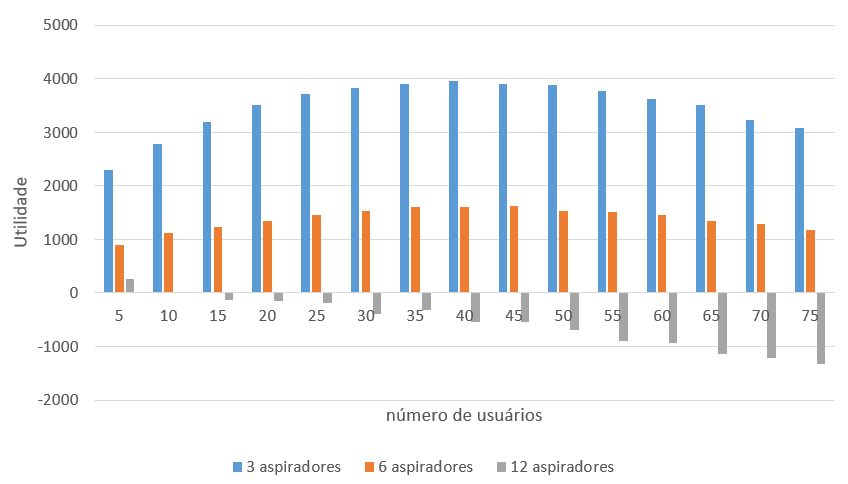
\includegraphics[width=10cm]{figuras/exp4-perf-utilidade.png}
    }{
        \Fonte{Elaborado pelo autor}
    }   
\end{figure}

Como o valor observado é a média das utilidades de cada um dos aspiradores, era esperado que os valores de utilidade decrescessem muito quando comparados aos experimentos anteriores. Um outro fator que também diminui a performance dos agentes neste experimento é quantidade de usuários. A medida que o número de pessoas no ambiente cresce a possibilidade dos aspiradores colidirem com eles também sobe, e como o peso associado ao objetivo próximo $O_3$ é maior que os outros, isso acaba causando uma grande queda nas medidas do $O_O$.

\begin{figure}[h!]
    \centering
    \Caption{\label{fig:exp4-perf-limpeza} Variação da limpeza no ambiente no quarto experimento.} 
    \UECEfig{}{
        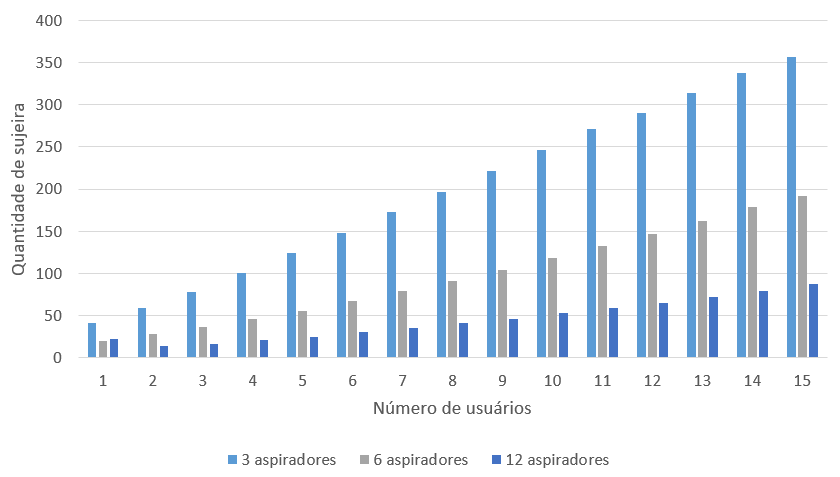
\includegraphics[width=10cm]{figuras/exp4-perf-limpeza.png}
    }{
        \Fonte{Elaborado pelo autor}
    }   
\end{figure}

Com relação a sujeira no ambiente, a Figura \ref{fig:exp4-perf-limpeza} acima deixa bem claro que a quantidade de aspiradores é uma propriedade muito importante para a limpeza do ambiente. Porém, como vimos na distribuição exibida pela Figura \ref{fig:exp4-perf-utilidade}, é necessário que exista uma mudança de estratégia para que o desempenho do sistema não seja afetado. 

\subsection{Sistema AmI com Agentes Coordenadores}
\label{sec:exp-coord}

No experimento anterior observamos o desempenho de um sistema \acrshort{ami}, composto por diversos agentes aspiradores, interagindo com múltiplos usuários em um ambiente. Apesar da grande quantidade de aspiradores apresentar bons resultados, em relação a limpeza do ambiente, sua utilidade tende a ser muito baixa. 

Esse desempenho é uma consequência direta do comportamento dos aspiradores. Apesar de existir um time de agentes que possuem o mesmo objetivo, não há nenhum tipo de cooperação entre eles. Cada um age como se estivesse sozinho, sem nenhuma comunicação com outros agentes. Além disso, a estratégia utilizada para buscar sujeira no ambiente obriga os aspiradores a se movimentarem continuamente, procurando por \textit{patches} sujos em áreas que já foram completamente limpas. 

Para tentar melhorar o desempenho do sistema, vamos adicionar uma nova entidade que estende o agente aspirador chamada de agente coordenador. Essa entidade será responsável por enviar mensagens a outros aspiradores, informando sobre locais com alta concentração de sujeira ou solicitando que o aspirador entre em modo de descanso.  Ele será representado na simulação por um círculo verde, como apresentado na Figura \ref{fig:exp5-agent-coord}.

\begin{figure}[h!]
    \centering
    \Caption{\label{fig:exp5-agent-coord} Agente coordenador no ambiente simulado.} 
    \UECEfig{}{
        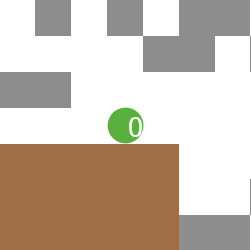
\includegraphics[width=4cm]{figuras/exp5-agent-coord.png}
    }{
        \Fonte{Elaborado pelo autor}
    }   
\end{figure}

Como o coordenador também é um tipo de aspirador, seu modelo de função não será alterado neste momento, porém é necessário alterar seus modelos de estrutura e comportamento. Nas subseções a seguir detalhamos adições necessárias nos modelos \acrshort{fec} para que este agente seja inserido na simulação.  

\subsubsection{Modelo E}

O agente coordenador também é composto por dois agentes do tipo AgHardware, representando seus sensores e atuadores e um do tipo AgSoftware, estruturados da de forma semelhante a apresentada na Figura \ref{fig:exp1-modelC-detail}. A seguir apresentamos as novidades na estrutura deste experimento. 

\begin{itemize}
    \item Agents -- \{$AgHardware_{11}$, $AgHardware_{21}$, $AgSoftware_1$, $AgHardware_{12}$, $AgHardware_{22}$, $AgSoftware_2$, $AgHardware_{13}$, $AgHardware_{23}$, $AgSoftware_3$, \ldots, $AgHardware_{1M}$, \\$AgHardware_{2M}$, $AgSoftware_M$, $AgPessoa_1$, \ldots, $AgPessoa_N$\} – conjunto com $N_A = N + 3 \times (3 + M)$ programas $AgentAmI$ na organização tal que $M \geq 0$, ou seja, existem pelos menos 3 aspiradores no local.

    \item Group --	\{$AgHardware_{11}$, $AgHardware_{21}$, $AgSoftware_1$, \ldots, $AgHardware_{1M}$, $AgHardware_{2M}$, $AgSoftware_M$, $AgPessoa_1$, ..., $AgPessoa_N$\} – família de conjuntos de programas de agentes ($N_G = 1$) exercendo seus papéis na organização.
    
    \item Bond -- \{$Bond_{Authority}(AgentAmIController, AgentAmIController)$\} – Relação de autoridade entre o agente controlador pertencente a um coordenador e um agente controlador pertencente a um aspirador.
    
    \begin{itemize}
        \item \{$Bond_{Authority}(AgentAmIController, AgentAmIController)$\} – \{($AgSoftware_1$, $AgSoftware_4$), ($AgSoftware_1$, $AgSoftware_5$), \ldots, ($AgSoftware_1$, $AgSoftware_M$), ($AgSoftware_2$, $AgSoftware_4$), ($AgSoftware_2$, $AgSoftware_5$), \ldots, ($AgSoftware_2$, $AgSoftware_M$), ($AgSoftware_3$, $AgSoftware_4$), ($AgSoftware_3$, $AgSoftware_5$), \ldots, ($AgSoftware_3$, $AgSoftware_M$)\} – cada  programa $AgSoftware_i$ (papel \textit{Controller}) pode delegar uma ou mais tarefas ao programa $AgSoftware_j$, onde i = \{1, 2, 3\}, e j = \{4, ..., M\};
    \end{itemize}

    \item Communication	-- \{$AgentAmIController$, $AgentAmIController$\} – relação descrevendo quem pode enviar mensagens para quem na organização;

\end{itemize}

O relacionamento de autoridade definido acima permite que um agente no papel \textit{Controller}, que faça parte de um coordenador, seja capaz de delegar tarefas a um outro agente no papel \textit{Controller} em um aspirador. Isso permite que os coordenadores enviem mensagens aos aspiradores contendo informações referentes a tarefas que eles irão executar. Neste experimento foram definidos três agentes, do tipo $AgSoftware$, que pertencem a entidade coordenador. Eles são representados na tabela de relacionamentos acima pelos agentes $AgSoftware_1$, $AgSoftware_2$ e $AgSoftware_3$.

\begin{figure}[h!]
    \centering
    \Caption{\label{fig:estrutura-coordenador} Relações do coordenador com outros agentes no ambiente.} 
    \UECEfig{}{
        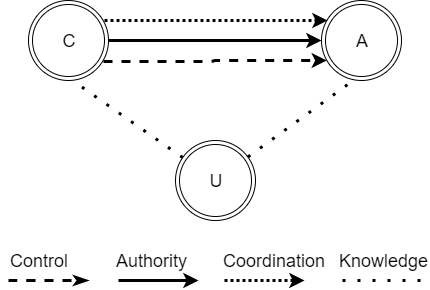
\includegraphics[width=6cm]{figuras/estrutura-coordenador.png}
    }{
        \Fonte{Elaborado pelo autor}
    }   
\end{figure}

A Figura \ref{fig:estrutura-coordenador} ilustra os relacionamentos entre as três entidades do experimento. Assim como o aspirador, o coordenador também tem um relacionamento \textit{knowledge} com o usuário. O que significa que seu relacionamento se limita ao conhecimento da existência um do outro. O relacionamento de autoridade entre o coordenador e o aspirador implica necessariamente na existência dos relacionamentos \textit{control}, \textit{coordination} e \textit{knowledge}.  Ou seja, além de delegar tarefas ao aspirador, este deve manter o coordenador informado sobre suas atividades.  A Figura \ref{fig:exp5-matriz-socio} apresenta a matriz sociométrica que relata a frequência de comunicação entre essas entidades. 

\begin{figure}[h!]
    \centering
    \Caption{\label{fig:exp5-matriz-socio} Matriz de relacionamento entre os agentes do quinto experimento.} 
    \UECEfig{}{
        \includegraphics[width=6cm]{figuras/exp5-matriz-socio}
    }{
        \Fonte{Elaborado pelo autor}
    }   
\end{figure}

Apesar de, internamente, os aspiradores e coordenadores serem uma composição de agentes do tipo $AgHardware$ e $AgSoftware$, podemos considerar que todos estão em um mesmo grupo na organização (vermelho). Esses novos relacionamentos inseridos no modelo de estrutura, ainda que simples, levam a grandes mudanças no comportamento dos agentes.  

\subsubsection{Modelo C}

Por ser uma extensão do aspirador, o coordenador também tem os mesmos objetivos definidos no objetivo original do sistema e, portanto, deve se comportar de forma a atingi-los. Mas por ser uma versão melhorada do aspirador, ele possui um conjunto de funções que o tornam mais complexo. A Figura \ref{fig:coordenador} mostra os esqueletos dos programas de agente que representam o coordenador. 

\begin{figure}[h!]
    \centering
    \Caption{\label{fig:coordenador} Esqueletos dos agentes que compõem o coordenador.} 
    \UECEfig{}{
        \includegraphics[width=10cm]{figuras/coordenador.png}
    }{
        \Fonte{Elaborado pelo autor}
    }   
\end{figure}

A maior diferença, apresentada na figura acima, entre o coordenador e o aspirador, é que o coordenador possui um AgSoftware do tipo orientado por objetivos. Isso permite que ele tenha um maior poder de decisão, além de possibilitar que sejam armazenadas informações sobre outras entidades do sistema. Abaixo apresentamos uma extensão do modelo F, definido no primeiro experimento, para o agente coordenador.

\begin{itemize}
    \item $P_1 = \{p^{1\prime\prime}, p^{2\prime\prime}, \ldots\}$ -- Percepção do programa $AgHardware_1$ – em qualquer instante $k$ o agente  $AgHardware_1$ ao receber do ambiente entradas perceptivas $s^{*k} \in S$ – estados do ambiente consistindo de uma grade de tamanho $5\times5$ \textit{patches}
    
    \item $\textrm{ação}_1: P_1 \rightarrow S$ -- Subsistema de tomada de decisão de $AgHardware_1$ – função que mapeia percepções $p^{k\prime\prime} \in P_1$ em entradas perceptivas $s^k \in S$ – estados do ambiente consistindo de uma grade de tamanho $5\times5$ \textit{patches} – enviadas para o programa $AgSoftware$.
    
    \item $P = \{p^1, p^2, \ldots\}$ -- Percepção do programa $AgSoftware$ – em qualquer instante $k$ o agente $AgSoftware$ ao receber do programa $AgHardware_1$ as entradas perceptivas $s^k \in S$ – estados do ambiente consistindo de uma grade de tamanho $5\times5$ \textit{patches} – representa estas informações em uma linguagem interna adequada $p^k \in P$.
    
    \item $\textrm{ação}: P \rightarrow A$	-- Subsistema de tomada de decisão de $AgSoftware$ – função que mapeia percepções na linguagem $p^k \in P$ em descrições de ações $a^k \in A$ – enviadas para o programa $AgHardware_2$.
    
\end{itemize}

O sensor do aspirador, definido no modelo de função do primeiro experimento, é capaz de perceber toda sujeira em um raio de três \textit{patches}, já o sensor do coordenador é capaz de sentir sujeira em um raio de até cinco \textit{patches}. Essa nova capacidade permite que o coordenador seja mais eficiente na busca por locais sujos. Ao encontrar sujeira, o coordenador pode enviar suas posições para outros agentes aspiradores no mesmo grupo, ou ir ao local e limpar ele mesmo. 

Além de informar aos aspiradores sobre a localização de sujeiras no ambiente, o coordenador também pode enviar uma série de mensagens para que os aspiradores possam agir de acordo com sua estratégia. Se o aspirador considerar que uma região do ambiente está limpa, ele pode emitir mensagens aos aspiradores próximos para que se movam ou para que entrem em modo de espera, evitando desperdiçar energia. 

\subsubsection{Objetos Emergentes}

As modificações no desempenho do sistema, com relação ao seu objetivo original podem ser observadas na Figura \ref{fig:exp5-perf-utilidade} abaixo.

\begin{figure}[h!]
    \centering
    \Caption{\label{fig:exp5-perf-utilidade} Utilidade do sistema no quinto experimento.} 
    \UECEfig{}{
        \includegraphics[width=12cm]{figuras/exp5-perf-utilidade}
    }{
        \Fonte{Elaborado pelo autor}
    }   
\end{figure}

A curva de utilidade observada para um primeiro cenário, onde temos apenas 3 agentes coordenadores no ambiente, é similar a curva apresentada no quarto experimento, onde tínhamos três aspiradores simultâneos no ambiente.  O desempenho passa a decrescer com a adição de novos agentes na simulação, porém, apresenta um ganho em relação ao experimento anterior.


\begin{figure}[h!]
    \centering
    \Caption{\label{fig:exp5-perf-limpeza} Limpeza do sistema no quinto experimento.} 
    \UECEfig{}{
        \includegraphics[width=12cm]{figuras/exp5-perf-limpeza}
    }{
        \Fonte{Elaborado pelo autor}
    }   
\end{figure}

Com relação a sujeira do ambiente, não é possível visualizar uma diferença significativa entre a abordagem utilizada no experimento anterior e a atual. Parte disso pode ser explicado pela nova estratégia utilizada, que permite ao coordenador enviar sinais de parada aos demais aspiradores, forçando eles a economizar energia mas impedindo que busquem por sujeira.


\subsection{Sistema Ami dividido em Grupos}
\label{sec:grupo}

Para tentar melhorar mais um pouco os valores de utilidade do sistema, neste experimento vamos modificar o modelo de estrutura da organização, dividindo os agentes em três grupos responsáveis por áreas diferentes do ambiente. O objetivo é espalhar melhor os aspiradores e os coordenadores, diminuindo sua necessidade de locomoção e maximizando sua área de cobertura. A Figura \ref{fig:exp6-ambiente} abaixo exemplifica como o ambiente será dividido. 

\begin{figure}[h!]
    \centering
    \Caption{\label{fig:exp6-ambiente} Divisão do ambiente no sexto experimento.} 
    \UECEfig{}{
        \includegraphics[width=6cm]{figuras/exp6-ambiente.png}
    }{
        \Fonte{Elaborado pelo autor}
    }   
\end{figure}

O ambiente da simulação será dividido em três zonas onde apenas os usuários são livres para circular entre elas. Cada zona terá um agente coordenador responsável, e cada aspirador atuará em uma dessas zonas. Tanto o coordenador quanto o aspirador podem circular apenas por suas zonas. 

Neste experimento, só foi necessário estender o modelo FEC da organização simulada nos experimentos anteriores nas suas dimensões estrutural (E) e comportamental (C), pois não surgiram novas entidades no ambiente, nem novos objetivos próximos. O modelo E foi alterado para acomodar o esquema de divisão em subgrupos. Já o modelo C foi alterado para acomodar os agentes coordenadores.

\subsubsection{Modelo E}

Para que o sistema seja capaz de se dividir no ambiente, conforme mostrado na Figura 54, é necessário estender o modelo de estrutura do conjunto de programas de agentes e de papéis que os programas podem assumir na organização, além das relações entre programas inseridas no último experimento. Mais especificamente, para o caso de três coordenadores conduzindo diferentes subgrupos de aspirador, alocados em zonas distintas do ambiente, onde cada subgrupo contém pelo menos o aspirador de pó coordenador, vale o seguinte modelo estrutural estendido:

\begin{itemize}
    \item Agents -- \{$AgHardware_{11}$, $AgHardware_{21}$, $AgSoftware_1$, $AgHardware_{12}$, $AgHardware_{22}$, $AgSoftware_2$, $AgHardware_{13}$, $AgHardware_{23}$, $AgSoftware_3$, \ldots, $AgHardware_{1M}$, \\$AgHardware_{2M}$, $AgSoftware_M$, $AgPessoa_1$, \ldots, $AgPessoa_N$\} – conjunto com $N_A = N + 3 \times (3 + M)$ programas $AgentAmI$ na organização tal que $M \geq 0$, ou seja, existem pelos menos 3 aspiradores no local, cada um em uma das três zonas e N pessoas espalhadas nas três zonas.

    \item Groups -- \{\{$AgHardware_{11}$, $AgHardware_{21}$, $AgSoftware_1$, \ldots, $AgHardware_{1Ma}$, 
    $AgHardware_{2Ma}$, $AgSoftware_{Ma}$, $AgPessoa_1$, \ldots, $AgPessoa_{Na}$\}, \{$AgHardware_{22}$, 
    $AgHardware_{22}$, $AgSoftware_2$, \ldots, $AgHardware_{1Mb}$, $AgHardware_{2Mb}$, $AgSoftware_{Mb}$, 
    $AgPessoa_1$, \ldots, $AgPessoa_{Nb}$\}, \{$AgHardware_{13}$, $AgHardware_{23}$, $AgSoftware_3$, \ldots, $AgHardware_{1Mc}$, $AgHardware_{2Mc}$, $AgSoftware_{Mc}$, $AgPessoa_1$, \ldots, $AgPessoa_{Nc}$\}\} – família de três ($N_G = 3$) conjuntos de programas de agentes exercendo seus papéis na organização, tal que $Ma + Mb +Mc = M$ e $Na + Nb +Nc = N$.
    
    \item Bond -- \{%$Bond_{knowledge}$($AgentAmIDevice$, $AgentAmIController$),\\
                % $Bond_{knowledge}$($AgentAmIController$, $AgentAmIDevice$), \\
                %$Bond_{\textrm{Coordenação}}$($AgentAmIDevice$, $AgentAmIController$),\\
                %$Bond_{\textrm{Coordenação}}$($AgentAmIController$, $AgentAmIDevice)$,   \\    
                %$Bond_{knowledge}$($AgentAmIController$, $AgentAmIUser$),\\
                %$Bond_{Autoridade$($AgentAmIController$, $AgentAmIController$),\\
                $Bond_{\textrm{Coordenação}}$($AgentAmIController$, $AgentAmIController$)\}
    – Relação de coordenação entre programas que utilizam do grupo $AgentAmIController$  tal que:
    \begin{itemize}
        \item $Bond_{\textrm{Coordenação}}$($AgentAmIController$, $AgentAmIController$) -- \{($AgSoftware_1$, $AgSoftware_2$), ($AgSoftware_1$, $AgSoftware_3$), \ldots, ($AgSoftware_1$, $AgSoftware_{Ma}$), ($AgSoftware_2$, $AgSoftware_1$), ($AgSoftware_2$, $AgSoftware_3$), \ldots ($AgSoftware_2$, $AgSoftware_{Mb}$), ($AgSoftware_3$, $AgSoftware_1$), ($AgSoftware_3$, $AgSoftware_2$), \ldots, ($AgSoftware_3$, $AgSoftware_{Mc}$)\} – cada ato de informação do programa $AgSoftware_i$ (papel \textit{Controller}) ao programa $AgSoftware_j$ ($i \neq j$) gera o conhecimento correspondente no programa $AgSoftware_j$;
    \end{itemize}

    \item Communication -- \{($AgSoftware_1$, $AgSoftware_2$), ($AgSoftware_1$, $AgSoftware_3$), \ldots, ($AgSoftware_1$, $AgSoftware_{Ma}$), ($AgSoftware_2$, $AgSoftware_1$), ($AgSoftware_2$, $AgSoftware_3$), \ldots ($AgSoftware_2$, $AgSoftware_{Mb}$), ($AgSoftware_3$, $AgSoftware_1$), ($AgSoftware_3$, $AgSoftware_2$), \ldots, ($AgSoftware_3$, $AgSoftware_{Mc}$)\}

\end{itemize}

Vale ressaltar que o modelo E anterior foi estendido a partir da inserção da relação $Bond_{\textrm{Coordenação}}$($AgentAmIController$, $AgentAmIController$) na família $Bond$ e de outros pares ordenados na relação $Communication$. Com esse novo relacionamento todos os agentes no papel $Controller$ passam a ser capazes de se comunicar, permitindo que exista uma maior cooperação entre eles. Ou seja, além da relação de autoridade entre os agentes no papel $Controller$ que compõem coordenadores e aspiradores, podemos contar também com a relação de coordenação entre os agentes $AgSoftware$ que compõem apenas os Coordenadores.

A matriz sociométrica descrita na Figura \ref{fig:exp6-matriz-socio}, define o mapa das interações que ocorrem entre os programas de agentes dentro de um mesmo subgrupo e entre os três programas coordenadores em subgrupos diferentes. 


\begin{figure}[h!]
    \centering
    \Caption{\label{fig:exp6-matriz-socio} Matriz sociométrica representando as interações entre os programas.} 
    \UECEfig{}{
        \includegraphics[width=\linewidth]{figuras/exp6-matriz-socio.png}
    }{
        \Fonte{Elaborado pelo autor}
    }   
\end{figure}

Na figura, a tabela menor indica que cada programa $AgAsp_i$ representa um aspirador $i$ do sistema técnico, ou seja, uma agregação de três programas na organização, isto é: $AgHardware_{1i}$, $AgHardware_{2i}$ e $AgSoftware_i$. A tabela maior informa uma baixa frequência de troca de mensagens entre os três coordenadores ($AgAsp_1$, $AgAsp_2$, $AgAsp3$) dos três grupos, uma frequência média entre os coordenadores de cada grupo e os seus coordenados ($AgAsp_1$, \ldots, $AgAsp_{Ma}$; $AgAsp_2$,  \ldots, $AgAsp_{Mb}$; $AgAsp_3$, \ldots, $AgAsp_{Mc}$), e que tanto coordenadores quanto seus coordenados não interagem com os programas representando as pessoas nas três zonas ($AgPessoa_1$, \ldots, $AgPessoa_{Na}$; $AgPessoa{Na+1}$, \ldots, $AgPessoa_{Nb}$; $AgPessoa_{Nb+1}$, \ldots, $AgPessoa_{Nc}$).

\subsubsection{Modelo C}

Conforme mencionado, o modelo $C$ foi alterado para acomodar os agentes coordenadores. Esta acomodação implicou na definição do comportamento de cada programa no papel $Controller$ coordenando um dos três grupos ($AgSoftware_1$, $AgSoftware_2$, $AgSoftware_3$), em uma alteração no modelo do comportamento dos outros programas no papel $Controller$ coordenados em um dos grupos ($AgSoftware_4$, \ldots, $AgSoftware_{Na}$, $AgSoftware_{Na+1}$, \ldots, $AgSoftware_{Nb}$, $AgSoftware_{Nb+1}$, \ldots, $AgSoftware_{Nc}$), e no protocolo de interação entre os programas.

Apesar do modelo $F$ não ter sido estendido, as informações sobre os estados do ambiente, percebidas pelos programas no papel \textit{Device} representando sensores, agregam informações a respeito de linhas divisórias entre as zonas compondo o ambiente. Assim, quando recebem estas informações, os programas no papel \textit{Controller} sendo coordenados e coordenadores evitam ultrapassar estas linhas. Entretanto, sempre que precisar, um coordenador pode requisitar a outro coordenador que envie alguns dos aspiradores para a sua zona. Neste caso o coordenador que recebeu a mensagem deve consultar seus coordenados visando descobrir aspiradores disponíveis, os quais devem assimilar a ideia e partir para a zona que requisitou ajuda. 

A Figura \ref{fig:exp6-protocolo} ilustra o protocolo de interação entre os programas no papel \textit{Controller}. A descrição do processo de comunicação considera um conjunto de seis estados possíveis, $Q = \{q_0, q_1, q_2, q_3, q_4, q_5\}$, em que o estado inicial foi representado por $q_0$. A figura supõe que o processo de conversação envolve um uma família de quatro conjuntos de programas $G = \{C, C_1, C_2, C_3\}$, ou seja: um conjunto de três programas coordenadores $C = \{AgAsp_1, AgAsp_2, AgAsp_3\}$, um conjunto de programas coordenados pelo coordenador $AgAsp_1$ da zona 1, isto é, $C_1 = \{AgAsp_4, \ldots, AgAsp_{Ma}\}$; um conjunto de programas coordenados pelo coordenador $AgAsp_2$ da zona 2, isto é, $C_2 = \{AgAsp_{Ma+1}, \ldots, AgAsp_{Mb}\}$; e um conjunto de programas coordenados pelo coordenador $AgAsp_3$ da zona 3, isto é, $C_3 = \{AgAsp_{Mb+1},  \ldots, AgAsp_{Mc}\}$.

\begin{figure}[h!]
    \centering
    \Caption{\label{fig:exp6-protocolo} Protocolo de interação entre os programas na organização.} 
    \UECEfig{}{
        \includegraphics[width=10cm]{figuras/exp6-protocolo.png}
    }{
        \Fonte{Elaborado pelo autor}
    }   
\end{figure}

De acordo com a relação Communication, o protocolo de interação indica que os programas coordenadores se comunicam entre si e cada um com os programas por ele coordenados. As transições entre os estados $q_0-q_1$ e $q_4-q_5$ correspondem a solicitações envolvendo pelo menos três agentes (\textit{requests to request}), a transição entre os estados $q_1-q_2$ corresponde a uma pergunta (\textit{requests to inform}) envolvendo pelo menos dois agentes. O restante das transições corresponde às mensagens fundamentais para solicitar e informar (\textit{request e inform}) a um outro agente.

No instante $t_1$, a partir do estado inicial $q_0$, existem duas possibilidades de transição. Primeiro, qualquer coordenador $s$ no conjunto de coordenadores $C$ pode solicitar que cada coordenador $h_i$ no conjunto $C$ solicite que seus coordenados no conjunto $C_i$ se dirijam à zona do coordenador $s$. No instante $t_2$ o coordenador $h_i$ em C pergunta aos seus coordenados em $C_i$ a respeito de seus estados atuais. No instante $t_3$ um programa $h$ em $C_i$ que está livre, informa este fato ao seu coordenador $h_i$ em $C$. No instante $t_4$ o coordenador $h_i$ solicita que seu coordenado $h$ se dirija à zona do coordenador $s$, o qual solicitou esta ação no instante $t_1$.

Na segunda transição possível no instante $t_1$, um programa coordenado $h$ em um conjunto $C_i$ informa ao seu coordenador $h_i$ em $C$ que está livre. Sendo assim, se em $t_2$ algum coordenador $s$ em $C$ solicitar que o coordenador $h_i$ solicite que seus coordenados se dirijam à zona do coordenador $s$, então em $t_3$ o coordenador $h_i$ poderá solicitar imediatamente que $h$ no conjunto $C_i$ se dirija a zona de $s$, o qual solicitou esta ação no instante $t_2$, depois que $h$ informou que estava livre em $t_1$. 

A Figura \ref{fig:exp6-protocolo} omitiu a transição para o estão inicial $q_0$ na situação em que os programas coordenados e/ou coordenadores não enviam mensagens de retorno para as solicitações. Por exemplo, depois de $\epsilon$ unidades de tempo, contadas a partir do horário de início da conversação no instante $t_2 (time(t_2))$ até um tempo limite em que uma mensagem de retorno deve ser enviada no instante $t_3 (time(t_3))$, o protocolo deve transitar para o estado inicial, $\delta(q_2, time(t_3) – time(t_2) > \epsilon) = q_0$, em que os programas poderão iniciar novo processo de conversação.

\subsubsection{Objetos Emergentes}

Os objetos emergentes, resultantes das modificações realizadas neste experimento, são apresentados nesta subseção. As condições são as mesmas observadas no experimento anterior. Em cada teste serão três coordenadores, cada um responsável por uma zona. A quantidade de aspiradores por teste será variada da mesma forma que o experimento anterior. 

\begin{figure}[h!]
    \centering
    \Caption{\label{fig:exp6-perf-utilidade} Utilidade do sistema ni sexto experimento.} 
    \UECEfig{}{
        \includegraphics[width=10cm]{figuras/exp6-perf-utilidade}
    }{
        \Fonte{Elaborado pelo autor}
    }   
\end{figure}

Conforme podemos observar na Figura \ref{fig:exp6-perf-utilidade}, o desempenho do sistema foi bem inferior aos experimentos anteriores. Isso pode ser atribuído a um fator observado durante a execução. Como tanto os coordenadores quanto os aspiradores tem um espaço de movimento mais limitado, quando eles se posicionam em certas áreas, como nos cantos de suas respectivas zonas, eles tem menos opções de movimento, forçando o agente a seguir por uma direção que pode estar ocupada por algum usuário causando uma colisão com ele.  Como a função associada ao objetivo de evitar incomodar os usuários tem prioridade maior que as outras, o desempenho do sistema é bastante afetado. 

\begin{figure}[h!]
    \centering
    \Caption{\label{fig:exp6-perf-limpeza} Limpeza do ambiente no sexto experimento.} 
    \UECEfig{}{
        \includegraphics[width=10cm]{figuras/exp6-perf-limpeza}
    }{
        \Fonte{Elaborado pelo autor}
    }   
\end{figure}

Como podemos observar na Figura \ref{fig:exp6-perf-limpeza} acima, não é possível determinar uma diferença significativa entre o desempenho, relacionado a limpeza do ambiente, neste experimento e no observado na Figura \ref{fig:exp5-perf-limpeza}. Isso reforça a hipótese que a baixa performance do objetivo original está relacionada ao objetivo próximo $O_3$.

\section{Conclusão}
\label{sec:conclusao}

Neste capítulo foi mostrada a utilização do modelo \acrshort{fec}, elaborado no capítulo \ref{cap:abordagem}, para uma aplicação de sistemas de inteligência ambiental. Para construir o modelo dessa aplicação foi utilizada uma abordagem incremental, inserindo novos elementos no sistema a cada experimento e, consequentemente, aumentando sua complexidade. Cada um dos experimentos gera um conjunto de dados que são utilizados para avaliar o modelo construído para o sistema. 
A aplicação utilizada para o teste desse modelo tem como base o experimento clássico do aspirador de pó. Ela consiste em um sistema de inteligência ambiental onde um conjunto de agentes aspiradores de pó deve manter limpo um ambiente onde circulam grupos de pessoas. O objetivo desse sistema \acrshort{ami} é manter o ambiente limpo, minimizando os custos de energia e evitando atrapalhar as pessoas que estão passando.

No primeiro experimento realizado, a aplicação é simulada em um ambiente estático contendo apenas um agente aspirador. O intuito deste experimento é verificar se o modelo gerado para o agente aspirador é capaz de cumprir um dos objetivos da aplicação, limpar o ambiente, e validar o modelo de função gerado para esse objetivo. 

O segundo experimento também tem como objetivo observar o comportamento do agente e de seu modelo de função, mas dessa vez em um condições diferentes. O agente aspirador único é mantido na aplicação, porém, o ambiente de aplicação se torna dinâmico. Ou seja, o próprio programa de ambiente passa a inserir sujeira no ambiente. Além disso, o agente aspirador passa a apresentar falhas em seu atuador, perdendo sua característica determinística.

O terceiro experimento mantém as novas características do ambiente e do agente aspirador, e adiciona um novo elemento a simulação, o agente usuário. Neste experimento são observadas as medidas extraídas, a partir do modelo de função atualizado, da simulação em função da quantidade de pessoas no ambiente.

No quarto experimento passamos observar na simulação um ambiente contendo dois ou mais agentes aspiradores. Nele são extraídas medidas de três situações diferentes, na primeira são observadas as medidas em um ambiente contendo três aspiradores, na segunda passam a ser seis, e na terceira uma dúzia de aspiradores. 

O quinto experimento adiciona um novo agente a aplicação chamado agente coordenador. Com esse novo elemento a aplicação passa a apresentar características organizacionais mais complexas e novos elementos de cooperação. Isso gera mudanças mais profundas nos modelos de estrutura e comportamento definidos anteriormente, além de refletir nas medidas obtidas através do modelo de função.

Finalmente, o sexto experimento divide o ambiente da aplicação em três partes, onde cada uma dessas partes contém um agente coordenador que gerencia os aspiradores da sua zona.  Ambos os experimentos cinco e seis são realizados em condições semelhantes às do quarto experimento, examinando diferentes situações do ambiente em função da quantidade de pessoas que passam por ele. 

Para simplificar a apresentação dos experimentos, foram omitidas algumas características dos modelos \acrshort{fec} que se mantinham de um experimento para outro. Em cada experimento foram geradas duas distribuições, uma contendo as medidas associadas ao modelo de função, caracterizando o desempenho da aplicação em relação aos objetivos do sistema, e outra ilustrando especificamente a performance do sistema em relação a limpeza do ambiente. Essas distribuições extraídas da simulação permitem que o desenvolvedor possa observar características do sistema antes de iniciar sua implantação no mundo real.

Neste trabalho, os experimentos foram realizados com o objetivo de validar o modelo \acrshort{fec} proposto, cada um dos experimentos apresenta evoluções no modelo relacionadas a inserção de realidade no sistema \acrshort{ami}. As representações geradas na simulação a partir dos modelos foram aceitáveis. Expondo características do sistema que não poderiam ser observadas antes de sua construção. Isso pode ser observado principalmente nos três últimos experimentos, onde podemos notar que as mudanças de comportamento e estrutura propostas no sistema não são capazes de gerar ganhos significativos de acordo com o modelo de Função adotado.


%%%%%%%%%%%%%%%%%%%%%%%%%%%%%%%%%%%%%%%%%

\begin{comment}

        \begin{algorithm}[h!]
            %\SetSpacedAlgorithm
            \caption{\label{alg:decision-function} Descrição parcial da função tomada de decisão de um agente reativo.}
            %\Entrada{$p^k$ em S}
            %\Saida{$a^k$ em A}
            função ação ($p^k$ em S) retorna $a^k$ em A\\
            \Inicio{
                \ldots\\
                \textbf{se} $p^k$ = obstaculo \textbf{então} \textbf{retornar} $a^k$ = aspirar\;
                \textbf{senão se} $p^k$ = obstaculo \textbf{então} \textbf{retornar} $a^k$ = rotacionar $90^\circ$ esquerda\;
                \textbf{senão se} $p^k$ = limpo \textbf{então} \textbf{retornar} $a^k$ = frente\;
                \ldots\\
            }
        \end{algorithm}


    \begin{table}[h!]   
    \centering
    \Caption{\label{tab:modelF-exp1} Definição dos termos envolvidos no esqueleto do programa de agente.}
    \UECEtab{}{
        \begin{tabular}{| p{4cm} | p{10cm}|}
        \hline
        $S = \{s_1, s_2, \ldots \}$ & Estados do ambiente –- em qualquer instante $k$ o sensor do aspirador disponibiliza um estado $s^k$ consistindo de uma grade menor, contida na grade $32\times32$ \textit{patches} que representa o local, de tamanho $3\times3$ \textit{patches}, ou seja, o conjunto de estados do ambiente é formado por todas as grades desse tamanho, em que cada \textit{patch} pode representar uma parte limpa (branco) ou suja (cinza) do local, ou a presença de um obstáculo (marrom) na parte;\\ \hline
        
        $A = \{a_1, a_2, \ldots \}$ & Capacidade efetuadora -– em qualquer instante $k$ o atuador do aspirador consegue executar uma ação $a^k$ que pode ser: locomover-se do \textit{patch} em que o aspirador está para outro \textit{patch}, em qualquer direção (norte, sul, leste, oeste), ou limpar o \textit{patch} em que o aspirador está (aspirar);      \\ \hline
        
        ação:$S^*  \rightarrow A \}$ & Comportamento -– função para seleção de ações em $A$ adequadas aos estados em $S$, ou seja, o aspirador deve aspirar em \textit{patches} cinza, e deve mudar para um \textit{patch} vizinho que seja cinza se estiver em um \textit{patch} branco;   \\ \hline
        
        amb: $S\times A \rightarrow S$ & Comportamento (determinístico) ambiente –- função para mudança de estados do ambiente de acordo com as ações executadas pelo agente – se o aspirador limpar em um \textit{patch} cinza então este deve mudar para branco, e se o aspirador seguir de um \textit{patch} para outro em uma determinada direção então mudar posição do agente para este outro \textit{patch};   \\ \hline
        
        AgentAmI & Um programa de agente implementando concretamente em linguagem NetLogo a função ação de um agente aspirador; \\ \hline
        
        Amb & Um programa ambiente implementando concretamente em linguagem NetLogo a função amb; \\ \hline
         
        $\Omega$ & Um conjunto formado por todas as grades de tamanho $32 \times 32$ \textit{patches}, diferentes quanto a quantidade de \textit{patches} do tipo cinza;  \\ \hline
        
        $Cenario_i \in \Omega$ & Uma grade de tamanho $32 \times 32$ \textit{patches}, os quais podem ser do tipo branco, cinza ou marrom; \\ \hline
    
        $Cenario_i \in P(\Omega)$ & Um subconjunto formado por $10 (N_{Cenarios)}$ grades de $32 \times 32$ \textit{patches}, os quais podem ser do tipo branco, cinza ou marrom; \\ \hline
        
        $h(Cenario_i) \in (S\times A)^{Nint}$ & Uma história formada por 100 ($NInt$) de $AgentAmI$ em $Amb$ correspondente ao $Cenario_i \in \Omega$; \\ \hline
        
        $Ep^k(h(Cenario_i)) \in (S\times A)$ & Um episódio na interação k, $k \leq 10$, da história de $AgentAmI$ em $Amb$ correspondente ao caso $Cenarioi \in \Omega$; \\ \hline
        
        $H(Cenario_i)) \in P((S\times A)^{Nint})$ & Um conjunto de 10 histórias de comprimento 100 de $AgentAmI$ em $Amb$; \\ \hline
        
        \end{tabular}
    }{
    \Fonte{Elaborado pelo autor}
}
\end{table}




Como estudo de caso para a abordagem que propomos neste trabalho, utilizaremos quatro cenários distintos. Todos os cenários tem como os origem o exemplo clássico do aspirador de pó, que já foi utilizado em diferentes contextos nesse trabalho. Cada um desses cenários busca extrair um tipo diferente de informação dos agentes executados, de acordo com as diferentes níveis que desejamos observar (ambientes mais simples, ou mais complexos).

Em um primeiro cenário, estaremos observando o comportamento de um único agente aspirador em um ambiente parcialmente observável. Nesse ambiente serão extraídas informações quanto a performance do agente (desperdício de energia e limpeza do ambiente). No segundo cenário, adicionaremos um conjunto de agentes ao mesmo ambiente. No entanto, eles não serão capazes de se comunicar, a intenção é observar o impacto no ambiente das ações desordenadas desses agentes, medindo a eficiência dessas ações. No terceiro e quarto cenários, também utilizaremos um time de agentes para aspirar um ambiente, mas serão utilizadas duas estrategias de comunicação distintas em cada um desses cenários. 

Ao fim desses testes, vamos comparar o grau de eficiência de cada um dos cenários (Limpeza $\times$ Desperdício de energia). Cada um desses cenários será construído na plataforma de simulação de agentes NetLogo \cite{wilensky1999netlogo}. A razão para a escolha dessa plataforma é alta simplicidade em representar os agentes, facilitando a construção de ambientes complexos em curto espaço de tempo. 

NelLogo é uma linguagem de programação com atributos multi-agentes. Ela possui capacidades que a tornam muito poderosa, tanto para produzir quanto para visualizar simulações de \acrlong{sma}. NetLogo é implementada em Java, e possui um código compacto e simples de se compreender, tornando-a ideal para demonstrar ideias complexas de forma sucinta. E além disso ela permite que os usuários adicionem extensões para a linguagem, criando novos comandos escritos em Java \cite{teahan2010artificial}.

 Em NetLogo existem quatro tipos de agentes inteligentes, \textit{patches}, \textit{turtles}, \textit{links}, e \textit{observer}. \textit{Turtles} são os agentes com capacidade de movimentar pelo ambiente e interagir ele. \textit{Patches} são agentes que representam o ambiente por onde os \textit{turtles} caminham. Em um ambiente bidimensional os \textit{patches} são representados por um \textit{grid}, onde cada célula contem um \textit{patch}. Os agentes \textit{links} não possuem uma representação visual, mas são responsáveis pela comunicação entre dois ou mais agentes \textit{turtles}. O agente \textit{observer} também não possui uma representação visual, mas ele é responsável por enviar comandos a todos os outros agentes e monitorar suas atividades. O código apresentado abaixo ilustra a estrategia de movimentação de um agente aspirador de pó.

\lstinputlisting[caption=Codigo em em NetLogo para movimentação do agente inteligente, frame=single, language=NetLogo, basicstyle=\tiny]{codigos/inteligent_agent.nlogo}

Na estrategia apresentada acima o comando \textit{ask turtles}, pede para que todos os agentes \textit{turtles} executem as seguintes instruções. Primeiro o agente (representado por um circulo vermelho) verifica se ele pode se mover uma casa a frente, caso exista um obstaculo a frente (\textit{patch} com cor marrom) ele deve virar em uma direção randômica. Mas se o caminho estiver livre ele da um passo a frente e examina as casas ao redor, verificando se existe sujeira em algum \textit{patch} (cor cinza) em uma distancia menor ou igual a três. Se existir ele vira para a direção da sujeira mais próxima, e reinicia o \textit{loop} de movimento. A Figura \ref{fig:exemplo-netlogo} ilustra a ação desse agente. 


\begin{figure}[h!]
    \centering
    \Caption{\label{fig:exemplo-netlogo} Exemplo de um agente aspirador de pó em um ambiente NetLogo} 
    \UECEfig{}{
        \includegraphics[width=8cm]{figuras/exemplo-netlogo}
    }{
        \Fonte{Elaborado pelo autor}
    }   
\end{figure}


\section{Cronograma}
O cronograma para a finalização do trabalho é o seguinte:

\begin{quadro}[h!]  
    \centering
    \Caption{\label{qua:cronograma} Cronograma.}
    \UECEqua{}{
        \begin{tabular}{|c|c|c|c|c|}
            \hline
            & Março & Abril & Maio & Junho \\
            \hline
            Implementação   & X & X & X & -\\
            \hline
            Testes          & - & X & X & -\\
            \hline
            Artigos         & - & X & X & X \\
            \hline
            Finalização     & - & - & X & X \\
            \hline
            Apresentação    & - & - & - & X \\
            \hline
        \end{tabular}
    }{
        \Fonte{Elaborado pelo autor}
    }
\end{quadro}

\end{comment}
	%\chapter{Exemplo de Capítulos e Seções}
\label{chap:exemplo-de-capitulos-e-secoes}

Este capítulo descreve como você deve formatar os títulos do seu trabalho, ensinando também como você deve usá-los. O capítulo deve ser caixa alta, 12pt e com negrito. Para fazer um capítulo, você deve fazer:

\verb!\chapter{Escreva aqui o nome do Capítulo}!

\section{Seção Secundária}
As seções Secundárias deve ser caixa alta, 12pt e sem negrito. Para fazer uma seção Secundária, você deve fazer:

\verb!\section{Escreva aqui o nome da seção}!

\subsection{Seção Terciária}
As seções Terciárias deve ser caixa alta e baixa, 12pt e com negrito. Para fazer uma seção Terciária, você deve fazer:

\verb!\subsection{Escreva aqui o nome da seção}!

\subsubsection{Seção Quaternária}
As seções Quaternárias deve ser caixa alta e baixa, 12pt e sem negrito. Para fazer uma seção Quaternária, você deve fazer:

\verb!\subsubsection{Escreva aqui o nome da seção}!

\subsubsubsection{Seção Quinária}
As seções Quinárias deve ser caixa alta e baixa, 12pt e com itálico. Para fazer uma seção Quinária, você deve fazer:

\verb!\subsubsubsection{Escreva aqui o nome da seção}!
	\chapter{Conclusão}
\label{chap:conclusao}

    Neste trabalho, apresentamos um quadro formal para auxiliar desenvolvedores no processo de criação e teste de sistemas complexos, mais especificamente em sistemas de inteligência ambiental. Sistemas \acrshort{ami} são aplicações que utilizam dispositivos distribuídos por um ambiente que, através de programas de \textit{software} inteligentes, são capazes de fornecer uma série de serviços para os usuários. 
    
    São diversas as possibilidades de aplicações em sistemas \acrshort{ami} e com a popularização tanto dos dispositivos móveis (celulares, \textit{tablets}, \textit{smartwatches}) e dos sensores inteligentes, esses sistemas se tornam cadas vez mais comuns. Grandes empresas já possuem sistemas que utilizam \textit{smartphones} e outros sensores instalados nas casas dos usuários para prover uma série de facilidades aos moradores, variando desde um sistema de entretenimento comandado por voz, até sistemas de segurança capazes de reconhecer os moradores da casa. 
    
    A construção de ambientes inteligentes, no entanto, ainda é processo bastante complexo que pode envolver um conjunto muito grande de artefatos. Esses artefatos, dispositivos de \textit{hardware} e \textit{software}, interagem entre si e entre um grupo de pessoas no ambiente. Tal complexidade torna-se ainda maior quando consideramos que esse tipo de sistema só pode ser testado após a instalação do \textit{hardware} necessário no ambiente. Ou seja, grande parte dos erros relacionados à estrutura do projeto, e até mesmo do código, só será descoberto após a sua construção, elevando ainda mais os custos de produção. 
    
    A abordagem proposta neste trabalho, considera que o sistema \acrshort{ami} a ser construído deverá ser controlado por um Sistema Multiagente, onde cada agente é capaz de controlar um ou mais dos dispositivos espalhados pelo ambiente. A utilização de \acrshort{sma}s permite uma melhor utilização das características distributivas da inteligência ambiental, além de possibilitar uma construção individual de cada entidade. 
    
    A utilização de \acrshort{sma}s possibilita  também a representação de cada entidade do sistema como um conjunto de agentes. Neste trabalho, cada agente que representava uma entidade do sistema técnico da aplicação de inteligência ambiental é representado em uma simulação por um conjunto contendo três agentes que atuam nos papéis de sensor, atuador e controlador. Essa visualização das entidades do sistema como um conjunto de agentes, juntamente com o modelo \acrshort{fec} proposto neste trabalho, permite ao desenvolvedor criar simulações de sistemas \acrshort{ami} sendo capaz de controlar diversos aspectos do ambiente e do próprio \textit{hardware} que compõe o dispositivo.
    
    O modelo \acrshort{fec} proposto neste trabalho divide o sistema em três partes. Na primeira, denominada modelo de Função, são definidas as entidades (agentes) que fazem parte da aplicação, suas percepções e ações. Nela também definimos o objetivo original do sistema e seus objetivos próximos, determinando um conjunto de funções capazes de medir a satisfação do sistema em relação ao alcance desses objetivos. No modelo de Estrutura são determinados os relacionamentos entre os agentes criados, definindo os tipos de mensagens que podem ser enviadas e estipulando uma frequência de comunicação. Por último, no modelo de Comportamento são elaborados os esqueletos dos programas dos agentes da aplicação. Neste ponto são definidas as estratégias que serão utilizadas a fim de alcançar os objetivos definidos no modelo F. 
    
    Com os modelos \acrshort{fec} definidos, podemos construir uma simulação da aplicação de inteligência ambiental. Essa simulação deverá ser capaz de mostrar ao desenvolvedor do sistema as falhas nas estratégias utilizadas, permitindo a ele corrigir os modelos e testar novas estratégias ainda em tempo de projeto.  
    
    Para validar o modelo \acrshort{fec} proposto, elaboramos uma aplicação \acrshort{ami} simples que utiliza um grupo de agentes aspiradores de pó para limpar um ambiente onde circulam um grande número de pessoas. A simulação gerada a partir desse modelo foi construída utilizando a plataforma NetLogo \cite{wilensky1999netlogo}, cujos códigos podem ser acessados no seguinte endereço \footnote{https://bitbucket.org/rob\_oliveira/netlogocleanersim}. A aplicação é estudada ao longo de vários experimentos, cada um deles é gerado a partir de modificações nos modelos \acrshort{fec}. A cada experimento são extraídos dados relacionados a performance do sistema; essas informações são construídas com base no modelo F proposto. 
    
    O desempenho do sistema, observado no Capítulo \ref{cap:resultados}, mostra a utilidade da aplicação em cada um dos cenários. Os três primeiros experimentos têm como objetivo mostrar que o agente criado é minimamente capaz de atingir os objetivos do sistema independente dos obstáculos inseridos no ambiente. Os três últimos experimentos ilustram estratégias diferentes que a aplicação pode utilizar para atingir os objetivos. No primeiro são inseridos diversos agentes aspiradores no ambiente, eles interagem com os agentes usuários e o próprio ambiente, buscando alcançar os objetivos definidos. No segundo, inserimos um agente coordenador, capaz de delegar tarefas aos demais agentes. E, no último, os agentes são separados em grupos, diminuindo sua areá de atuação. 
    
    Apesar das diferenças entre as estratégias utilizadas, as performances observadas no fim dos experimentos foram semelhantes, embora inferiores às esperadas. Entre os três últimos experimentos, o experimento \ref{sec:multi-asp}, apesar de mais simples, foi o que obteve os melhores resultados, demonstrando que as estratégias utilizadas nos experimentos \ref{sec:exp-coord} e \ref{sec:grupo}, ou o modelo de função proposto, devem ser repensadas. 
    
    Mesmo com um desempenho abaixo do esperado, podemos considerar que os experimentos foram um sucesso, tendo em vista que o objetivo do trabalho é validar o modelo \acrshort{fec} proposto. Com a construção das simulações através dos modelos, o desenvolvedor da aplicação pode testar diversas estratégias para a resolução de um determinado problema de forma rápida, sem a necessidade dos dispositivos físicos e com um custo baixo.
    
    \section{Trabalhos Futuros}
    Como este trabalho apresenta um novo quadro formal para a construção de sistemas e simulações, ainda devem existir diversos trabalhos evoluindo e diversificando os conceitos apresentados. Como primeiro passo, é necessário evoluir os modelos elaborados aqui, simplificando-os e tornando-os mais flexíveis para diferentes tipos de sistema. Para isso, também devemos testar o modelo \acrshort{fec} em uma aplicação real para validar, de fato, a sua eficiência. 
    
    Um outro trabalho possível é a criação de uma ferramenta capaz de modelar sistemas seguindo os conceitos apresentados neste trabalho. A partir desses modelos, poderíamos gerar códigos para a criação de simulações em linguagens como NetLogo, aumentando ainda mais a velocidade de desenvolvimento. 
    
	
	%Elementos pós-textuais	
	\bibliography{elementos-pos-textuais/referencias}
	%\imprimirglossario	
	%\imprimirapendices
		% Adicione aqui os apendices do seu trabalho
	%	\input{elementos-pos-textuais/apendices/historico-de-mudancas}
	%	\input{elementos-pos-textuais/apendices/lorem-ipsum}
	%	\input{elementos-pos-textuais/apendices/termo-de-fiel-depositario}	
	%\imprimiranexos
		% Adicione aqui os anexos do seu trabalho
	%	\input{elementos-pos-textuais/anexos/dinamica-das-classes-sociais}
	\imprimirindice

\end{document}